\documentclass[a4paper, 12pt]{report}

%%%%%%%%%%%%
% Packages %
%%%%%%%%%%%%

\usepackage[english]{babel}
\usepackage[noheader]{packages/sleek}
\usepackage{packages/sleek-title}
\usepackage{packages/sleek-theorems}
\usepackage{packages/sleek-listings}
\usepackage[explicit]{titlesec}
\usepackage{tikz}
\usepackage{lipsum}
\usepackage{amsfonts}
\usepackage{amsmath}
\usepackage{amssymb}
\usepackage{graphicx}
\usepackage{graphbox}
\usepackage{bm}
\usepackage{bbm}
\usepackage{cancel}
\usepackage{color}
\usepackage{mathrsfs}
\usepackage{tikz}
\usepackage{simpler-wick}
\usepackage[mathscr]{euscript}

%%%%%%%%%%%%%%
% Title-page %
%%%%%%%%%%%%%%

\title{Notes on Quantum Field Theory}
\author{\textit{Jie Ren}}
\date{\today}

%%%%%%%%%%
% Others %
%%%%%%%%%%

\def\tbs{\textbackslash}
\FrameTBStyle{mathematica}
%%%%%%%%%%%%
% Document %
%%%%%%%%%%%%

\begin{document}
\maketitle
\romantableofcontents

\chapter{Relativistic Quantum Field Theory}

\section{Lorentz Invariance}

\subsection{The Lorentz Algebra}
The metric is chosen to be 
\begin{equation}
	g_{\mu\nu}=g^{\mu\nu}=\mathrm{diag}(-1,+1,+1,+1).
\end{equation}
The Lorentz transformation ${\Lambda^{\mu}}_{\nu}$ satisfies
\begin{equation}
{\Lambda^{\mu}}_{\alpha}{\Lambda^{\nu}}_{\beta} g_{\mu\nu} = g_{\alpha\beta}.
\end{equation}
From this we have
\begin{equation*}
	g^{\gamma\alpha}{\Lambda^{\mu}}_{\alpha}{\Lambda^{\nu}}_{\beta} g_{\mu\nu} 
	= g^{\gamma\alpha}g_{\alpha\beta} 
	\quad \Longrightarrow \quad
	{\Lambda_{\nu}}^{\gamma}{\Lambda^{\nu}}_{\beta} 
	= {\delta^{\gamma}}_{\beta},
\end{equation*}
The inverse Lorentz transformation satisfies:
\begin{equation*}
	{(\Lambda^{-1})^{\mu}}_{\nu} = {\Lambda_{\nu}}^{\mu}.
\end{equation*}
The infinitesimal transformation is denoted as
\begin{equation*}
\begin{aligned}
	{\Lambda^{\mu}}_{\nu} &= {\delta^{\mu}}_{\nu}+\delta{\omega^{\mu}}_{\nu} \\
	{(\Lambda^{-1})^\mu}_\nu &= {\delta^{\mu}}_{\nu}-\delta{\omega^\mu}_\nu
\end{aligned}
	\quad \Longrightarrow \quad
	g_{\alpha\nu}\delta{\omega^{\nu}}_{\beta}+\delta{\omega^{\mu}}_{\alpha}g_{\mu\beta}
	=\delta\omega_{\alpha\beta} + \delta\omega_{\beta\alpha} = 0.
\end{equation*}
A representation of Lorentz group $U(\Lambda)$ can be parametrized as:
\begin{equation}
	U(\Lambda) = \exp\left(\frac{i}{2}\omega_{\mu\nu}M^{\mu\nu}\right).
\end{equation}
Another useful parametrization is
\begin{equation*}
	\theta_i \equiv \frac{1}{2}\varepsilon_{ijk}\omega_{jk}, \ 
	\beta_i \equiv \omega_{0i}.
\end{equation*}
A new set of generators are:
\begin{equation}
	J_i \equiv \frac{1}{2}\varepsilon_{ijk}M^{jk},\ 
	K_i \equiv M^{i0},
\end{equation}
where $J_i$'s are the generators of the spatial rotations, and $K_i$'s are the generators of Lorentz boosts.

In the fundamental representation, the generators are represented by
\begin{equation*}
\begin{aligned}
	J_1 &= \left[\begin{array}{cccc} 0 & & & \\ & 0 & & \\ & & 0 & -i \\ & & i & 0 \end{array}\right], & 
	J_2 &= \left[\begin{array}{cccc} 0 & & & \\ & 0 & & i \\ & & 0 & \\ & -i & & 0 \end{array}\right], &
	J_3 &= \left[\begin{array}{cccc} 0 & & & \\ & 0 & -i & \\ & i & 0 & \\ & & & 0 \end{array}\right], \\
	K_1 &= \left[\begin{array}{cccc} 0 & -i & & \\ -i & 0 & & \\ & & 0 & \\ & & & 0 \end{array}\right], & 
	K_2 &= \left[\begin{array}{cccc} 0 & & -i & \\ & 0 & & \\ -i & & 0 & \\ & & & 0 \end{array}\right], &
	K_3 &= \left[\begin{array}{cccc} 0 & & & -i \\ & 0 & & \\ & & 0 & \\ -i & & & 0 \end{array}\right].
\end{aligned}
\end{equation*}
The Lie algebra of the Lorentz algebra can be explicitly done using the fundamental representation. 
The result is
\begin{equation}
\begin{aligned}
	\left[J_i, J_j\right] &= i \varepsilon_{ijk} J_k, \\
	\left[J_i, K_j\right] &= i \varepsilon_{ijk} K_k, \\
	\left[K_i, K_j\right] &= -i\varepsilon_{ijk} J_k.
\end{aligned}
\end{equation}
By defining a new set of generators:
\begin{equation}
	N_i^{L} \equiv \frac{J_i - i K_i}{2},\ 
	N_i^{R} \equiv \frac{J_i + i K_i}{2}.
\end{equation}
They satisfies two independent $\mathfrak{su}(2)$ algebra:
\begin{equation*}
\begin{aligned}
	\left[N_i^L, N_j^L \right] &= i\varepsilon_{ijk}N_k^L, \\
	\left[N_i^R, N_j^R \right] &= i\varepsilon_{ijk}N_k^R, \\
	\left[N_i^L, N_j^R \right] &= 0.
\end{aligned}
\end{equation*}
That is, the Lorentz algebra is isomorphic to two $\mathfrak{su}(2)$ algebra,
\begin{equation}
	\mathfrak{so}(3,1) \approx \mathfrak{su}_L(2)\oplus\mathfrak{su}_R(2).
	\label{eq:Lorentz-alg-decomp}
\end{equation}
From Eq.~(\ref{eq:Lorentz-alg-decomp}), we know that the representation of the Lorentz algebra can be labelled by $j_L$ and $j_R$.
Note that the fundamental representation correspond to
\begin{equation*}
	\left(j_L=\frac{1}{2},j_R=\frac{1}{2}\right).
\end{equation*}
The specific form of the group is
\begin{equation*}
	\Lambda(\vec\theta,\vec\beta)
	=\exp\left[i(\vec\theta+i\vec\beta)\cdot \vec N^L + i(\vec\theta-i\vec\beta)\cdot \vec N^R\right].
\end{equation*}
The spinor representations are those with $j_L=1/2$ or $j_R=1/2$. 
Specifically, we define the left-hand spinor $\psi_L$ and right-hand spinor $\psi_R$ that transform as:
\begin{equation}
\begin{aligned}
	\Lambda_L(\vec\theta,\vec\beta)\psi_L 
	&= \exp\left(\frac{i}{2}\vec\theta\cdot\vec\sigma-\frac{1}{2}\vec\beta\cdot\vec\sigma \right) \psi_L, \\
	\Lambda_R(\vec\theta,\vec\beta)\psi_R 
	&= \exp\left(\frac{i}{2}\vec\theta\cdot\vec\sigma+\frac{1}{2}\vec\beta\cdot\vec\sigma \right) \psi_R.
\end{aligned}
\end{equation}
Using the fact $\sigma^2 \cdot \vec\sigma^* \cdot\sigma^2 = -\vec\sigma$, the left-hand and the right-hand representations are related by:
\begin{equation}
\begin{aligned}
	\sigma^2 \Lambda_L^* \sigma^2 &= \Lambda_R, & \sigma^2 \Lambda_L^T \sigma^2 &= \Lambda_L^{-1}, \\
	\sigma^2 \Lambda_R^* \sigma^2 &= \Lambda_L, & \sigma^2 \Lambda_R^T \sigma^2 &= \Lambda_R^{-1}.
\end{aligned}
\end{equation}
For this reason, the left-hand and right-hand spinor can be interchanged by
\begin{equation}
\begin{aligned}
	\sigma^2 \psi_L^* &\sim \chi_R, & \psi_L^\dagger \sigma^2 &\sim \chi^\dagger_R \\
	\sigma^2 \psi_R^* &\sim \chi_L, & \psi^\dagger_R \sigma^2 &\sim \chi^\dagger_L.
	\label{eq:left-right-spinor-rel}
\end{aligned}
\end{equation}



\subsection{The Invariant Symbols}
The invariant symbols can be thought as the Clebsch-Gordan coefficients that help to form singlets.
The first singlet comes from the decomposition
\begin{equation*}
	\frac{1}{2}\otimes \frac{1}{2} \approx 0 \oplus 1.
\end{equation*}
Correspondingly, we can check that for each-hand-side spinor, the quadratic forms
\begin{equation}
	\psi_L^T\sigma^2\chi_L \quad \text{or} \quad 
	\psi_R^T\sigma^2\chi_R
	\label{eq:inner-product-inv-symbol}
\end{equation}
are singlets.
We can define the first invariant symbol as\footnote{We use the dotted symbol to denote the right-hand spinor indices.}
\begin{equation}
	\varepsilon^{ab} = \varepsilon^{\dot a \dot b} = i(\sigma^2)_{ab}, \quad
	\varepsilon_{ab} = \varepsilon_{\dot a \dot b} = -i(\sigma^2)_{ab}.
\end{equation}
The symbol $\varepsilon^{ab}$ or $\varepsilon_{ab}$ also serve as the index raising/lowering symbol, i.e.,
\begin{equation}
	\varepsilon^{ab}\psi_b = \psi^a,\ 
	\varepsilon_{ab}\psi^b = \psi_a.
\end{equation}
The singlet (\ref{eq:inner-product-inv-symbol}) is then defined as the inner product of two spinors:
\begin{equation}
	\psi\cdot\chi 
	\equiv \varepsilon_{ab}\psi^a\chi^b
	= \psi^a\chi_{a}
	= -\varepsilon_{ba}\psi^a\chi^b
	= -\psi_b\chi^b.
\end{equation}
In addition, because of (\ref{eq:left-right-spinor-rel}), the expressions
\begin{equation*}
	\psi_L^\dagger \chi_R \quad \text{and} \quad \psi_R^\dagger \chi_L
\end{equation*}
are also singlets.

Besides, we know there should be another invariant symbol from the decomposition
\begin{equation*}
	\left(\frac{1}{2}, 0\right) \otimes \left(0,\frac{1}{2}\right)
	\approx \left(0, 0\right) \oplus \cdots.
\end{equation*}
For this reason, we are searching for the symbol $M$ that the expression
\begin{equation*}
	M^\mu_{a\dot b} \psi^a_L \chi^{\dot b}_R
\end{equation*}
transforms as the Lorentz vector.
The matrix $M^\mu$ should transform as
\begin{equation*}
	M^\mu \longrightarrow \Lambda_L^T \cdot M^\mu \cdot \Lambda_R = {\Lambda^\mu}_\nu M^\nu.
\end{equation*}
Use the fact that $\sigma^2 \cdot \Lambda_L^T \cdot \sigma^2 = \Lambda_L^{-1}$, the above equation transforms to
\begin{equation*}
	\left(\sigma^2 M^\mu\right) \longrightarrow \Lambda_L^{-1} \cdot \left(\sigma^2 M^\mu\right)\cdot \Lambda_R.
\end{equation*}
We then show the matrices $\sigma^\mu = (\sigma^0,\vec\sigma)$ satisfies the requirement.
Firstly, for the spatial rotation,
\begin{equation*}
	\Lambda_L(\vec\theta,\vec 0) = \Lambda_R(\theta,\vec 0) = \exp\left(i\vec\theta\cdot \frac{\vec\sigma}{2}\right)
\end{equation*}
The Pauli matrix transform as
\begin{equation*}
	\left(1-i\delta\vec\theta\cdot\frac{\vec\sigma}{2}\right)\sigma^j\left(1+i\delta\vec\theta\cdot \frac{\vec\sigma}{2}\right)
	= \sigma^j + i\delta\theta_i \left(-i \varepsilon_{ijk}\sigma^k \right)
\end{equation*}
Secondly, for the boosts,
\begin{equation*}
	\Lambda_L(\vec 0, \vec\beta) = \exp\left(-\vec\beta\cdot \frac{\vec\sigma}{2}\right),\ 
	\Lambda_R(\vec 0, \vec\beta) = \exp\left(+\vec\beta\cdot \frac{\vec\sigma}{2}\right)
\end{equation*}
The Pauli matrix transform as
\begin{equation*}
	\left(1+\delta\vec\beta\cdot\frac{\vec\sigma}{2}\right)\sigma^\mu \left(1+\delta\vec\beta\cdot \frac{\vec\sigma}{2}\right) = \begin{cases}
		 \sigma^0 + i\delta\beta_i \cdot (-i\sigma^i), & \mu = 0 \\
		 \sigma^j + i\delta\beta_j (-i\sigma^0), & \mu = j
	\end{cases}.
\end{equation*}
We thus have shown indeed that
\begin{equation}
	\psi_L^T \sigma^2 \sigma^\mu \chi_R
\end{equation}
is a Lorentz vector.
Further more, from (\ref{eq:left-right-spinor-rel}), we know that
\begin{equation}
	\eta_R^\dagger \sigma^\mu \chi_R
\end{equation}
is also a Lorentz vector.
Similarly, consider the Lorentz vector 
\begin{equation*}
	N^\mu_{\dot a b} \psi^{\dot a}_R \chi^{b}_R,
\end{equation*}
which together with $\sigma^2$ should transforms as
\begin{equation*}
	\left(\sigma^2 N^\mu\right) \longrightarrow 
	\Lambda_R^{-1} \cdot \left(\sigma^2 N^\mu\right)\cdot \Lambda_L.
\end{equation*}
We can check that $\bar\sigma^\mu = (\sigma^0,-\vec\sigma)$ satisfies the requirement, and thus 
\begin{equation}
	\eta_L^\dagger \bar\sigma^\mu \chi_L
\end{equation}
is also a Lorentz vector.


\section{Klein-Gordon Field}

In relativistic quantum field theory, the Lagrangian should be a singlet under Lorentz transformation.
Different free fields correspond to different representation of the Lorentz algebra.
The symmetry under Lorentz transformation also restrict the possible terms that can appear in the Lagrangian.


The simplest case is when $j_L=j_R = 0$, corresponding to the scalar field, which we denote as $\phi(x)$.
Since the field it self is singlet, any polynomial of the field in principle can appear in the theory.
When considering the free theory, we restrict our attention to the quadratic terms.
We require the field theory to have a dynamical term, which contains derivative the the field.
The derivative operator $\partial^\mu$ transforms as the fundamental representation.
To be Lorentz invariant, the allowed free theory can only be
\begin{equation}
	\mathcal L_{\mathrm{K-G}} = \frac{1}{2}\partial^\mu \phi \partial_\mu \phi -\frac{m^2}{2}\phi^2 
	\simeq -\frac{1}{2}\phi (\partial^2+m^2) \phi.
\end{equation}



\subsection{Path-integral Formalism}
In this note, the space-time Fourier transformation is defined as
\begin{equation}
\begin{aligned}
	\tilde{\phi}(k) &= \int d^{d}x e^{ik\cdot x} \phi(x), \\ 
	\phi(x) &= \int \frac{d^{d}k}{(2\pi)^{d}} e^{-ik\cdot x}\tilde{\phi}(k),
\end{aligned}
\end{equation}
where the inner product of two 4-momentum and 4-coordinate is
\begin{equation}
	k\cdot x=\omega t-\vec k\cdot \vec x.
\end{equation}

Consider the action for free field with source
\begin{equation}
	S_0[\phi,J]
	= \int d^dx\left[\mathcal{L}_0(\phi) + J(x)\cdot\phi(x) \right].
\end{equation}
In momentum space, the free Lagrangian (with source) is 
\begin{equation*}
	\tilde{\mathcal L}_0[\phi_k,J]=\tilde\phi(k)( k^2-m^2)\tilde\phi(-k)+\tilde J(k)\cdot\tilde\phi(-k)+\tilde\phi(k)\cdot\tilde J(-k).
\end{equation*}
In the path integral formalism, we consider the partition function 
\begin{equation}
	Z_0[J] = \int D[\phi] \exp(iS_0[\phi,J]).
\end{equation}
The partition function for free field:
\begin{eqnarray*}
	\frac{Z_0[J]}{Z_0[0]}
	&=& \exp\left(-\frac{i}{2}\int \frac{d^dk}{(2\pi)^d} \frac{\tilde J(k) \tilde J(-k)}{k^2-m^2+i\epsilon} \right) \\
	&=& \exp\left(-\frac{i}{2}\int d^dx_1 d^dx_2 J(x_1)\Delta_0(x_1-x_2)J(x_2)\right).
\end{eqnarray*}
where the propagator is
\begin{equation}
	\Delta_0(x_1-x_2) = \int \frac{d^dk}{(2\pi)^d} \frac{e^{-ik\cdot x}}{k^2-m^2+i\epsilon},
\end{equation}
where the extra $i\epsilon$ term is use to bring the singularities infinitesimally below the real axis. 
This infinitesimal value can be absorbed into the mass term, by regarding the mass term $m^2$ as $m^2-i\epsilon$.

Note that $\Delta_0(x_1-x_2)$ is related to the correlation function:
\begin{equation}
	\langle 0| T\phi(x_1)\phi(x_2)|0\rangle
	= \frac{\delta}{i\delta J(x_1)}\frac{\delta}{i\delta J(x_2)} Z_0[J] 
	= i\Delta(x_1-x_2).
\end{equation}

\begin{framedrmk}[Gaussian Integral for Real Scalar Field]
The real Gaussian integral formula is
\begin{equation}
	\int d\bm v \exp\left(-\frac{1}{2}\bm{v}^T \cdot A\cdot \bm{v} + \bm{b}^T \cdot \bm{v}\right) 
	= \sqrt{\frac{(2\pi)^N}{\det{A}}}\exp\left(\frac{1}{2}\bm{b}^T \cdot A^{-1} \cdot \bm{b}\right),
	\label{eq:real-gaussian-integral}
\end{equation}
where $\bm v, \bm b$ are two $N$-dimensional vector, and $A$ is an $N\times N$ matrix.
For the field integral, we absorbed the $(2\pi)^{N/2}$ term into the measure, and express the path integral for the Gaussian field as:
\begin{equation*}
\begin{aligned}
	Z[J] &= \int D[\phi] \exp\left(\frac{i}{2}\int d^dx \phi \hat{A} \phi +i \int d^d xJ \phi\right) \\
	&= Z[0] \exp\left[-\frac{i}{2}\int d^d x_1 d^d x_2 J(x_1) A^{-1}(x_1-x_2) J(x_2)\right].
\end{aligned}
\end{equation*}
We make use of (\ref{eq:real-gaussian-integral}) by making the identification 
\begin{equation*}
	A = \bigoplus_{|k|} \left(
	\begin{array}{cc} 
		0 & k^2-m^2 \\ 
		k^2-m^2 & 0 
	\end{array}\right),\ 
	b = \bigoplus_{|k|} \left(
	\begin{array}{c}
		\tilde{J}(k) \\ 
		\tilde{J}(-k) 
	\end{array}\right).
\end{equation*}
This gives the propagator in the momentum space:
\begin{equation*}
	\tilde{\Delta}_0(k) = \frac{1}{k^2-m^2}.
\end{equation*}
\end{framedrmk}



\subsection{Canonical Quantization}
The classical equation of motion for Klein-Gordon field is 
\begin{equation}
	(-\partial_t^2+\nabla^2-m^2)\phi(\vec x,t) = 0. 
	\label{eq:rkg-eom}
\end{equation}
The solution to Eq.~(\ref{eq:rkg-eom}) is proportional to the plane wave:
\begin{equation*}
	\phi(\vec x, t) \propto e^{-i\omega_{\bm{k}}t+i\vec{p}\cdot\vec{x}} + e^{i\omega_{\vec{k}}t-i\bm{p}\cdot\vec{x}},
\end{equation*}
where the energy is $\omega_{\bm{k}}=\bm{k}^2+m^2$ and $\vec k$ is the momentum as the conserved quantity.
The general solution to the EOM is
\begin{equation}
	\phi(\vec x,t) \propto \int \frac{d^{3} k}{(2\pi)^{3}} \left(
		a_{k}e^{-i\omega_{\bm{k}}t+i\vec{k}\cdot\vec{x}} + 
		a^*_{k}e^{i\omega_{\bm{k}}t-i\vec{k}\cdot\vec{x}} 
	\right).
\end{equation}
The canonical quantization promote the coefficient $a_{k}/a_{k}^*$ to the particle annihilation/creation operator $a_{k}/a_{k}^\dagger$, with the commutation relation
\begin{equation}
	[a_{k}, a_{p}^\dagger] = (2\pi)^{3} \delta^{3}(\vec{k}-\vec{p}).
\end{equation}

The single-particle state with momentum $\vec k$ is created by $a_{k}^{\dagger}$ operators acting on the vacuum:
\begin{equation}
	|\vec{k}\rangle \equiv \sqrt{2\omega_{\bm k}} a_{k}^{\dagger}|0\rangle,
	\label{eq:rel-single-particle}
\end{equation}
where $|\vec{k}\rangle$ is a state with a single particle of momentum $\vec{k}$.

\begin{framedrmk}[Lorentz Invariance of Single-particle State]
The factor of $\sqrt{2 \omega_{\bm k}}$ in Eq.~(\ref{eq:rel-single-particle}) is just a convention, but it will make some calculations easier. 
To compute the normalization of one-particle states, we start with
\begin{equation}
	\langle 0|0\rangle=1,
\end{equation}
which leads to
\begin{equation}
	\langle\vec{p}|\vec{k}\rangle 
	= 2\sqrt{\omega_{\bm p} \omega_{\bm k}}\left\langle 0\left|a_{p} a_{k}^{\dagger}\right| 0\right\rangle
	= 2 \omega_{\bm p}(2\pi)^{3} \delta^{3}(\vec{p}-\vec{k}).
\end{equation}
The identity operator for one-particle states is
\begin{equation}
	1=\int \frac{d^{3} p}{(2\pi)^{3}} \frac{1}{2\omega_{\bm p}}|\vec{p}\rangle\langle\vec{p}|, \label{eq:rel-identity}
\end{equation}
which we can check with
\begin{equation*}
	|\vec{k}\rangle
	=\int \frac{d^{3} p}{(2\pi)^{3}} \frac{1}{2\omega_{\bm p}}|\vec{p}\rangle\langle\vec{p}|\vec{k}\rangle
	=\int \frac{d^{3} p}{(2\pi)^{3}} \frac{1}{2\omega_{\bm p}} 2\omega_{\bm p}(2\pi)^3 \delta^3(\vec{p}-\vec{k})|\vec{p}\rangle
	=|\vec{k}\rangle.
\end{equation*}
The identity operator Eq.~(\ref{eq:rel-identity}) is Lorentz invariant since it can be expressed as
\begin{equation}
	1 = \int \frac{d^{3} p d\omega}{(2\pi)^{4}} 2\pi\delta(\omega^2-{\bm{p}}^2-m^2) |\vec p\rangle\langle \vec p|.
\end{equation}
\end{framedrmk}

We fix the normalization by requiring 
\begin{equation*}
	\langle \vec k|\phi(\vec x,0)|0\rangle = e^{-i \vec k\cdot \vec x},
\end{equation*}
and the quantized field operator is
\begin{equation}
	\phi(\vec{x}, t)
	=\int \frac{d^{3} k}{(2\pi)^{3}} \frac{1}{\sqrt{2\omega_{\bm k}}}\left(a_k 
	e^{-i k \cdot x}+a_k^{\dagger} e^{i k \cdot x}\right).
\end{equation}

Consider the two-point correlation:
\begin{equation*}
\begin{aligned}
	i\Delta(x_1-x_2) &= \langle 0|T \phi(x_1) \phi(x_2) |0\rangle \\
	&= \theta(t_1-t_2) \langle 0|\phi(x_1) \phi(x_2) |0\rangle 
	+ \theta(t_2-t_1) \langle 0|\phi(x_2) \phi(x_1) |0\rangle.
\end{aligned}
\end{equation*}
Note that
\begin{equation*}
	\langle 0|\phi(x_1) \phi(x_2) |0\rangle
	= \int\frac{d^{3} k}{(2\pi)^{3}}\frac{1}{2\omega_k} e^{i\vec k\cdot (\vec x_1-\vec x_2)-i\omega_{\vec k}\tau},
\end{equation*}
where $\tau =t_1-t_2$.
The propagator can be written as
\begin{equation*}
\begin{aligned}
	i\Delta(x_1-x_2) 
	&= \int\frac{d^{3} k}{(2\pi)^{3}}\frac{1}{2\omega_k} e^{i\vec k\cdot (\vec x_1-\vec x_2)}\left[e^{-i\omega_{\vec k}\tau}\theta(\tau)+e^{i\omega_{\vec k}\tau}\theta(-\tau)\right] \\
	&= \int\frac{d^{3} k}{(2\pi)^{3}} e^{i\vec k\cdot (\vec x_1-\vec x_2)}\int \frac{d\omega}{2\pi i}\frac{-e^{i\omega\tau}}{\omega^2-\omega_k^2+i\epsilon} \\
	&= \int\frac{d^{4} k}{(2\pi)^{4}} e^{-i k\cdot (x_1-x_2)}\frac{i}{k^2-m^2+i\epsilon}.
\end{aligned}
\end{equation*}



\section{Vector Field}

If we can choose $j_L=j_R=1/2$, the field is transformed as Lorentz vector.
We denote the field as $A^\mu(x)$.
Some possible quadratic forms for the vector field that forms singlets are
\begin{equation*}
	A^\mu A_\mu,\ (\partial_\mu A^\mu)^2,\ A^\nu \partial^2 A_\nu,\ 
	\varepsilon_{\mu\nu\rho\lambda} \partial^\mu A^\nu \partial^\rho A^\lambda.
\end{equation*}
For the field theory describe the electromagnetic field, we require the theory to further have gauge symmetry, i.e., invariant under
\begin{equation}
	A^\mu(x) \rightarrow A^\mu(x) + \partial^\mu \alpha(x).
\end{equation}
The gauge invariant forbids the first term, and forces the second and third term to combine as
\begin{equation*}
	(\partial_\mu A^\mu)^2 - A^\nu \partial^2 A_\nu
	\sim \frac{1}{2}(\partial^\mu A^\nu - \partial^\nu A^\mu)(\partial_\mu A^\nu-\partial_\nu A_\mu)
	\equiv \frac{1}{2} F^{\mu\nu}F_{\mu\nu}.
\end{equation*}
where we have define a field-strength tensor
\begin{equation}
	F^{\mu\nu}\equiv (\partial^\mu A^\nu - \partial^\nu A^\mu)
	= \left[\begin{array}{cccc}
		0 & B_1 & B_2 & B_3 \\
		-B_1 & 0 & E_3 & -E_2 \\
		-B_2 & -E_3 & 0 & E_1 \\
		-B_3 & E_2 & -E_1 & 0
	\end{array} \right].
\end{equation}
Note that the fourth term is called the \textit{theta term}, which can be written as a boundary term
\begin{equation*}
	\varepsilon_{\mu\nu\rho\lambda} \partial^\mu A^\nu \partial^\rho A^\lambda
	= \partial^\mu (\varepsilon_{\mu\nu\rho\lambda} A^\nu \partial^\rho A^\lambda).
\end{equation*}
The Lagrangian describing the electromagnetic field is given by
\begin{equation}
	\mathcal{L}_{\mathrm{Maxwell}} = -\frac{1}{4}F_{\mu\nu}F^{\mu\nu}.
\end{equation}



\subsection{Path-integral Formalism}
We define the gauge fixing function
\begin{equation*}
	G(A) = \partial_\mu A^\mu(x) -\omega(x) = 0
\end{equation*}
The gauge transformation has the form:
\begin{equation*}
	A^\alpha_\mu(x) = A_\mu(x) + \partial_\mu \alpha(x).
\end{equation*}
We then have
\begin{equation*}
	1 \propto \int D[\alpha] \det\left(\frac{\delta G(A^\alpha)}{\delta \alpha}\right) \delta(G(A)).
\end{equation*}
Inset the identity operator into the path integral formula
\begin{equation*}
	Z[J] \propto \det\left(\partial^2 \right) \int D[\alpha]D[A] e^{iS[A,J]} \delta(\partial_\mu A^\mu -\omega(x)).
\end{equation*}
The above equation does not depend on $\omega(x)$.
We can then integrate over $\omega(x)$ with gaussian weight
\begin{equation*}
\begin{aligned}
	Z[J] &\propto \int D[\omega] e^{-i\int d^d x \frac{\omega^2}{2\xi}} \int D[\alpha]D[A] e^{iS[A,J]}
	\delta(\partial_\mu A^\mu-\omega) \\
	&= \int D[A] e^{iS[A,J]} \exp\left\{i \left[S[A,J]-\int d^d x \frac{1}{2\xi}(\partial_\mu A^\mu)^2 \right]\right\}.
\end{aligned}
\end{equation*}
In momentum space, the modified Langriangian is 
\begin{equation*}
	\tilde{\mathcal{L}}_\xi(k) = \tilde{A}^\mu(k)\left[
		-k^2 g_{\mu\nu}+\left(1-\frac{1}{\xi}\right)k_\mu k_\nu
		\right] \tilde{A}^\nu(-k) +
		\tilde{J}_\mu(k) \tilde{A}^\mu(-k) +
		\tilde{A}^\mu(k) \tilde{J}_\mu(-k).
\end{equation*}
We can check that
\begin{equation}
	\left[-k^2 g_{\mu\nu}+\left(1-\frac{1}{\xi}\right)k_\mu k_\nu\right]^{-1}
	= \frac{-g^{\mu\nu}+(1-\xi)k^\mu k^\nu}{k^2}.
\end{equation}
Thus, the partition function is
\begin{equation}
	\frac{Z_{\mathrm{maxwell}}[J]}{Z_{\mathrm{maxwell}}[0]}
	= \exp\left[-\frac{i}{2}\int d^dx_1 d^dx_2 J_\mu(x_1) \Pi^{\mu\nu}(x_1-x_2) J_\nu(x_2) \right],
\end{equation}
where
\begin{equation}
	\Pi^{\mu\nu}(x_1-x_2) = \int \frac{d^d k}{(2\pi)^d} e^{-ik\cdot(x_1-x_2)}\frac{-g^{\mu\nu}+(1-\xi)k^\mu k^\nu}{k^2}.
\end{equation}
The propagator is
\begin{equation}
\begin{aligned}
	\langle 0|T A^\mu(x_1) A^\nu(x_2) |0\rangle
	&= \left.\frac{1}{Z_{\mathrm{Maxwell}}[0]}\frac{\delta}{iJ_\mu(x_1)}\frac{\delta}{iJ_\nu(x_2)} Z_{\mathrm{Maxwell}}[J]\right|_{J=0} \\
	&= i\Pi^{\mu\nu}(x_1-x_2).
\end{aligned}
\end{equation}


\subsection{Canonical Quantization}
In momentum space, the Lagrangian transforms to
\begin{equation}
	\tilde{A}^\mu(k)\left(-k^2 g_{\mu\nu}+k_\mu k_\nu\right) \tilde{A}^\nu(-k).
\end{equation}
The EOM in momentum space is
\begin{equation*}
	(-k^2 g_{\mu\nu}+k_\mu k_\nu) \tilde{A}^\nu(k) = 0.
\end{equation*}
Since the linear operator $(-k^2 g_{\mu\nu}+k_\mu k_\nu)$ is singular, i.e.,
\begin{equation*}
	(-k^2 g_{\mu\nu}+k_\mu k_\nu)k^\nu = 0.
\end{equation*}
The gauge freedom can be used to further restrict
\begin{equation*}
	A^0 = 0.
\end{equation*}
In this way, there are only two independent polarization for EOM solution
\begin{equation}
	A^\mu = e^{-ik\cdot x} \epsilon^\mu_j,\ j=1,2,
\end{equation}
where
\begin{equation*}
	\epsilon_1 = (0,1,0,0),\
	\epsilon_2 = (0,0,1,0).
\end{equation*}
The field expansion is then
\begin{equation}
	A^\mu = \int \frac{d^{3} k}{(2\pi)^{3}}\frac{1}{\sqrt{2\omega_k}}
	\sum_{j=1}^2 \left(\epsilon^\mu_j a_{k,j} e^{-ik\cdot x} + 
	\epsilon^{\mu*}_j a^\dagger_{k,j} e^{ik\cdot x}\right).
\end{equation}
A single-particle state with polarization vector $\epsilon_j$ is defined as
\begin{equation}
	|k,\epsilon_j\rangle = \sqrt{2\omega_k}	\vec\epsilon_j a^\dagger_{k,j}|0\rangle.
\end{equation}
Note that then the field is off shell (internal photon line), the photon can be space-like or time-like, and then there are an additional polarization.
In general, 
\begin{equation*}
	\sum_{j=1}^3 \epsilon^{\mu*}_j \epsilon^\nu_j = -(1 - P_{k}) = -(g^{\mu\nu}-k^\mu k^\nu),
\end{equation*}
where $P_k$ is the projection to 4-momentum $k$.
The propagator is then
\begin{equation}
	i\Pi(x_1-x_2)= \int \frac{d^4 k}{(2\pi)^4} e^{-ik\cdot(x_1-x_2)}\frac{-i(g^{\mu\nu}-k^\mu k^\nu)}{k^2+i\epsilon}.
\end{equation}



\section{Dirac Field}

Based on previous discussion, the Lagrangian for spinor field can have
\begin{equation*}
	\psi_L^\dagger \bar\sigma^\mu \partial_\mu \psi_L,\ 
	\psi_R^\dagger \sigma^\mu \partial_\mu \psi_R,\ 
	\psi_L^\dagger \psi_R,\ \psi_R^\dagger \psi_L,\ 
	\psi_L \cdot \psi_L,\ \psi_R \cdot \psi_R.
\end{equation*}
The Dirac field describe the theory with both left-hand and right-hand spinors.
The Lagrangian is
\begin{equation}
	\mathcal{L}_{\mathrm{Dirac}}
	= \bar\psi \left(i\gamma^\mu \partial_\mu - m\right)\psi,
\end{equation}
where
\begin{eqnarray}
	\psi = \left(\begin{array}{c}
		\psi_L \\ \psi_R
	\end{array}\right),\ 
	\bar\psi = \left(\begin{array}{cc}
		\psi_R^\dagger & \psi_L^\dagger
	\end{array}\right),\ 
	\gamma^\mu = \left(\begin{array}{cc}
		0 & \sigma^\mu \\
		\bar\sigma^\mu & 0
	\end{array}\right).
\end{eqnarray}
In addition, we could consider using the last two terms as the mass, the result theory is the \textit{Majorana field theory}:
\begin{equation}
\begin{aligned}
	\mathcal{L}^{L}_{\mathrm{Majorana}}
	&= \psi_L^\dagger \left(i\bar\sigma^\mu \partial_\mu -m \sigma^2 \right) \psi_L, \\
	\mathcal{L}^{R}_{\mathrm{Majorana}}
	&= \psi_R^\dagger \left(i\sigma^\mu \partial_\mu -m \sigma^2 \right) \psi_R. 
\end{aligned}
\end{equation} 



\subsection{Path-integral Formalism}

Consider the partition function with source
\begin{equation}
	Z_{\mathrm{Dirac}}[J]
	= \int D[\bar\psi,\psi] \exp\left[i\int d^dx \left(\mathcal{L}_{\mathrm{Dirac}}+\bar{\eta}\psi + \bar\psi\eta \right) \right].
\end{equation}
In momentum space:
\begin{equation}
	S = \int\frac{d^d k}{(2\pi)^d} \left[
		\tilde{\bar\psi}(k)(\cancel{k}-m)\tilde{\psi}(k) +
		\tilde{\bar\eta}(k) \tilde{\psi}(k) +
		\tilde{\bar\psi}(k) \tilde{\eta}(k)
	\right].
\end{equation}
Using the Gaussian integral formula (for Grassman variables), the partition function is:
\begin{equation}
\begin{aligned}
	\frac{Z_{\mathrm{Dirac}}[J]}{Z_{\mathrm{Dirac}}[0]}
	&= \exp\left[-i\int \frac{d^d k}{(2\pi)^d} \tilde{\bar\eta}(k)\frac{1}{\cancel{k}-m}\tilde\eta(k)\right] \\
	&= \exp\left[-i\int d^dx_1 d^d x_2 \bar{\eta}(x_1)\cdot D_F(x_1-x_2)\cdot \eta(x_2) \right]
\end{aligned}
\end{equation}

where
\begin{equation}
	D_F(x_1-x_2) = \int \frac{d^d k}{(2\pi)^d} \frac{e^{-i k \cdot (x_1-x_2)}}{\cancel{k}-m}
	= \int \frac{d^d k}{(2\pi)^d} \frac{\cancel{k}+m}{k^2-m^2} e^{-i k \cdot (x_1-x_2)}.
\end{equation}
Note that the propagator is
\begin{equation}
\begin{aligned}
	\langle 0| T \psi^\alpha(x_1) \bar\psi^\beta(x_2) |0\rangle
	&= \left.\frac{1}{Z_{\mathrm{Dirac}}[0]}\frac{\delta}{i\delta \bar{\eta}_\alpha(x_1))}\frac{i\delta}{\delta\eta_\beta(x_2)} Z_{\mathrm{Dirac}}[\bar\eta,\eta]\right|_{\eta=\bar\eta=0} \\
	&= i D^{\alpha\beta}_F(x_1-x_2),
\end{aligned}
\end{equation}
where the sign in the variational derivative comes from the anti-commutation relation of the fermionic fields.


\subsection{Canonical Quantization}
In momentum space, the Lagrangian ie=s:
\begin{equation*}
	\tilde{\bar \psi}(p)(\cancel{p} - m)\tilde\psi(p),
\end{equation*}
The EOM is
\begin{equation}
	(\cancel p -m)\tilde\psi(p) = 0
\end{equation}


The general solution of the Dirac equation can be written as a linear combination of plane waves. 
The positive frequency waves are of the form
\begin{equation*}
	\psi(x)=u(p) e^{-i p \cdot x}, \quad p^{2}=m^{2}, \quad p^{0}>0
\end{equation*}
There are two linearly independent solutions for $u(p)$,
\begin{equation*}
	u^{s}(p)=\left(\begin{array}{c}
	\sqrt{p \cdot \sigma} \xi^{s} \\
	\sqrt{p \cdot \bar{\sigma}} \xi^{s}
	\end{array}\right), \quad s=1,2
\end{equation*}
which we normalize according to
\begin{equation*}
	\bar{u}^{r}(p) u^{s}(p)=2 m \delta^{r s} \quad \text { or } \quad u^{r \dagger}(p) u^{s}(p)=2 \omega_{\bm p} \delta^{r s}
\end{equation*}
In exactly the same way, we can find the negative-frequency solutions:
\begin{equation*}
	\psi(x)=v(p) e^{+i p \cdot x}, \quad p^{2}=m^{2}, \quad p^{0}>0 \text {. (3.61) }
\end{equation*}
Note that we have chosen to put the $+$ sign into the exponential, rather than having $p^{0}<0$.
There are two linearly independent solutions for $v(p)$,
\begin{equation*}
	v^{s}(p)=\left(\begin{array}{c}
		\sqrt{p \cdot \sigma} \eta^{s} \\
		-\sqrt{p \cdot \bar{\sigma}} \eta^{s}
	\end{array}\right), \quad s=1,2
\end{equation*}
where $\eta^{s}$ is another basis of two-component spinors. These solutions are normalized according to
\begin{equation*}
	\bar{v}^{r}(p) v^{s}(p)=-2 m \delta^{r s} \quad \text { or } \quad v^{r \dagger}(p) v^{s}(p)=+2 \omega_{\bm{p}} \delta^{r s}
\end{equation*}
The $u$'s and $v$'s are also orthogonal to each other:
\begin{equation*}
\begin{aligned}
	\bar{u}^{r}(p) v^{s}(p) &=0, & 
	u^{r\dagger}(\bm p,\omega_{\bm p}) v^{s}(-\bm p,\omega_{\bm p}) &=0, \\
	\bar{v}^{r}(p) u^{s}(p) &=0, & 
	v^{r\dagger}(\bm p,\omega_{\bm p}) u^{s}(-\bm p,\omega_{\bm p}) &=0.
\end{aligned}
\end{equation*}
A useful identity is
\begin{equation*}
\begin{aligned}
	\sum_{s} u^{s}(p) \bar{u}^{s}(p) &= \cancel p+m, \\
	\sum_{s} v^{s}(p) \bar{v}^{s}(p) &= \cancel p-m.
\end{aligned}
\end{equation*}


The Dirac field expansion is
\begin{equation}
\begin{aligned}
	\psi(x) &=\int \frac{d^{3} p}{(2 \pi)^{3}} \frac{1}{\sqrt{2 \omega_{\mathbf{p}}}} 
		\sum_{s}\left(a_{\mathbf{p}}^{s} u^{s}(p) e^{-i p \cdot x}
		+b_{\mathbf{p}}^{s \dagger} v^{s}(p) e^{i p \cdot x}\right), \\
	\bar{\psi}(x) &=\int \frac{d^{3} p}{(2 \pi)^{3}} \frac{1}{\sqrt{2 \omega_{\mathbf{p}}}} 
		\sum_{s}\left(b_{\mathbf{p}}^{s} \bar{v}^{s}(p) e^{-i p \cdot x}
		+a_{\mathbf{p}}^{s \dagger} \bar{u}^{s}(p) e^{i p \cdot x}\right).
\end{aligned}
\end{equation}
Now let us investigate the propagator
\begin{equation}
\begin{aligned}
	iD_{F,\alpha\beta}(x_1-x_2) &= \langle0|T\psi_\alpha(x_1)\bar\psi_\beta(x_2)|0\rangle \\
	&= \theta(\tau) \langle0|\psi_\alpha(x_1)\bar\psi_\beta(x_2)|0\rangle - \theta(-\tau) \langle0|\bar\psi_\beta(x_2)\psi_\alpha(x_1)|0\rangle.
\end{aligned}
\end{equation}
On the RHS, the first term is
\begin{equation*}
\begin{aligned}
	\langle0|\psi_\alpha(x_1)\bar\psi_\beta(x_2)|0\rangle 
	&= \int \frac{d^{3} p}{(2 \pi)^{3}} \frac{1}{\sqrt{2 \omega_{\mathbf{p}}}} \left[\sum_s u_\alpha^s(p)\bar u_\beta^s(p)\right]e^{-i p\cdot (x_1-x_2)} \\
	&= (i\cancel \partial+m)_{\alpha\beta}\int \frac{d^{3} p}{(2 \pi)^{3}} \frac{1}{\sqrt{2 \omega_{\mathbf{p}}}} e^{-i p\cdot (x_1-x_2)}.
\end{aligned}
\end{equation*}
For the second term:
\begin{equation*}
\begin{aligned}
	\langle0|\bar\psi_\beta(x_2)\psi_\alpha(x_1)|0\rangle
	&= \int \frac{d^{3} p}{(2 \pi)^{3}} \frac{1}{\sqrt{2 \omega_{\mathbf{p}}}} \left[\sum_s \bar v_\beta^s(p)v_\alpha^s(p)\right]e^{i p\cdot (x_1-x_2)} \\
	&= -(i\cancel \partial + m)_{\alpha\beta}\int \frac{d^{3} p}{(2 \pi)^{3}} \frac{1}{\sqrt{2 \omega_{\mathbf{p}}}} e^{i p\cdot (x_1-x_2)}.
\end{aligned}
\end{equation*}
Together, the Dirac propagator is:
\begin{equation*}
\begin{aligned}
	iD_F(x_1-x_2) &= (i\cancel \partial+m)i\Delta(x_1-x_2) \\
	&= \int\frac{d^{4} p}{(2\pi)^{4}} e^{-i p\cdot (x_1-x_2)}\frac{i(\cancel p+m)}{p^2-m^2+i\epsilon}.
\end{aligned}
\end{equation*}




\chapter{Interactions}

In this chapter, we are going to investigate the effects of interactions.
When the field theory is no longer free, the notion of free particle is not very well defined.
Also, the interactions actually gives the physical quantities that can be measured. 
For example the scattering amplitudes.

We will mainly focus on the scalar field theory, as the complexity of the vector or spinor field mainly comes from the algebraic structures of themselves.
After explaining the stories of the scalar filed, we will try to generalize them to the vector and spinor cases.


\section{Perturbation Theory}
\subsection{Real-space Formalism}
For interaction theory, the partition function can be formally expressed as:
\begin{equation}
	Z[J] = \exp\left(i\int d^dx \mathcal{L}_{\mathrm{int}}\left[\frac{\delta}{i\delta J(x)}\right]\right)Z_0[J].
\end{equation}
The expectation values for a generic operator of the form $O(\phi)$ can be evaluated by the true partition function
\begin{equation}\label{eq:ptb-exp-val}
	\langle O(\phi)\rangle
	= \frac{1}{Z[0]} \left. O\left[\frac{\delta}{i\delta J(x)}\right] Z[J] \right|_{J=0}.
\end{equation}

The expression (\ref{eq:ptb-exp-val}) can be expanded order by order using the Feynman diagram. 
Since the unconnected diagram can be absorbed into $Z[0]$, we only need to calculate the connected diagram.

The procedure of perturbative expansion with only connected diagrams can be formally represented by introducing the quantity
\begin{equation}
	Z[J] = Z[0]\exp\left(i W[J]\right).
\end{equation}
The perturbative expansion of $W[J]$ contain only the connected diagrams.
Note that for the free theory,
\begin{equation*}
	\frac{Z_0[J]}{Z_0[0]} = \exp\left[-\frac{i}{2}\int d^d x_1 d^d x_2 J(x_1) \Delta(x_1-x_2)J(x_2)\right],
\end{equation*}
which means
\begin{equation*}
	W_0 = -\frac{1}{2}\int d^d x_1 d^d x_2 J(x_1) \Delta(x_1-x_2)J(x_2).
\end{equation*}
For the interaction theory, the expectation (\ref{eq:ptb-exp-val}) can then be replaced by the connected expectation:
\begin{equation}
	\langle O(\phi)\rangle_c
	\equiv i\left. O\left[\frac{\delta}{i\delta J(x)}\right] W[J] \right|_{J=0}.
\end{equation}


Consider the two-point connected correlation (propagator):
\begin{equation}
\begin{aligned}
	i\Delta(x_1-x_2)
	&= \langle \mathcal{T}\phi(x_1) \phi(x_2)\rangle_c \\
	&= i\left.\frac{\delta^2 W[J]}{i\delta J(x_1) i\delta J(x_2)}\right|_{J=0} \\
	&= \left.\frac{\delta^2 \ln Z[J]}{i\delta J(x_1) i\delta J(x_2)}\right|_{J=0}\\
	&= \frac{1}{Z[0]}\left.\frac{\delta^2 Z[J]}{i\delta J(x_1)i\delta J(x_2)}\right|_{J=0},
\end{aligned}
\end{equation}
where we have used the fact that
\begin{equation}
	\frac{\delta Z^n[J]}{\delta J(x_1) \cdots \delta J(x_n)} = 0,\ \forall n = 1\ \mathrm{mod}\ 2.
\end{equation}
The result is the same as the original definition.

Further, we can consider the four-point connected correlation:
\begin{equation}
	iV_4 \equiv \langle \mathcal{T}\phi(x_1) \phi(x_2) \phi(x_3) \phi(x_4)\rangle_c
\end{equation}
Following the same procedure,
\begin{equation}
\begin{aligned}
	iV_4 
	=&\ i\left.\frac{\delta^4 W[J]}{i\delta J(x_1)i\delta J(x_2)i\delta J(x_3)i\delta J(x_4)}\right|_{J=0} \\
	=&\ \frac{1}{Z[0]}\left.\frac{\delta^4 Z[J]}{i\delta J(x_1)i\delta J(x_2)i\delta J(x_3)i\delta J(x_4)}\right|_{J=0} \\
	& -i\Delta(x_1-x_2) i\Delta(x_3-x_4) \\
	& -i\Delta(x_1-x_3) i\Delta(x_2-x_4) \\
	& -i\Delta(x_1-x_4) i\Delta(x_2-x_3).
\end{aligned}
\end{equation}
The connected correlation function automatically omit those disconnected components.


\subsection{Momentum-space Formalism}
In momentum space, the theory is expressed as
\begin{equation}
\begin{aligned}
	S_0[\phi(k)] &= \frac{1}{2} \int\frac{d^4 k}{(2\pi)^4}\ \phi_R^*(k)(k^2-m_R^2) \phi_R(k), \\
	S_\mathrm{int}[\phi(k)] &= \frac{g_R}{4!} \left(\prod_{i=1}^{4} \int \frac{d^4 k_i}{(2\pi)^4} \right) \left[\prod_{i=1}^4 \phi_R(k_i)\right] \delta^{(4)}\left(\sum_{i=1}^4 k_i\right), \\
	S_{\mathrm{ct}}[\phi(k)] &= \frac{1}{2} \int\frac{d^4 k}{(2\pi)^4}\ \tilde\phi_R^*(k)(A k^2 - B m_R^2) \tilde\phi_R(k) - C \cdot S_\mathrm{int}.
\end{aligned}
\end{equation}
For the free theory:
\begin{equation}
\begin{aligned}
	\frac{Z_0[J]}{Z_0[0]} &= \frac{1}{Z_0[0]}\int D[\phi] \exp\left\{ -S_0[\phi(k)] + i \int\frac{d^4 k}{(2\pi)^4} J_k^* \phi(k) \right\} \\
	&= \exp\left\{ -i \int\frac{d^4 k}{(2\pi)^4} J^*_k \Delta(k) J_k \right\}.
\end{aligned}
\end{equation}
Similarly, the expectation in momentum space is
\begin{equation}
	\langle O(\phi_k)\rangle
	= \frac{1}{Z[0]} \left. O\left[\frac{\delta}{i\delta J^*_k}\right] Z[J] \right|_{J=0}.
\end{equation}
The Feynman diagrams in momentum space is the same as that in real space, just replace the propagator from the real space to the momentum space.
Also, at each vertex, the momentum conservation is automatically satisfied.


\section{Renormalized Field Theory}

For the interacting scalar field, the Hamiltonian do not conserve particle number any more, and the ground state $|\Omega\rangle$ is no longer the vacuum $|0\rangle$.
Consider the Green's function
\begin{equation}
	iG(x_1-x_2) = \langle\Omega|T\phi(x_1)\phi(x_2)|\Omega\rangle 
\end{equation}
We can insert a complete basis into the correlation function:\footnote{Here we assume $\langle\Omega|\phi(x)|\Omega\rangle=0$ unless there is spontaneously symmetry breaking happening.}
\begin{equation}
	1 = |\Omega\rangle\langle\Omega| + \sum_\lambda\int\frac{d^3 k}{(2\pi)^3}\frac{1}{2\omega_k}|\lambda_{\bm k}\rangle \langle\lambda_{\bm k}|,
\end{equation}
and the Green's function takes the form:
\begin{equation*}
	iG(x_1-x_2) = \sum_\lambda \int\frac{d^3 k}{(2\pi)^3}
	\left[\theta(t_1-t_2)\langle\Omega|\phi(x_1)|\lambda_{\vec k}\rangle\langle\lambda_{\vec k}|\phi(x_2)|\Omega\rangle + (t_1\leftrightarrow t_2, x_1 \leftrightarrow x_2)\right].
\end{equation*}
Note that $\phi(x)=e^{iP\cdot x}\phi(0) e^{-iP\cdot x}$, so that
\begin{equation}
	\langle\lambda_{\bm k}|\phi(x)|\Omega\rangle 
	= e^{ik\cdot x} \left.\langle\lambda_{0}|\phi(0)|\Omega\rangle\right|_{k^0=\omega_{\bm k}}.
\end{equation}
Following the same procedure as we do for the free field theory, 
\begin{equation}
	G(x_1-x_2) = \int_0^\infty \frac{dM^2}{2\pi} \rho(M^2) G_0(x_1-x_2;M^2),
\end{equation}
where the \textit{spectral function} $\rho(M^2)$ is
\begin{equation}
	\rho(M^2) = \sum_\lambda(2\pi)\delta(M^2-m_\lambda^2)|\langle\Omega|\phi(0)|\lambda_0\rangle|^2.
\end{equation}
In particle, near the one-particle state the Green's function looks like:
\begin{equation}\label{eq:scalar-prop-lehmann}
	i\tilde G(k) = \frac{iZ_{\phi}}{k^2-m^2+i\epsilon} + \mathrm{regular\ terms}.
\end{equation}
Physically, Eq.~(\ref{eq:scalar-prop-lehmann}) states that in the interacting theory, the field operator $\tilde\phi(k)$ acting on the vacuum only only generate a single particle state, but also multi-particle states with total momentum $k$.
However, those multi-particle state have different singularity structure in the Greens function, as they only contribute regular terms.
If we only care about the propagator of the single particle states, we simply need to extract the singular part of of the Green's function.
That is, the singularity of $\tilde{G}(k)$ gives the (addresses) mass, and the residue 
\begin{equation*}
	\lim_{k^2 \rightarrow m^2} (k^2-m^2)\tilde{G}(k)
\end{equation*}
gives the wave-function normalization factor $Z_\phi$.
Trying to restore the original form of the free theory, we consider a renormalized field:
\begin{equation}
	\phi_R(x) = \frac{1}{\sqrt{Z_\phi}}\phi_0(x).
\end{equation}
The Green's function of $\phi_R$ has the same form as free theory.
For this reason, we generate the asymptotic single-particle state using the renormalized field operator:
\begin{equation}\label{eq:scalar-field-generate-particle}
	\phi_R(k)|\Omega\rangle = \frac{1}{2\omega_{\bm k}}|k\rangle + \text{multi-particle states}.
\end{equation}

If we want to create a single-particle state, say at time $t=0$.
We can do this by acting the operator $\tilde{\phi}(k)$ on the vacuum state at time $-T$, then we know when the system evolves for time $T$, it becomes:
\begin{equation}
	e^{-i E_{\bm k} T}|k\rangle + e^{-iHT} \cdot \text{multi-particle states}.
\end{equation}
Here comes the trick.
Assuming the theory is gapped (with mass $m^2>0$), the multi-particle states have higher energy than the single particle states.
We then replace the $t$ by $(1-i\epsilon)t$, which effectives impose a suppression factor $e^{-\epsilon H T}$ to the state.
In the $T\rightarrow \infty$ limit, the amplitude of the multi-particle states vanishes.

The story for the spinor field is exactly the same as the scalar field (also assume the particle has nonzero mass).
However, the story for the photon field is different, since the photon is massless.
A quick escape from the conundrum is to assume the photon has a small mass $m_\gamma$, and latter set $m_\gamma \rightarrow 0$.



\section{Cross Section and Decay Rates}

One important physical observable is the transition amplitude from initial state $|i;t_i\rangle$ and initial time $t_i$ to the finial state $|f;t_f\rangle$ at $t_f$.
In the scattering experiment, the initial and final states are assumed to be ``free''.
For this reason, we can think of the process as start from $t=-\infty$ to $t=+\infty$, where free states at $t=\pm \infty$ are known as \textit{asymptotic states}.
We give the time-evolution operator a special name: the \textit{S-matrix}, defined as:
\begin{equation}
	\langle f|S| i\rangle_{\text{Heisenberg}}
	= \langle f ; \infty \mid i ;-\infty\rangle.
\end{equation}
The S-matrix is related to quantities experimentally measurable, for example the cross sections or decay rates, as discussed in the following.

\subsubsection{Cross Sections}
The \textit{cross section} is an analogy from classical scattering experiment.
For example, Rutherford was interested in the size $r$ of an atomic nucleus. 
By colliding $\alpha$-particles with gold foil and measuring how many $\alpha$-particles were scattered, he could determine the cross-sectional area $\sigma=\pi r^{2}$ of the nucleus. 

Imagine there is just a single nucleus. 
Then the \textit{cross-sectional area} is given by
\begin{equation}
	\sigma=\frac{\text { number of particles scattered }}{\text { time } \times \text { number density in beam } \times \text { velocity of beam }}=\frac{1}{T} \frac{1}{\Phi} N,
\end{equation}
where $T$ is the time for the experiment and $\Phi$ is the incoming flux:
\begin{equation*}
	\Phi= \text{number density} \times \text{velocity of beam},
\end{equation*}
and $N$ is the number of particles scattered.

In quantum mechanical generalization of the notion of cross-sectional area is the cross section, which still has units of area, but has a more abstract meaning as a measure of the interaction strength. 
While classically an $\alpha$-particle either scatters off the nucleus or it does not scatter, quantum mechanically it has a probability for scattering. 
The classical differential probability is 
\begin{equation*}
	P=\frac{N}{N_{\text{inc}}},
\end{equation*}
where $N$ is the number of particles scattering into a given area and $N_{\text {inc }}$ is the number of incident particles. 
So the quantum mechanical cross section is then naturally
\begin{equation}
	d \sigma=\frac{1}{T} \frac{1}{\Phi} d P,
\end{equation}
where $\Phi$ is the flux, now normalized as if the beam has just one particle, and $P$ is now the quantum mechanical probability of scattering. 
The differential quantities $d \sigma$ and $d P$ are differential in kinematical variables, such as the angles and energies of the final state particles. 
The differential number of scattering events measured in a collider experiment is
\begin{equation}
	d N=L \times d \sigma,
\end{equation}
where $L$ is the \textit{luminosity}, which is defined by this equation.

Now let us relate the formula for the differential cross section to S-matrix elements. 
From a practical point of view it is impossible to collide more than two particles at a time, thus we can focus on the special case of S-matrix elements where $|i\rangle$ is a two-particle state. 
So, we are interested in the differential cross section for the ($2 \rightarrow n$) process:
\begin{equation}
	p_{1}+p_{2} \rightarrow\left\{p_{j}\right\}.
\end{equation}
In the rest frame of one of the colliding particles, the flux is just the magnitude of the velocity of the incoming particle divided by the total volume: $\Phi=|\vec{v}| / V$. 
In a different frame, such as the center-of-mass frame, beams of particles come in from both sides, and the flux is then determined by the difference between the particles' velocities. 
So, $\Phi=$ $\left|\vec{v}_{1}-\vec{v}_{2}\right| / V$. 
This should be familiar from classical scattering. 
Thus,
\begin{equation}
	d \sigma=\frac{V}{T} \frac{1}{\left|\vec{v}_{1}-\vec{v}_{2}\right|} d P.
\end{equation}
From quantum mechanics we know that probabilities are given by the square of amplitudes. 
Since quantum field theory is just quantum mechanics with a lot of fields, the normalized differential probability is
\begin{equation}
	dP=\frac{|\langle f|S| i\rangle|^{2}}{\langle f | f\rangle\langle i | i\rangle} d \Pi.
\end{equation}
Here, $d \Pi$ is the region of final state momenta at which we are looking. 
It is proportional to the product of the differential momentum, $d^{3} p_{j}$, of each final state and must integrate to 1. 
So
\begin{equation}
	d \Pi=\prod_{j} \frac{V}{(2 \pi)^{3}} d^{3} p_{j}.
\end{equation}
This has $\int d \Pi=1$, since $\int \frac{d p}{2 \pi}=\frac{1}{L}$ (by dimensional analysis and our $2 \pi$ convention).
According to our normalization convention for single-particle state,
\begin{equation}
	\langle p|p\rangle = (2\omega_p)(2\pi)^3\delta^{(3)}(0) = 2\omega_p V.
\end{equation}
Now let us turn to the S-matrix element $\langle f|S| i\rangle$. 
We usually calculate S-matrix elements perturbatively. 
In a free theory, where there are no interactions, the S-matrix is simply the identity matrix. 
We can therefore write
\begin{equation}
	S=1+i \mathcal{T},
\end{equation}
where $\mathcal{T}$ is called the transfer matrix and describes deviations from the free theory. 
Since the S-matrix should vanish unless the initial and final states have the same total 4-momentum, it is helpful to factor an overall momentum-conserving $\delta$-function:
\begin{equation}
	\mathcal{T}=(2 \pi)^{4} \delta^{4}(\Sigma p) \mathcal{M}
\end{equation}
Here, $\delta^{4}(\Sigma p)$ is shorthand for $\delta^{4}\left(\Sigma p_{i}-\Sigma p_{f}\right)$, where $p_{i}$ are the initial particles' momenta and $p_{f}$ are the final particles' momenta. 
In this way, we can focus on computing the nontrivial part of the S-matrix, $\mathcal{M}$. 
In quantum field theory, ``matrix elements'' usually means $\langle f|\mathcal{M}| i\rangle$. Thus we have
\begin{equation}
	\langle f|\mathcal T| i\rangle=(2 \pi)^{4} \delta^{4}(\Sigma p)\langle f|\mathcal{M}| i\rangle.
\end{equation}
So,
\begin{equation}
\begin{aligned}
	d P &=\frac{\delta^{4}(\Sigma p) T V(2 \pi)^{4}}{\left(2 E_{1} V\right)\left(2 E_{2} V\right)} \frac{|\mathcal{M}|^{2}}{\prod_{j}\left(2 E_{j} V\right)} \prod_{j} \frac{V}{(2 \pi)^{3}} d^{3} p_{j} \\
	&=\frac{T}{V} \frac{1}{\left(2 E_{1}\right)\left(2 E_{2}\right)}|\mathcal{M}|^{2} d \Pi_{\mathrm{LIPS}}
\end{aligned}
\end{equation}
where
\begin{equation}
	d \Pi_{\text {LIPS }} \equiv \prod_{\text {final states } j} \frac{d^{3} p_{j}}{(2 \pi)^{3}} \frac{1}{2 E_{p_{j}}}(2 \pi)^{4} \delta^{4}(\Sigma p)
\end{equation}
is called the \textit{Lorentz-invariant phase space} (LIPS).
Putting everything together, we have
\begin{equation}
	d \sigma=\frac{1}{\left(2 E_{1}\right)\left(2 E_{2}\right)\left|\vec{v}_{1}-\vec{v}_{2}\right|}|\mathcal{M}|^{2} d \Pi_{\text {LIPS }}
\end{equation}
All the factors of $V$ and $T$ have dropped out, so now it is trivial to take $V \rightarrow \infty$ and $T \rightarrow \infty$. Recall also that velocity is related to momentum by $\vec{v}=\vec{p} / p_{0}$.


\subsubsection{Decay Rates}
An unstable particle may decays to other particle(s), the rate of which is called the \textit{decay rate}.
A \textit{differential decay rate} is the probability that a one-particle state with momentum $p_{1}$ turns into a multi-particle state with momenta $\left\{p_{j}\right\}$ over a time $T$:
\begin{equation}
	d \Gamma=\frac{1}{T} d P .
\end{equation}
Of course, it is impossible for the incoming particle to be an asymptotic state at $-\infty$ if it is to decay, and so we should not be able to use the $S$-matrix to describe decays. 
The reason this is not a problem is that we calculate the decay rate in perturbation theory assuming the interactions happen only over a finite time $T$. 
Thus, a decay is really just like a ($1 \rightarrow n$) scattering process.

Following the same steps as for the differential cross section, the decay rate can be written as
\begin{equation}
	d \Gamma=\frac{1}{2 E_{1}}|\mathcal{M}|^{2} d \Pi_{\text {LIPS }}
\end{equation}
Note that this is the decay rate in the rest frame of the particle. 
If the particle is moving at relativistic velocities, it will decay much slower due to time dilation. 
The rate in the boosted frame can be calculated from the rest-frame decay rate using special relativity.





\section{LSZ Reduction Formula}

The LSZ reduction formula is used to simplify the calculation of the S-matrix in the momentum space.
It essentially states that for the S-matrix of an ($n \rightarrow m$) process, the matrix element equals to the \textit{amputated Green's function}, which is the Green's function with in and out states propagators amputated:
\begin{equation}
	\tilde{G}(k_1,\cdots,k_n) = \left[\prod_{i=1}^n \tilde{G}(k_i) \right] \tilde{G}_{\mathrm{amp}}(k_1,\cdots,k_n).
\end{equation}
Or, in the coordinate space (for scalar field), 
\begin{equation}
	\tilde{G}_{\mathrm{amp}}(k_1,\cdots,k_n) = \left[\prod_{i=1}^n \int d x_i e^{-i k_i x_i} \frac{-\partial^2-m^2}{i\sqrt Z} \right] G(x_1,\cdots,x_n).
\end{equation}
Note that since the in and out states are on-shell, the factor $-\partial^2-m^2$ effectively filter out the singularity $\frac{i}{k^2-m^2}$, and any regular term without singularity will not affect the result.

\subsection{Asymptotic Process}
To get the basis idea how it happens, consider the correlation function
\begin{equation}
	iG(y_m,\cdots,y_1,x_1,\cdots,x_n) = \langle\Omega|\phi(y_m)\cdots\phi(y_1) \phi(x_1)\cdots\phi(x_n)|\Omega\rangle.
\end{equation}
Now we are going to Fourier transform this function for the variable $x_1$.
First we split the time to three domains: $(-\infty,T_-]$, $(T_-,T_+)$, and $[T_+,+\infty)$ such that at time $T_{\pm}$ the particles are well-separated.
Consider first the integral over the first domain:
\begin{equation}
	\int_{-\infty}^{T_-} dx_1^0 \int d^3 x\ e^{i k\cdot x_1} \int \frac{d^3q}{(2\pi)^3}\frac{1}{2\omega_q}\langle \Omega|\phi(y_m)\cdots\phi(y_1) \phi(x_2)\cdots\phi(x_n)|q\rangle \langle q|\phi(x_1) |\Omega\rangle,
\end{equation}
where we have inserted the complete set of intermediate states.\footnote{Note that the multi-particle state are discarded as discussed. Also, the single particle state $|k\rangle$ shall be think as a concentrated wave packet near the particle at $\bm x_1$, so that it has negligible overlap with other particle states.}
Then use the fact $\langle q|\phi(x_1)|\Omega\rangle = \sqrt{Z_\phi} e^{i q \cdot x_1}$, 
\begin{equation}
	\int_{-\infty}^{T_-} dx_1^0 \ e^{i (k^0+\omega_q-i\epsilon)\cdot x_1^0}\frac{\sqrt{Z_\phi}}{2\omega_k}\langle \Omega|\phi(y_m)\cdots\phi(y_1) \phi(x_2)\cdots\phi(x_n)|k\rangle,
\end{equation}
The time integral gives the singularity at $k^0=-\omega_k$:
\begin{equation}
	\frac{1}{2\omega_k} \frac{i}{\omega_k+k^0 + i\epsilon} = \frac{i\sqrt{Z_\phi}}{k^2-m^2+i\epsilon} + \text{regular terms}.
\end{equation}

Now consider the integral over the third time domain.
The calculation is basically the same, the difference is the insertion gives
\begin{equation*}
	\langle\Omega| \phi(x_1) |q\rangle = \sqrt{Z_\phi} e^{i q \cdot x_1},
\end{equation*}
which leads to a singularity at $k^0=\omega_k$:
\begin{equation}
	\frac{1}{2\omega_k} \frac{i}{\omega_k-k^0 + i\epsilon} = \frac{i\sqrt{Z_\phi}}{k^2-m^2+i\epsilon} + \text{regular terms}.
\end{equation}
Note that although for the above two cases, the final singular expression can be brought to the same form, the location of the singularity is different, which indicate whether it is the in or out state.
Specific frequency filter can be chosen to select out the component accordingly.

Finally, consider the integral over time interval $(T_-,T_+)$, where the particle are interacting and single particles are not well defined.
On this interval the correlation will not have any singularity.\footnote{some branch cuts are possible, but they will also be annihilated by $k^2-m^2$ term.}
We then know that if we choose $\phi(x_1)$ to create the in state, and we only care about the singular structure, then the Fourier transformation produce the factor
\begin{equation}
	\frac{i\sqrt{Z_\phi}}{k_1^2-m_1^2}.
\end{equation}
The same procedure applies to every field operator, and the final result is
\begin{equation}
\begin{aligned}
	S &= \langle p_1,\cdots,p_1;T_+|k_1,\cdots,k_n;T_-\rangle \\
	&= i\tilde{G}_{\mathrm{amp}}(p_m,\cdots,p_1;-k_1,\cdots,-k_n) \delta^{(4)}\left(\sum p-\sum k \right).
\end{aligned}
\end{equation}
Or, the matrix element satisfies
\begin{equation}
	\mathcal M_{fi} = \tilde{G}_{\mathrm{amp}}(p_m,\cdots,p_1;-k_1,\cdots,-k_n).
\end{equation}


\subsection{Operator Proof for Scalar Field}
Here we choose another way to prove the LSZ formula.
We think a single-particle state to be created by the particle creation operator $a^\dagger$.
For free theory, we have
\begin{equation}
\begin{aligned}
	\sqrt{2\omega_k} a_k &= i \int d^3 x\ e^{ik\cdot x}(-i\omega_k+\partial_t)\phi(x), \\
	\sqrt{2\omega_k} a^\dagger_k &= -i \int d^3 x\ e^{-ik\cdot x}(i\omega_k+\partial_t)\phi(x).
\end{aligned}
\end{equation}
When interaction is turned on, the field operator $\phi(x)$ is renormalized as
\begin{equation*}
	\phi_R(x) \sim \sqrt{Z_{\phi}} \phi_{\mathrm{in}}(x) \sim \sqrt{Z_{\phi}} \phi_{\mathrm{out}}(x),
\end{equation*}
so we define the particle creation operator as
\begin{equation}
	a_R^\dagger \equiv -i \int d^3 x\ e^{-ik\cdot x}(i\omega_k+\partial_t)\phi_R(x).
\end{equation}
When acting on the vacuum:
\begin{equation}
	\sqrt{2\omega_k} a_R^\dagger(k) |\Omega\rangle = |k\rangle + \text{multi-particle states}.
\end{equation}
On may wonder why $a_{\mathrm{in}}(k)$ do not contribute to the single-particle state. 
To see that, one can think of the original particle-creation operator $a^\dagger(k)$ in the frequency domain to have a delta function peak at $\omega_k$.
While for the $a(k)$ in the interacting theory, although it can have weight at the frequency $\omega_k$, there will be no delta-function-like peak.

The in and out state are though to be created by the operator $a_R^\dagger(k)$.
Note that as discussed, the multi-particle contribution is discarded.
In the Heisenberg picture, the particle-creation operator satisfies:
\begin{equation}
\begin{aligned}
	a_{R}^\dagger(-\infty) - a_{R}^\dagger(+\infty)
	&= \frac{i}{\sqrt{2\omega_k}} \int dt\ \partial_t \left[\int d^{3}x\ e^{-ikx}(i\omega_k+\partial_t)\phi_R(x)\right] \\
	&= \frac{i}{\sqrt{2\omega_k}} \int d^4 x e^{-ik\cdot x}(\omega_k^2+\partial_t^2)\phi_R(x) \\
	&= \frac{i}{\sqrt{2\omega_k}} \int d^4 x e^{-ik\cdot x}\partial_t^2\phi_0(x) + \phi_R(x)(-\nabla^2+m^2)e^{-i k\cdot x} \\
	&= \frac{i}{\sqrt{2\omega_k}} \int d^4 x e^{-ik\cdot x}(\partial^2+m^2)\phi_R(x)
\end{aligned}
\end{equation}
The initial and final states are:
\begin{equation}
\begin{aligned}
	|k_1, \cdots, k_m; \mathrm{in}\rangle &= \left[\prod_{j=1}^m \sqrt{2\omega_{k_j}} a^\dagger_{R}(k_j;-\infty)\right] |\Omega\rangle, \\
	|p_1, \cdots, p_n, \mathrm{out}\rangle &= \left[\prod_{j=1}^n \sqrt{2\omega_{p_j}}a^\dagger_{R}(p_j;+\infty)\right] |\Omega\rangle.
\end{aligned}
\end{equation}
The S-matrix is
\begin{equation*}
\begin{aligned}
	S_{fi} &= \langle p_1, \cdots, p_n;\mathrm{out}| S |k_1, \cdots, k_m; \mathrm{in}\rangle \\
	&= \frac{\langle 0|T 
		\left(\prod \sqrt{2\omega_{p_j}} a_{p_j;\mathrm{out}} \right)
		\int d^4 x \exp(i\mathcal{L}_{\mathrm{int}})
		\left(\prod \sqrt{2\omega_{k_j}} a^\dagger_{k_j;\mathrm{in}} \right)|0\rangle}
		{\langle 0|T\int d^4 x \exp(i\mathcal{L}_{\mathrm{int}})|0\rangle}
\end{aligned}
\end{equation*}
Since the scattering process correspond to the connected diagram, meaning that the initial and final state has distinct momentum particles.
We are free to make the substitution
\begin{equation*}
	a^\dagger_{\mathrm{in}} \rightarrow (a_{\mathrm{in}}^\dagger - a_{\mathrm{out}}^\dagger),\ 
	a_{\mathrm{out}} \rightarrow -(a_{\mathrm{in}}^\dagger - a_{\mathrm{out}}^\dagger)^\dagger.
\end{equation*}
In this way, the S-matrix is
\begin{equation}
\begin{aligned}
	& \langle p_1, \cdots, p_n| S |k_1, \cdots, k_m\rangle  \\
	=& \prod_{i=1}^{m}\left[ \int d^dx_i \ e^{ip_i\cdot x_i}i(\partial^2+m_i^2)\right]
	\prod_{j=m+1}^{m+n}\left[\int d^dx_j \ e^{-ik_j\cdot x_j}i(\partial^2+m_j^2)\right] iG(\{x\}).
	\label{eq:K-G-LSZ}
\end{aligned}
\end{equation}
In momentum space
\begin{equation}
	\mathcal M = \prod_{i=1}^{m}\left[\frac{p_i^2-m_i^2}{i\sqrt{Z_\phi}}\right]
		\prod_{j=m+1}^{m+n}\left[\frac{k_j^2-m_j^2}{i\sqrt{Z_\phi}}\right]
		\tilde{G}(\{p_i\};\{-k_j\}).
\end{equation}
We thus proved the LSZ reduction formula again.

Note that in the second equality, we move the operator $\partial^2$ out of the time-ordering operator, which will actually create \textit{contact terms}.
We will show the contact term can be safely neglected.
To see this, first consider the time-ordered two-point function:
\begin{equation}
	\langle 0|T\phi(x_1)\phi(x_2)|0\rangle
	= \theta(t_1-t_2)\langle 0|\phi(x_1)\phi(x_2)|0\rangle -
	\theta(t_2-t_1)\langle 0|\phi(x_2)\phi(x_1)|0\rangle.
\end{equation}	
Take time derivative on both side:
\begin{equation*}
\begin{aligned}
	\partial_{t_1} \langle 0|T\phi(x_1)\phi(x_2)|0\rangle
	&= \langle 0|T\partial_{t_1}\phi(x_1)\phi(x_2)|0\rangle +
	\delta(t_1-t_2)\langle 0|[\phi(x_1),\phi(x_2)]|0\rangle \\
	&= \langle 0|T\partial_{t_1}\phi(x_1)\phi(x_2)|0\rangle.
\end{aligned}
\end{equation*}
The second equality follows from the fact that $x_1,x_2$ is equal-time.
Take the the time derivative once more:
\begin{equation*}
	\partial^2_{t_1} \langle 0|T\phi(x_1)\phi(x_2)|0\rangle
	= \langle 0|T\partial^2_{t_1}\phi(x_1)\phi(x_2)|0\rangle +
	\delta(t_1-t_2)\langle 0|[\partial_{t_1}\phi(x_1),\phi(x_2)]|0\rangle.
\end{equation*}
The second term on the right hand side is the contact term.
For free theory, $\partial_{t_1}\phi(x_1)$ is the canonical momentum, meaning that
\begin{equation}
	[\phi(\vec x_1, t),\partial_{t}\phi(\vec x_1,t)] = i \delta^{3}(\vec x_1-\vec x_2).
\end{equation}
In general, for $n$-point correlation,
\begin{equation}
\begin{aligned}
	 \partial_{t_1}^2 \langle T\phi_{x_1}\cdots\phi_{x_n} \rangle
	= \langle T\partial_{t_1}^2\phi_{x_1}\cdots\phi_{x_n}\rangle -i \sum_j \delta^4(x_1-x_j)\langle T\phi_{x_2}\cdots\cancel{\phi_{x_j}}\cdots\phi_{x_n}\rangle.
\end{aligned}
\end{equation}
In the LSZ formula, the contact term do not have any singularity.
When the external legs approach to momentum shell, these regular terms vanishes, so the contact will not contribute to the S-matrix.







\subsection{LSZ for Dirac Field}
Use the field expansion
\begin{equation}
\begin{aligned}
	\psi(x) &=\int \frac{d^{3} p}{(2 \pi)^{3}} \frac{1}{\sqrt{2 \omega_{\mathbf{p}}}} 
		\sum_{s}\left(a_{\mathbf{p}}^{s} u^{s}(p) e^{-i p \cdot x}
		+b_{\mathbf{p}}^{s \dagger} v^{s}(p) e^{i p \cdot x}\right), \\
	\bar{\psi}(x) &=\int \frac{d^{3} p}{(2 \pi)^{3}} \frac{1}{\sqrt{2 \omega_{\mathbf{p}}}} 
		\sum_{s}\left(b_{\mathbf{p}}^{s} \bar{v}^{s}(p) e^{-i p \cdot x}
		+a_{\mathbf{p}}^{s \dagger} \bar{u}^{s}(p) e^{i p \cdot x}\right),
\end{aligned}
\end{equation}
and the orthogonality relation
\begin{equation}
\begin{aligned}
	u^{r \dagger}(p) u^{s}(p) &= 2 \omega_{\bm p} \delta^{r s}, & 
	u^{r \dagger}(\bm p,\omega_{\bm p}) v^{s}(-\bm p,\omega_{\bm p}) &= 0,\\
	v^{r \dagger}(p) v^{s}(p) &= 2\omega_{\bm p} \delta^{r s}, & 
	v^{r \dagger}(\bm p,\omega_{\bm p}) u^{s}(-\bm p,\omega_{\bm p}) &= 0.
\end{aligned}
\end{equation}
The spatial Fourier transformation gives:
\begin{equation}
	\int d^3x e^{ip\cdot x}\psi(x) = \frac{1}{\sqrt{2\omega_{\bm p}}}\sum_s a^s_{\bm p}u^s(p) +\frac{1}{\sqrt{2\omega_{\bm p}}}\sum_s b^{s \dagger}_{\bm p} v^s(-\bm p,\omega) e^{2i\omega t}
\end{equation}
Left-multiply on both hand side by $\bar u^{s}(p) \gamma^0$, we then get
\begin{equation}
\begin{aligned}
	\sqrt{2\omega_{\bm p}}a^{s}_{\bm p} &= \int d^3 x e^{ip\cdot x}\bar u^{s}(p)\gamma^0 \psi(x), \\
	\sqrt{2\omega_{\bm p}}a^{s \dagger}_{\bm p} &= \int d^3 x e^{-ip\cdot x}\bar\psi(x)\gamma^0 u^{s}(p).
\end{aligned}
\end{equation}
Similarly, we consider
\begin{equation}
	\int d^3x e^{ip\cdot x}\bar\psi(x) = \frac{1}{\sqrt{2\omega_{\bm p}}}\sum_s b^s_{\bm p}\bar v^s(p) +\frac{1}{\sqrt{2\omega_{\bm p}}}\sum_s a^{s \dagger}_{\bm p} \bar u^s(-\bm p,\omega) e^{2i\omega t}
\end{equation}
Right-multiply on both hand side by $\gamma^0 v^{s}(p)$, we then get
\begin{equation}
\begin{aligned}
	\sqrt{2\omega_{\bm p}}b^{s}_{\bm p} &= \int d^3 x e^{ip\cdot x}\bar\psi(x)\gamma^0 v^s(p), \\
	\sqrt{2\omega_{\bm p}}b^{s \dagger}_{\bm p} &= \int d^3 x e^{-ip\cdot x}\bar v^s(p)\gamma^0 \psi(x).
\end{aligned}
\end{equation}
Following the same strategy as we did for the scalar field, we consider
\begin{equation}
\begin{aligned}
	\sqrt{2\omega_{\bm p}}a^{s}_{\bm p;\mathrm{out}} - 
	\sqrt{2\omega_{\bm p}}a^{s}_{\bm p;\mathrm{in}} 
	&= \int dt\ \partial_t \sqrt{2\omega_{\bm p}}a^s_{\bm p} \\
	&= \int dt\ \int d^3x e^{ip\cdot x}\bar u(p)(\gamma^0 \partial_t +i\gamma^0 p^0)\psi(x) \\
	&= \int d^4x e^{ip\cdot x}\bar u(p)(\gamma^0 \partial_t +i\gamma^i p^i +i m)\psi(x) \\ 
	&= i\int d^4x e^{ip\cdot x}\bar u(p)(-i\cancel\partial + m)\psi(x)
\end{aligned}
\end{equation}
where we have used the fact $\bar u(p) (\cancel p - m) = 0$.
Take hermitian conjugate,
\begin{equation}
\begin{aligned}
	\sqrt{2\omega_{\bm p}}a^{s \dagger}_{\bm p;\mathrm{in}} - 
	\sqrt{2\omega_{\bm p}}a^{s \dagger}_{\bm p;\mathrm{out}} 
	&= i\int d^4x e^{-ip\cdot x}\bar\psi(x)\gamma^0(-i\cancel\partial + m)^\dagger \gamma^0 u(p) \\
	&= i\int d^4x e^{-ip\cdot x}\bar\psi(x)(i \overleftarrow{\cancel\partial} + m) u(p)
\end{aligned}
\end{equation}
Similarly, using the fact $(\cancel p + m)v(p) =0$,
\begin{equation}
\begin{aligned}
	\sqrt{2\omega_{\bm p}}b^{s}_{\bm p;\mathrm{out}} - 
	\sqrt{2\omega_{\bm p}}b^{s}_{\bm p;\mathrm{in}} 
	&= \int d^4x e^{ip\cdot x}\bar\psi(x)(\gamma^0 \overleftarrow{\partial_t} +i\gamma^0 p^0)v(p) \\
	&= \int d^4x e^{ip\cdot x}\bar\psi(x)(\gamma^0 \overleftarrow{\partial_t} +i\gamma^i p^i -i m)v(p) \\ 
	&= -i\int d^4x e^{ip\cdot x}\bar\psi(x)(i\overleftarrow{\cancel\partial} + m)v(p).
\end{aligned}
\end{equation}
Again, take the hermitian conjugate,
\begin{equation}
\begin{aligned}
	\sqrt{2\omega_{\bm p}}b^{s \dagger}_{\bm p;\mathrm{in}} - 
	\sqrt{2\omega_{\bm p}}b^{s \dagger}_{\bm p;\mathrm{out}} 
	&= -i\int d^4x e^{ip\cdot x}\bar v(p)\gamma^0(i\overleftarrow{\cancel\partial} + m)^\dagger \gamma^0 \psi(x) \\
	&= -i\int d^4x e^{-ip\cdot x}\bar v(p)(-i \cancel\partial + m) \psi(x)
\end{aligned}
\end{equation}
The same strategy gives the LSZ reduction formula for Dirac field.
Consider the S-matrix for particles:
\begin{equation}
\begin{aligned}
	& \langle p_1, \cdots, p_n| S |k_1, \cdots, k_m\rangle  \\
	=& \prod_{i=1}^{m}\left[ \int d^dx_i \ e^{ip_i\cdot x_i} u^{s_1}(p_i)\frac{i\cancel\partial-m_i}{i\sqrt{Z_\phi}}\right] iG(\{x\})
	\prod_{j=m+1}^{m+n}\left[\int d^dx_j \ e^{-ik_j\cdot x_j}\frac{-i\overleftarrow{\cancel\partial}-m_j}{i\sqrt{Z_\phi}}u^{s_j}(k_j)\right].
\end{aligned}
\end{equation}
In the momentum space:
\begin{equation}
	\mathcal M = \prod_{i=1}^{m}\left[\frac{\cancel p-m_i}{i\sqrt{Z_\phi}}u^{s_i}(p_i)\right]
		\tilde{G}(\{p_i\};\{-k_j\})
		\prod_{j=m+1}^{m+n}\left[u^{s_j}(k_j)\frac{\cancel k-m_j}{i\sqrt{Z_\phi}}\right].
\end{equation}





\chapter{Scalar Field Theory}

In this chapter, we study the interacting scalar field theory
\begin{equation}
	\mathcal L = \mathcal L_0 + \mathcal L_{\mathrm{int}}, \quad
	\mathcal L_0 =\frac{1}{2}\partial^\mu \phi \partial_\mu \phi -\frac{m^2}{2}\phi^2.
\end{equation}
We will study the case where the interaction is $\frac{g}{3!}\phi^3$ or $\frac{g}{4!}\phi^4$.
To make the coupling constant marginal, as it is the physically interesting case, we assume the space-time dimension is 6 and 4 respectively.




\section{Turning on Interaction}
\subsection{Lehmann Representation}
The interacting Hamiltonian do not conserve particle number, and the ground state $|\Omega\rangle$ is no longer the vacuum $|0\rangle$.
Consider the Green's function
\begin{equation}
	iG(x_1-x_2) = \langle\Omega|T\phi(x_1)\phi(x_2)|\Omega\rangle 
\end{equation}
We can insert a complete basis 
\begin{equation}
	1 = |\Omega\rangle\langle\Omega| + \sum_\lambda\int\frac{d^3 k}{(2\pi)^3}\frac{1}{2\omega_k}|\lambda_{\bm k}\rangle \langle\lambda_{\bm k}|
\end{equation}
into the correlation function,\footnote{Here we assume $\langle\Omega|\phi(x)|\Omega\rangle=0$ unless there is spontaneously symmetry breaking happening.} the Green's function takes the form (take K-G field as the example):
\begin{equation*}
	iG(x_1-x_2) = \sum_\lambda \int\frac{d^3 k}{(2\pi)^3}
	\left[\theta(t_1-t_2)\langle\Omega|\phi(x_1)|\lambda_{\vec k}\rangle\langle\lambda_{\vec k}|\phi(x_2)|\Omega\rangle + (t_1\leftrightarrow t_2, x_1 \leftrightarrow x_2)\right].
\end{equation*}
Note that
\begin{equation}
	\langle\lambda_{\bm k}|\phi(x)|\Omega\rangle 
	= \langle\lambda_{\bm k}|e^{iP\cdot x}\phi(0) e^{-iP\cdot x}|\Omega\rangle
	= e^{ik\cdot x} \left.\langle\lambda_{0}|\phi(0)|\Omega\rangle\right|_{k^0=\omega_{\bm k}}.
\end{equation}
Following the same procedure as we do for the free field theory, 
\begin{equation}
	G(x_1-x_2) = \int_0^\infty \frac{dM^2}{2\pi} \rho(M^2) G_0(x_1-x_2;M^2),
\end{equation}
where the spectral function $\rho(M^2)$ is
\begin{equation}
	\rho(M^2) = \sum_\lambda(2\pi)\delta(M^2-m_\lambda^2)|\langle\Omega|\phi(0)|\lambda_0\rangle|^2.
\end{equation}
In particle, near the one-particle state the Green's function looks like:
\begin{equation}
	i\tilde G(k) = \frac{iZ_{\phi}}{k^2-m^2+i\epsilon} + \mathrm{regular\ terms}.
\end{equation}
If we renormalize the field strength 
\begin{equation}
	\phi_R(x) = \frac{1}{\sqrt{Z_\phi}}\phi_0(x),
\end{equation}
the Green's function then has exactly the same form as free theory.
This normalization factor $Z_\phi$ is exactly what we obtained in the loop correction to the propagator.



\subsection{Perturbation Theory}
For interaction theory, the partition function can be formally expressed as:
\begin{equation}
	Z[J] = \exp\left(i\int d^dx \mathcal{L}_{\mathrm{int}}\left[\frac{\delta}{i\delta J(x)}\right]\right)Z_0[J].
\end{equation}
The expectation values for a generic operator of the form $O(\phi)$ can be evaluated by the true partition function
\begin{equation}\label{eq:ptb-exp-val}
	\langle O(\phi)\rangle
	= \frac{1}{Z[0]} \left. O\left[\frac{\delta}{i\delta J(x)}\right] Z[J] \right|_{J=0}.
\end{equation}

The expression (\ref{eq:ptb-exp-val}) can be expanded order by order using the Feynman diagram. 
Since the unconnected diagram can be absorbed into $Z[0]$, we only need to calculate the connected diagram.

The procedure of perturbative expansion with only connected diagrams can be formally represented by introducing the quantity
\begin{equation}
	Z[J] = Z[0]\exp\left(i W[J]\right).
\end{equation}
The perturbative expansion of $W[J]$ contain only the connected diagrams.
Note that for the free theory,
\begin{equation*}
	\frac{Z_0[J]}{Z_0[0]} = \exp\left[-\frac{i}{2}\int d^d x_1 d^d x_2 J(x_1) \Delta(x_1-x_2)J(x_2)\right],
\end{equation*}
which means
\begin{equation*}
	W_0 = -\frac{1}{2}\int d^d x_1 d^d x_2 J(x_1) \Delta(x_1-x_2)J(x_2).
\end{equation*}
For the interaction theory, the expectation (\ref{eq:ptb-exp-val}) can then be replaced by the connected expectation:
\begin{equation}
	\langle O(\phi)\rangle_c
	\equiv i\left. O\left[\frac{\delta}{i\delta J(x)}\right] W[J] \right|_{J=0}.
\end{equation}


Consider the two-point connected correlation (propagator):
\begin{equation}
\begin{aligned}
	i\Delta(x_1-x_2)
	&= \langle \mathcal{T}\phi(x_1) \phi(x_2)\rangle_c \\
	&= i\left.\frac{\delta^2 W[J]}{i\delta J(x_1) i\delta J(x_2)}\right|_{J=0} \\
	&= \left.\frac{\delta^2 \ln Z[J]}{i\delta J(x_1) i\delta J(x_2)}\right|_{J=0}\\
	&= \frac{1}{Z[0]}\left.\frac{\delta^2 Z[J]}{i\delta J(x_1)i\delta J(x_2)}\right|_{J=0},
\end{aligned}
\end{equation}
where we have used the fact that
\begin{equation}
	\frac{\delta Z^n[J]}{\delta J(x_1) \cdots \delta J(x_n)} = 0,\ \forall n = 1\ \mathrm{mod}\ 2.
\end{equation}
The result is the same as the original definition.

Further, we can consider the four-point connected correlation:
\begin{equation}
	iV_4 \equiv \langle \mathcal{T}\phi(x_1) \phi(x_2) \phi(x_3) \phi(x_4)\rangle_c
\end{equation}
Following the same procedure,
\begin{equation}
\begin{aligned}
	iV_4 
	=&\ i\left.\frac{\delta^4 W[J]}{i\delta J(x_1)i\delta J(x_2)i\delta J(x_3)i\delta J(x_4)}\right|_{J=0} \\
	=&\ \frac{1}{Z[0]}\left.\frac{\delta^4 Z[J]}{i\delta J(x_1)i\delta J(x_2)i\delta J(x_3)i\delta J(x_4)}\right|_{J=0} \\
	& -i\Delta(x_1-x_2) i\Delta(x_3-x_4) \\
	& -i\Delta(x_1-x_3) i\Delta(x_2-x_4) \\
	& -i\Delta(x_1-x_4) i\Delta(x_2-x_3).
\end{aligned}
\end{equation}
The connected correlation function automatically omit those disconnected components.





\section{Real $\phi^3$ Theory}

Now consider the interaction theory with additional Lagrangian
\begin{equation}
	\mathcal L_{\mathrm{int}}[\phi] = \frac{g}{3!}\phi^3.
\end{equation}
Note that the field $\phi$ has the mass dimension $[\frac{d-2}{2}]$. 
The critical dimension is $d=6$ where the coupling constant $g$ is dimensionless. 
In this section, we consider the real Klein-Gordon field with $\phi^3$ interaction on 6-dimensional space-time.


For interaction theory, the renormalized Lagrangian has the form:
\begin{equation}
\begin{aligned}
\mathcal L 
&= Z_{\phi}\frac{1}{2} \partial^\mu\phi\partial_\mu\phi - 
	Z_m \frac{m^2}{2}\phi^2 +
	Z_g\frac{g}{3!}\phi^3 \\
&= \mathcal L_0 + \mathcal L_{\mathrm{int}} + \mathcal L_{\mathrm{ct}},
\end{aligned}
\end{equation}
where the counter terms are:
\begin{equation}
\begin{aligned}
\mathcal L_{\mathrm{ct}}[\phi] 
&= \frac{A}{2}\partial^\mu\phi\partial_\mu\phi - \frac{B}{2}m^2\phi^2+\frac{C}{3!}g\phi^3 \\
&\simeq -\frac{A}{2}\phi\partial^2\phi - \frac{B}{2}m^2\phi^2+\frac{C}{3!}g\phi^3,
\end{aligned}
\end{equation}
where 
\begin{equation*}
	A=Z_\phi-1, B=Z_m-1, C=Z_g-1.
\end{equation*}
The counter term for the the free field gives additional correction
\begin{equation}
\begin{aligned}
	i\tilde{\Delta}^{(\mathrm{ct})}(k)
	&= i\tilde{\Delta}_0(k)(Ak^2-Bm^2)i\tilde{\Delta}_0(k) \\
	&= 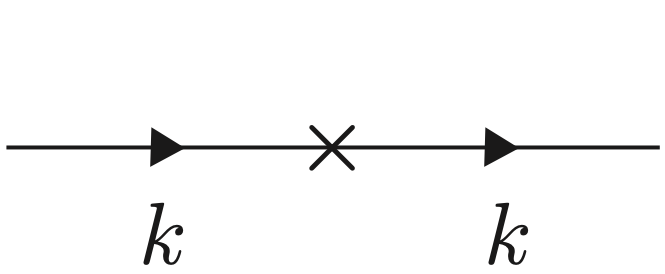
\includegraphics[align=c, width=0.2\linewidth]{pics/KG-ct.png}.
\end{aligned}
\end{equation}



\subsection{Self Energy Correction}
To second order, we consider the one-loop correction to the propagator: 
\begin{equation}\label{eq:rkg-self-energy}
\begin{aligned}
	i\tilde{\Delta}^{(2)}(k) 
	&= 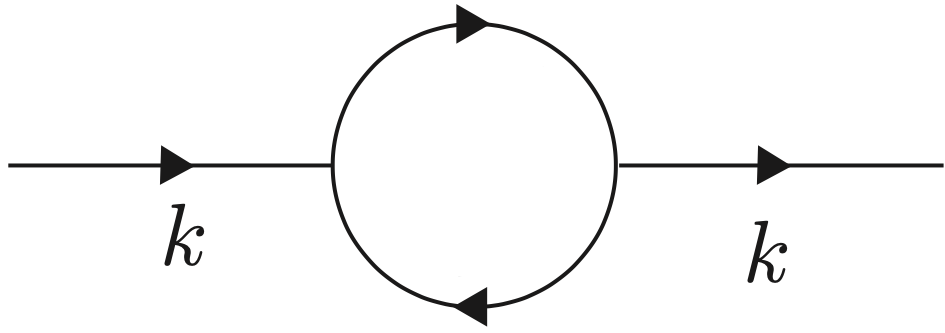
\includegraphics[align=c, width=0.2\linewidth]{pics/KG-1.png} \\
	&= i\tilde\Delta_0(k)\left[i\Sigma^{(2)}(k^2)\right]i\tilde\Delta_0(k),
\end{aligned}
\end{equation}
where the self energy term to the second order $i\Pi^{(2)}(k)$ is defined as:
\begin{equation}
	i\Sigma^{(2)}(k^2) 
	\equiv \frac{g^2}{2} \int \frac{d^dq}{(2\pi)^d} \tilde{\Delta}_0(q)\tilde{\Delta}_0(k-q) + (Ak^2-Bm^2).
\end{equation}

The coefficient $g^2/2$ comes from the symmetry factor in the diagram. We can also check the coefficient explicitly, by considering the expansion to the second order (we denote $\delta/\delta J(x_i)$ as $\delta_i$):
\begin{equation*}
\begin{aligned}
	\delta_{1}\delta_{2}\frac{1}{2!4!}\left[\frac{ig}{3!}\int d^dy \left(\frac{\delta}{\delta J(y)}\right)^3 \right]^2
	\left[-\frac{i}{2}\int d^dy_1 d^dy_2 J(y_1)\Delta(y_1-y_2)J(y_2)\right]^4.
\end{aligned}
\end{equation*}
The expansion gives the coefficient
\begin{equation*}
	\left(\frac{ig}{6}\right)^2\times \frac{1}{2!\times 4! \times 2^4}.
\end{equation*}
Now consider the combinatorial factor, which comes from the exchange of $\phi(x_i)$ in the propagator, the exchange of $\phi(x_i)$ in the vertex, the exchange of propagator in the diagram, and the change of vertices in the diagram:
\begin{equation*}
	(2!)^4\times(3!)^2\times(4\times 3)\times2.
\end{equation*}
Those two factors produce a $-g^2/2$ coefficient.
Note that in the self energy expressio, we put a $i$ factor in front of each propagator, which absorbs the minus sign.


Once we obtain the self energy, the one-loop corrected propagator has the form:
\begin{equation}
\begin{aligned}
	i\tilde{\Delta}(k) 
	&= i\tilde{\Delta}_0(k) + i\tilde{\Delta}_0(k)\left[\sum_{n=1}^{\infty}i\Sigma(k^2)\right]i\tilde{\Delta}_0(k) \\
	&= \frac{i}{\tilde{\Delta}^{-1}_0(k) - \Sigma(k^2)} \\
	&= \frac{i}{k^2-m^2-\Sigma(k^2)}.
\end{aligned}
\end{equation}
Now we are going to evaluate the divergent integral in the self energy expression, using the Feynman parameters:
\begin{equation*}
\begin{aligned}
&\int \frac{d^d q}{(2 \pi)^d} \frac{1}{q^{2}-m^2} \frac{1}{(k-q)^{2}-m^2} \\
=&\int \frac{d^d q}{(2 \pi)^d} \int_{0}^{1} d x \frac{1}{\left[q^{2}-m^2+x\left((q-k)^{2}-q^{2}\right)\right]^{2}} \\
=&\int_{0}^{1} d x \int \frac{d^d q}{(2 \pi)^d} \frac{1}{\left[(q-kx)^{2}-D\right]^{2}},
\end{aligned}
\end{equation*}
where $D=m^2-k^{2} x(1-x)$. Then we can shift $q \rightarrow q+kx$ leaving an integral that only depends on $q^{2}$. In this way,
\begin{equation*}
\Sigma(k^2) = \int_0^1 I(x)dx.
\end{equation*}
To evaluate the self-energy, it suffices to obtain the integral
\begin{equation*}
I(x) = \frac{g^2}{2i}\int \frac{d^d q}{(2 \pi)^d} \frac{1}{\left[q^{2}-D\right]^{2}}.
\end{equation*}

\begin{framedrmk}[Feyman Parameters]
We use Feynman's formula to combine denominators,
\begin{equation}
\frac{1}{A_{1} \ldots A_{n}}=\int d F_{n}\left(x_{1} A_{1}+\ldots+x_{n} A_{n}\right)^{-n},
\end{equation}
where the integration measure over the Feynman parameters $x_{i}$ is
\begin{equation}
\int d F_{n}=(n-1) ! \int_{0}^{1} d x_{1} \ldots d x_{n} \delta\left(x_{1}+\ldots+x_{n}-1\right).
\end{equation}
This measure is normalized so that $\int d F_{n} =1$. 
The simplest case is
\begin{equation}
\frac{1}{A B}=\int_{0}^{1} \frac{dx}{[A+(B-A) x]^{2}}
=\int_{0}^{1} \frac{\delta(x+y-1)}{[x A+y B]^{2}} dx dy.
\end{equation}
Other useful identities are
\begin{equation}
\begin{aligned}
\frac{1}{A B^{n}} &=\int_{0}^{1} dxdy\frac{\delta(x+y-1)n y^{n-1}}{[x A+y B]^{n+1}} , \\
\frac{1}{A B C} &=\int_{0}^{1} dxdydz \frac{2\delta(x+y+z-1)}{[x A+y B+z C]^{3}} .
\end{aligned}
\end{equation}
\end{framedrmk}


By making the Wick rotation $q^0 \rightarrow i q_E^0$, the integral becomes:\footnote{
	The $d$-dimensional solid angle is
	\begin{equation}
		\Omega_d = \frac{2\pi^{d/2}}{\Gamma(\frac{d}{2})},
	\end{equation}
	where $\Gamma(x)$ is the gamma function, satisfing
	\begin{equation}
		\Gamma(1+x) = x\Gamma(x),\ 
		\Gamma(\epsilon) = \frac{1}{\epsilon}-\gamma_E + O(\epsilon).
	\end{equation}
	In particular, $\Gamma(n+1)=n!$.
}
\begin{equation*}
I(x) = \frac{g}{2}\int \frac{d^d q_E}{(2 \pi)^d} \frac{1}{\left(q_E^{2}+D\right)^{2}}
=\frac{g\Omega_d}{2(2\pi)^d} \int dq \frac{q^{d-1}}{\left(q^{2}+D\right)^{2}}.
\end{equation*}


\subsubsection*{Dimensional Regularization}
We set the dimension to $d=6-\epsilon$, and rewrite the Lagrangian as
\begin{equation}
	\mathcal L 
	= Z_{\phi}\frac{1}{2} \partial^\mu\phi\partial_\mu\phi - 
	Z_m \frac{m^2}{2}\phi^2 + Z_g\frac{g\tilde{\mu}^{\epsilon/2}}{3!}\phi^3.
\end{equation}
Note that the coupling constant should be changed to $g\rightarrow g\tilde\mu^{\epsilon/2}$ where $\mu$ is of mass dimension $[1]$ in order to get the correct dimensionality. 
We then expand the expression to zeroth order of $\epsilon$.
A useful identity is:
\begin{equation}
\int d k \frac{k^{a}}{\left(k^{2}+D\right)^{b}}
= D^{\frac{a+1}{2}-b} 
\frac{\Gamma\left(\frac{a+1}{2}\right)\Gamma\left(b-\frac{a+1}{2}\right)}{2\Gamma(b)}.
\end{equation}
Actually, we can compute the integral and series expansion in \texttt{Mathematica} all together:
\FrameTBStyle{mathematica}
\begin{lstlisting}[style=mathematicaFrameTB]
omg=(2*Pi^(d/2))/(Gamma[d/2]);
cof=g^2*\[Mu]^(6-d)/2*omg/(2*Pi)^d;
int=cof*Integrate[q^(d-1)/(q^2+D)^2,{q,0,Infinity}][[1]];
map={g^2->\[Alpha]*(4*Pi)^3,EulerGamma->Subscript[\[Gamma],E]};
ans=Series[int/.{d->6-\[Epsilon]},{\[Epsilon],0,0}];
ans/.map//Simplify
\end{lstlisting}
The result is (where $\alpha\equiv g^2/(4\pi)^3$)
\begin{equation*}
I(x)= \frac{\alpha D}{2} \left[
\ln \left(\frac{De^{\gamma_E}}{4\pi\tilde\mu^2}\right)-\left(\frac{2}{\epsilon}+1\right)
\right]+O(\epsilon).
\end{equation*}
Now insert $D=m^2-k^{2} x(1-x)$. Note that
\begin{equation*}
\int_0^1 dx D = m^2-\frac{k^2}{6}.
\end{equation*}
This simplifies the result to
\begin{equation}
	\Sigma^{(2)}(k^2) = \frac{\alpha}{2}\left(\frac{2}{\epsilon}+1\right)\left(\frac{k^2}{2}-m^2\right)
	+ \frac{\alpha}{2}\int_0^1 dx D(x)\ln\left(\frac{D(x)}{\mu^2}\right),
\end{equation}
where we have replace $\tilde\mu$ with
\begin{equation}
\mu \equiv \sqrt{\frac{4\pi}{e^{\gamma_E}}}\tilde\mu.
\end{equation}



\subsubsection*{Renormalization}
 
The counter terms also contribute to the perturbative correction,
\begin{equation*}
\begin{aligned}
	\Sigma^{(2)}\left(k^{2}\right) 
	=& \frac{\alpha}{2} \int_{0}^{1} dx D \ln\left(\frac{D}{m^{2}}\right) 
	+\left\{\frac{\alpha}{6}\left[\frac{1}{\varepsilon}+\ln\left(\frac{\mu}{m}\right)+\frac{1}{2}\right]+A\right\} k^{2} \\
	&-\left\{\alpha\left[\frac{1}{\varepsilon}+\ln\left(\frac{\mu}{m}\right)+\frac{1}{2}\right]+B\right\} m^{2}+O\left(\alpha^{2}\right) .
\end{aligned}
\end{equation*}
Consider the on-shell condition for the subtraction:
\begin{equation}
	\Sigma(m^2) = \Sigma'(m^2)=0.
\end{equation}
Set $D_0 \equiv D(x)|_{k^2=m^2}=m^2(1-x+x^2)$, the self energy has the form:
\begin{equation}
	\Sigma^{(2)}(k^2)=\frac{\alpha}{2} \int_0^1dx D(x)\ln\left(\frac{D(x)}{D_0(x)}\right) + C_k k^2+C_m m^2.
\end{equation}
The condition $\Pi(m^2) =0$ requires
\begin{equation*}
	\Sigma^{(2)}(k^2)=\frac{\alpha}{2} \int_0^1dx D(x)\ln\left(\frac{D(x)}{D_0(x)}\right) + C_k (k^2-m^2).
\end{equation*}
The condition $\Pi'(m^2)=0$ requires
\begin{equation*}
\begin{aligned}
	\left.\frac{d\Sigma^{(2)}(k^2)}{dk^2}\right|_{k^2=m^2}
	&=\frac{\alpha}{2} \int_0^1dx \left.\left[
	\frac{D(x)}{dk^2}\ln\left(\frac{D(x)}{D_0(x)}\right)+D_0(x)
	\right]\right|_{q^2=m^2} + C_k  \\
	&= \frac{\alpha}{2}\int_0^1dx (x^2-x) + C_k \\
	&= C_k-\frac{\alpha}{12} = 0.
\end{aligned}
\end{equation*}
In this way, we obtained the renormalized self-energy:
\begin{equation}
	\Sigma^{(2)}(k^2)=\frac{\alpha}{2} \int_0^1dx D(x)\ln\left(\frac{D(x)}{D_0(x)}\right) + \frac{\alpha}{12}(k^2-m^2).
\end{equation}

On the other hand, we chan choose the $\overline{\mathrm{MS}}$ subtraction scheme, i.e.,
\begin{equation}
	A = -\frac{\alpha}{6\epsilon},\ 
	B = -\frac{\alpha}{\epsilon}.
\end{equation}
The self energy under $\overline{\mathrm{MS}}$ scheme will depend on the the mass scale $\mu$ we choose:
\begin{equation}
	\Sigma^{(2)}\left(k^{2}\right) 
	= \frac{\alpha}{2} \int_{0}^{1} dx D \ln\left(\frac{D}{m^{2}}\right) 
	+\alpha\left[\ln\left(\frac{\mu}{m}\right)+\frac{1}{2}\right]\left(\frac{k^2}{6}-m^2\right).
\end{equation}


\subsection{Vertex Correction}
Now consider the simplest one-loop correction to the vertex function (together with the counter term):
\begin{equation}
\begin{aligned}
	i V_3^{(3)}(k_{1}, k_{2}, k_{3})
	&= 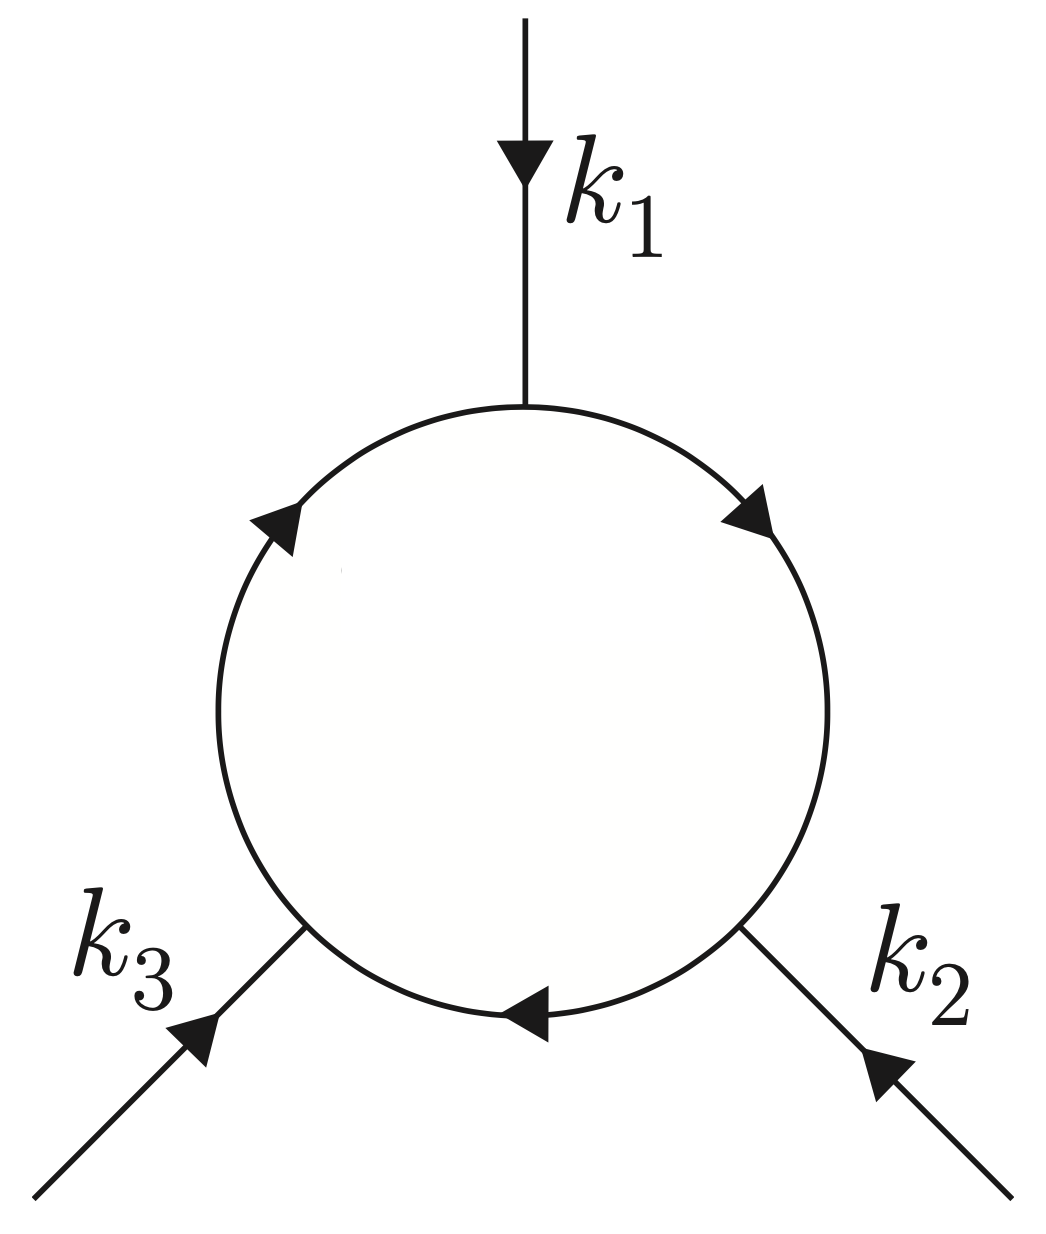
\includegraphics[align=c, width=0.4\linewidth]{pics/KG-2.png} \\
	&= (ig)^3i^3 \int \frac{d^{a} q}{(2 \pi)^{d}} \tilde{\Delta}(q-k_{1}) \tilde{\Delta}(q+k_{2}) \tilde{\Delta}(q) + i Cg,
\end{aligned}
\end{equation}
Using the Feynman parameter, the integrant is
\begin{equation*}
\tilde{\Delta}(q-k_{1}) \tilde{\Delta}(q+k_{2}) \tilde{\Delta}(q) 
= \int d F_3\frac{1}{(q^2-D)^3}
\end{equation*}
where we have shift the value of $q$, and $D$ can be evaluate by the following code:
\begin{lstlisting}[style=mathematicaFrameTB]
A1=(l-k1)^2-m^2;
A2=(l+k2)^2-m^2;
A3=(l)^2-m^2;
{c,b,a}=CoefficientList[x1*A1+x2*A2+(1-x1-x2)*A3,{l}];
-c+b^2/(4*a)//Expand
\end{lstlisting}
The result is
\begin{equation*}
D = m^2-k_1^2 x_1 (1- x_1)-k_2^2 x_2 (1- x_2)-2 k_1 k_2 x_1 x_2.
\end{equation*}
The same procedure gives:
\begin{equation}
	V_3^{(3)}/g = \int dF_3 I(x_1,x_2,x_3) + C,
\end{equation}
where
\begin{equation*}
I(x_1,x_2,x_3) = \frac{g^2 \Omega_d}{(2\pi)^d} \int dq \frac{q^{d-1}}{(q^2+D)^3}.
\end{equation*}
The same regularization procedure in \texttt{Mathematica}:
\begin{lstlisting}[style=mathematicaFrameTB]
omg=(2*Pi^(d/2))/(Gamma[d/2]);
cof=g^2*\[Mu]^(6-d)*omg/(2*Pi)^d;
int=cof*Integrate[q^(d-1)/(q^2+D)^3,{q,0,Infinity}][[1]];
map={g^2->\[Alpha]*(4*Pi)^3,EulerGamma->Subscript[\[Gamma],E]};
ans=Series[int/.{d->6-\[Epsilon]},{\[Epsilon], 0, 0}];
ans/.map//Simplify
\end{lstlisting}
The result is
\begin{equation}
\begin{aligned}
	V_3^{(3)}/g 
	&= \frac{\alpha}{\epsilon}
	+ \frac{\alpha}{2}\int dF_3 \ln\left(\frac{4\pi\tilde{\mu}^2e^{-\gamma_E}}{D}\right) 
	+ C + O(\epsilon) \\
	&= \frac{\alpha}{\epsilon}
	+ \alpha\ln\left(\frac{\mu}{m}\right)
	- \frac{\alpha}{2}\int dF_3 \ln\left(\frac{D}{m}\right)
	+C.
\end{aligned}
\end{equation}
The on-shell subtraction requires 
\begin{equation}
V_3(0,0,0) = g,
\end{equation}
which gives
\begin{equation}
	C = -\frac{\alpha}{\epsilon}-\alpha \ln\left(\frac{\mu}{m}\right).
\end{equation}
So the vertex function to the third order is
\begin{equation}
	V_3(k_1,k_2,k_3) = g\left\{1-\frac{\alpha}{2} \int dF_3 \ln\left[\frac{D(x_1,x_2,x_3)}{m}\right] \right\}.
\end{equation}
The $\overline{\mathrm{MS}}$ scheme, on the other hand, sets
\begin{equation}
	C = -\frac{\alpha}{\epsilon}.
\end{equation}



\subsection{Renormalization Group}
We fist summarize the normalization factor obtained on the one-loop level (with $\overline{\mathrm{MS}}$ subtraction scheme):
\begin{equation}
\begin{aligned}
	Z_{\phi} &= 1-\frac{\alpha}{6\epsilon} + O(\alpha^2), \\
	Z_{m} &= 1-\frac{\alpha}{\epsilon}+ O(\alpha^2), \\
	Z_{g} &= 1-\frac{\alpha}{\epsilon}+ O(\alpha^2).
\end{aligned}
\end{equation}
For the renormalized Lagrangian in ($6-\epsilon$)-dimension
\begin{equation}
	\mathcal L 
	= Z_{\phi}\frac{1}{2} \partial^\mu\phi\partial_\mu\phi - 
	Z_m \frac{m^2}{2}\phi^2 + Z_g\frac{g\tilde{\mu}^{\epsilon/2}}{3!}\phi^3,
\end{equation}
the factors relate the original field and bare coefficients
\begin{equation}
	\phi_0 = Z_\phi^{1/2}\phi,\ 
	m_0 = Z_m^{1/2} Z_\phi^{-1/2}m,\ 
	g_0 = Z_g Z_{\phi}^{-3/2} \tilde{\mu}^{\epsilon/2}g.
\end{equation}
The renormalization group requires that the bare parameter is independent of the mass scale $\mu$ we choose, that is:
\begin{equation}
	\frac{d\phi_0}{d \ln \mu} 
	= \frac{dm_0}{d \ln \mu}
	= \frac{dg_0}{d \ln \mu}
	= 0.
\end{equation}


\subsubsection*{Beta Function}
Star with $g_0$, it is more convenient to use 
\begin{equation}
\alpha_0 
\equiv \frac{g_0^2}{4\pi} 
= Z_g^2 Z_{\phi}^{-3}\tilde{\mu}^{\epsilon}\alpha.
\end{equation}
Take logarithm on both side:
\begin{equation}
\ln \alpha_0 = \ln(Z_g^2 Z_{\phi}^{-3}) 
+ \ln \alpha + \epsilon\ln{\tilde\mu}.
\end{equation}
The RG equation is
\begin{equation}
\frac{d \ln \alpha_0}{d \ln \mu} = 
\frac{d \ln(Z_g^2 Z_{\phi}^{-3}) }{d \alpha}\frac{d \alpha}{d\ln \mu} +
\frac{1}{\alpha}\frac{d \alpha}{d \ln \mu} + \epsilon
=0.
\end{equation}
To the first order of $\alpha$:
\begin{equation}
\begin{aligned}
	\frac{d \ln(Z_g^2 Z_{\phi}^{-3}) }{d \alpha}
	=\frac{d}{d\alpha}\left(-\frac{2\alpha}{\epsilon}+\frac{\alpha}{2\epsilon}\right) 
	= -\frac{3}{2\epsilon},
\end{aligned}
\end{equation}
which leads to
\begin{equation}
	\frac{d\alpha}{d\ln \mu}\left(1-\frac{3\alpha}{2\epsilon}+O(\alpha^2)\right)+\epsilon\alpha = 0.
\end{equation}
The beta function is defined as
\begin{equation}
	\beta(\alpha) = \frac{d\alpha}{d\ln \mu} = \beta_1 \alpha + \beta_2 \alpha^2 + O(\alpha^3).
\end{equation}
Insert such definition into the original expression, and keep track of the order of $\alpha$, we get
\begin{equation}
	(\beta_1+\epsilon)\alpha + \left(\beta_2-\frac{3\beta_1}{2\epsilon}\right)\alpha^2 + O(\alpha^3) = 0.
\end{equation}
The beta function is
\begin{equation}
	\beta(\alpha) = -\epsilon \alpha -\frac{3}{2}\alpha^2 + O(\alpha^3).
\end{equation}



\subsubsection*{Anomalous Dimension}
Consider the RG equation with bare mass:
\begin{equation}
\begin{aligned}
\frac{d\ln m_0}{d\ln \mu} 
&= \frac{1}{2}\frac{d(\ln Z_m - \ln Z_\phi)}{d\alpha}\frac{d\alpha}{d\ln\mu}
	+\frac{1}{m}\frac{d m}{d\ln \mu} \\
&= \frac{5\alpha}{12}+\frac{1}{m}\frac{d m}{d\ln \mu} + O(\alpha^2) = 0.
\end{aligned}
\end{equation}
We get the anomalous dimension of the mass:
\begin{equation}
\gamma_m(\alpha) \equiv \frac{1}{m}\frac{d m}{d\ln \mu} 
= -\frac{5\alpha}{12}+O(\alpha^2).
\end{equation}
Also, for the bare field
\begin{equation}
\frac{d\ln\phi_0}{d\ln\mu} = \frac{1}{2} \frac{d\ln Z_{\phi}}{d\ln\mu} 
+ \frac{d\ln\phi}{d\ln\mu} = 0.
\end{equation}
We can define the anomalous dimension of the field as
\begin{equation}
\gamma_{\phi} \equiv \frac{1}{2}\frac{d \ln Z_\phi}{d\ln\mu}
= \frac{1}{2}\frac{d \ln Z_\phi}{d\alpha}\frac{d\alpha}{d\ln\mu}
= \frac{\alpha}{12} +O(\alpha^2).
\end{equation}



\subsubsection*{Callan-Symanzik Equation}
Consider the bare propagator:
\begin{equation}
\tilde{\Delta}_0(k) = Z_\phi \tilde{\Delta}(k)
\end{equation}
The RG condition for the bare propagator gives:
\begin{equation*}
\frac{d\ln\tilde{\Delta}_0(k)}{d \ln\mu}
=\frac{d\ln Z_\phi}{d\ln\mu}+\frac{1}{\tilde{\Delta}(k)}\left(
	\frac{\partial}{\partial\ln\mu} +
	\frac{d\alpha}{d\ln\mu}\frac{\partial}{\partial\alpha} +
	\frac{dm}{d\ln\mu}\frac{\partial}{\partial m}
\right)\tilde{\Delta}(k)=0.
\end{equation*}
The Callan-Symanzik equation is
\begin{equation}
	\left(
	2\gamma_\phi+
	\frac{\partial}{\partial\ln\mu} +
	\beta(\alpha)\frac{\partial}{\partial\alpha} +
	\gamma_m(\alpha)m\frac{\partial}{\partial m}
\right)\tilde{\Delta}(k)=0.
\end{equation}

\section{Real $\phi^4$ Theory}
In this section, we consider the real Klein-Gordon field with $\phi^4$ interaction.
The field $\phi$ has mass dimension $[\frac{d-2}{2}]=[1]$, so the critical dimension is $d=4$, where the coupling constant $g$ is dimensionless.
For dimensional regulation purpose, we write the renormalized Lagrangian on $(4-\epsilon)$-dimensional space-time as
\begin{equation}
	\mathcal{L}
	= Z_{\phi}\frac{1}{2} \partial^\mu\phi\partial_\mu\phi - 
	Z_m \frac{m^2}{2}\phi^2 - Z_g\frac{g \tilde{\mu}^\epsilon}{4!}\phi^4,
\end{equation}
where we have introduced a mass scale $\tilde \mu$.
As the $\phi^3$ theory, we can rewrite the Lagrangian as:
\begin{equation}
	\mathcal L = \mathcal L_0 + \mathcal L_{\mathrm{int}} + \mathcal L_{\mathrm{ct}}.
\end{equation}
In the following we investigate the loop correction to the mass and the coupling constant.


\subsection{One-loop Correction}
\subsubsection*{Self-energy}
Following the same procedure, the one-loop self-energy correction is (with counter terms):
\begin{equation}
\begin{aligned}
	i\Sigma(k^2) 
	&= 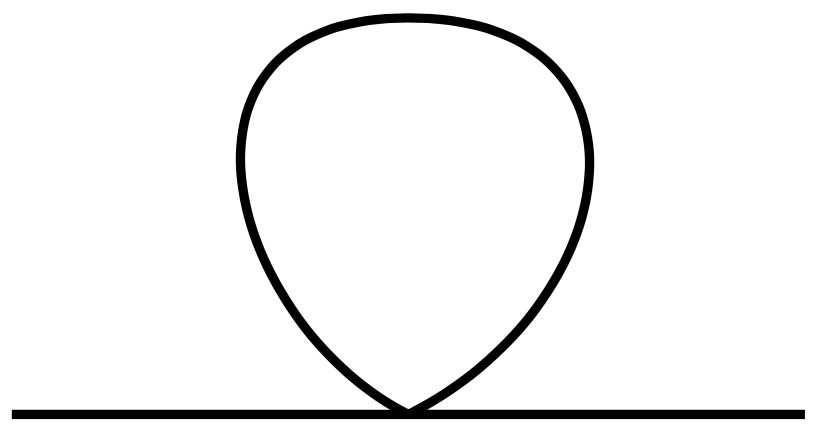
\includegraphics[align=c, width=0.4\linewidth]{pics/KG-3.png} \\
	&= -\frac{g\tilde{\mu}^\epsilon}{2}\int \frac{d^d q}{(2\pi)^d} \frac{1}{q^2-m^2} + i(Ak^2-Bm^2).
\end{aligned}
\end{equation}
After the Wick rotation, 
\begin{equation}
	\Sigma(k^2) = -\frac{g\tilde{\mu}^\epsilon}{2}\frac{\Omega_d}{(2\pi)^d} \int \frac{q^{d-1} dq}{q^2+m^2} + (Ak^2-Bm^2).
\end{equation}
The dimensional regulation is carried out using the following code:
\begin{lstlisting}[style=mathematicaFrameTB]
omg=(2*Pi^(d/2))/(Gamma[d/2]);
cof=g*\[Mu]^(4-d)/2*omg/(2*Pi)^d;
int=cof*Integrate[q^(d-1)/(q^2+m^2),{q,0,Infinity}][[1]];
map={EulerGamma->Subscript[\[Gamma],E]};
ans=Series[int/.{d->4-\[Epsilon]},{\[Epsilon],0,0}];
ans/.map//Simplify
\end{lstlisting}
The result is
\begin{equation}
	\Sigma(k^2) = \frac{g m^2}{32\pi^2} \left[\frac{2}{\epsilon}+1+\log \left(\frac{4 \pi \tilde{\mu}^2 e^{-\gamma_E}}{m^2}\right)\right]+(Ak^2-Bm^2)+O(\epsilon).
\end{equation}
Using the $\overline{\mathrm{MS}}$ renormalization scheme, we set
\begin{equation}
	A = 0,\ B = \frac{g}{16\pi^2\epsilon}.
\end{equation}
The result is
\begin{equation}
	\Sigma(k^2) = \frac{g m^2}{16\pi^2} \log \left(\frac{\mu}{m}\right)
	+\frac{g m^2}{32\pi^2}+O(\epsilon).
\end{equation}

\subsubsection*{Vertex Correction}
Now consider the vertex correction.
The vertex correction to the lowest order (with the counter term) is
\begin{equation}
\begin{aligned}
	iV_4^{(2)}(k_1,k_2,k_3,k_4) 
	&= 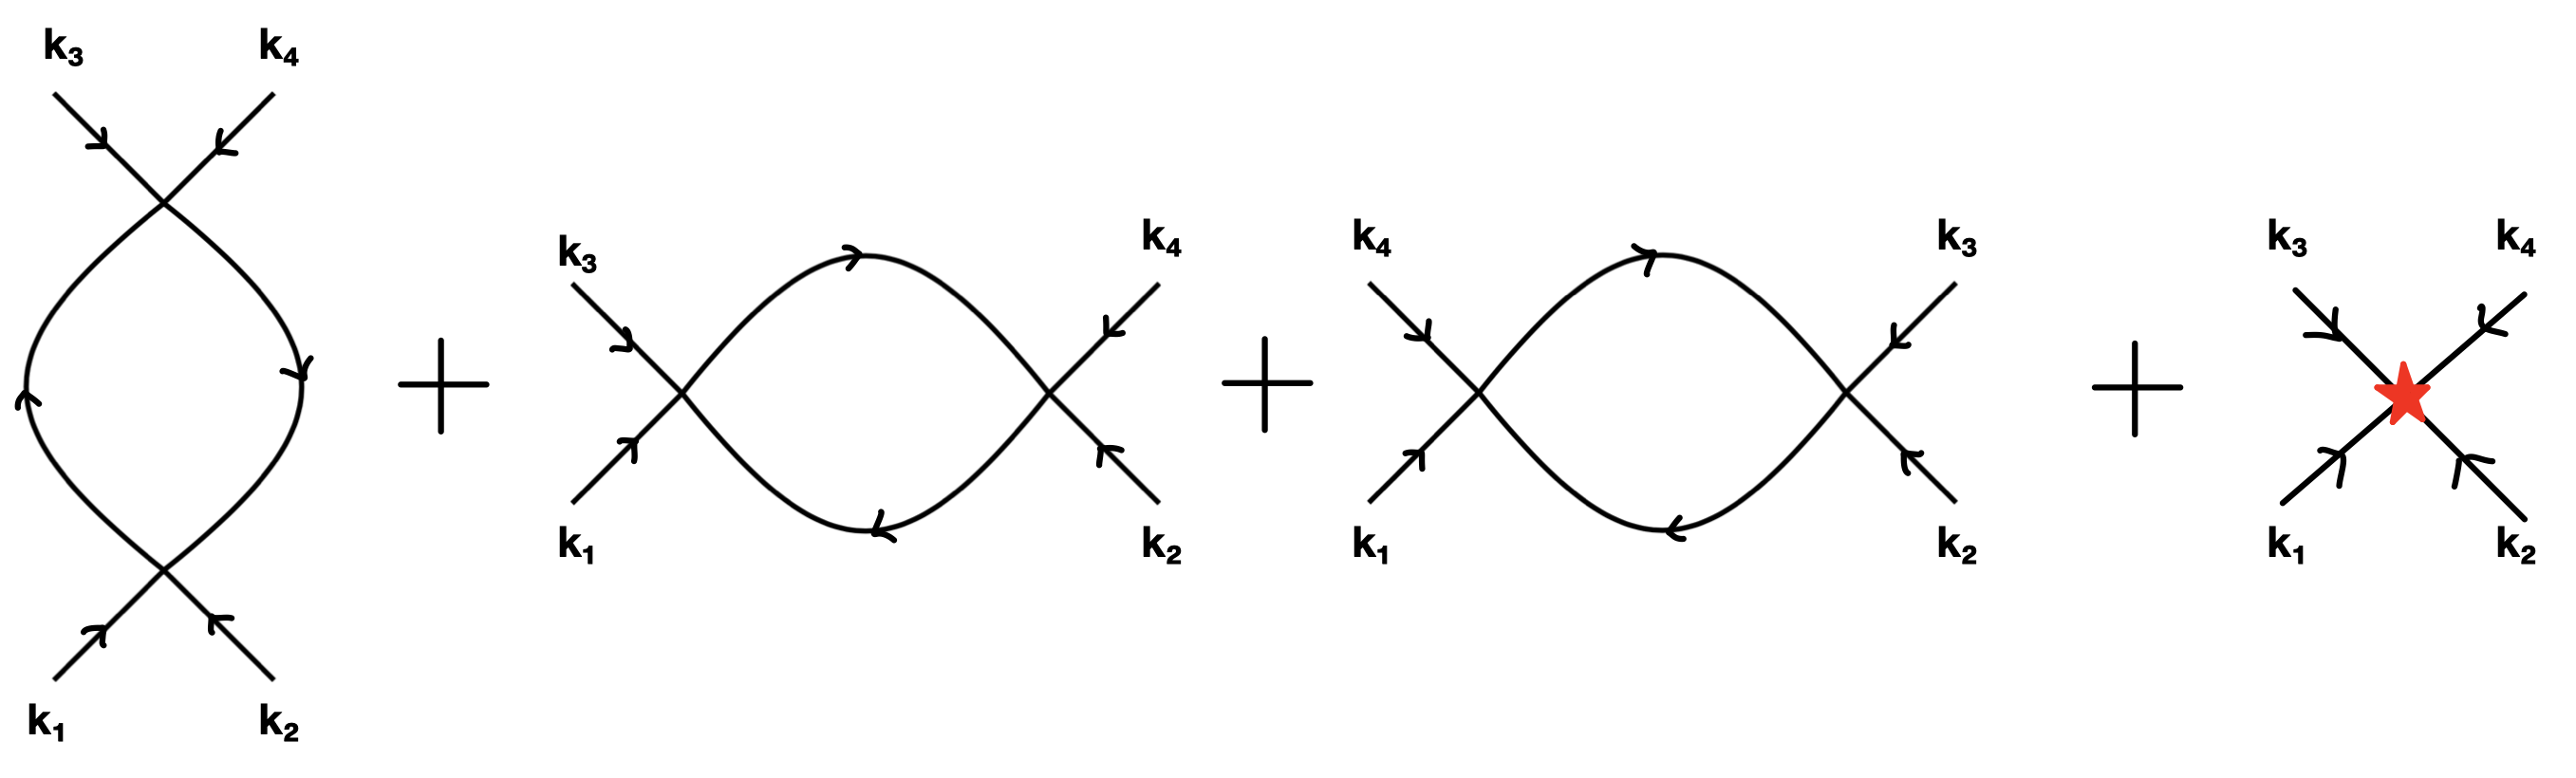
\includegraphics[align=c, width=0.6\linewidth]{pics/KG-4.png}\\
	&= \frac{g^2}{2} \left[iF(s)+iF(t)+iF(u)\right] -iCg,
\end{aligned}
\end{equation}
where
\begin{equation}
	s = (k_1+k_2)^2,\ 
	t = (k_1+k_3)^2,\ 
	u = (k_1+k_4)^2,
\end{equation}
and
\begin{eqnarray}
	iF(k^2) 
	&=& \tilde{\mu}^{\epsilon}\int \frac{d^d q}{(2\pi)^d} \tilde{\Delta}_0(q)\tilde{\Delta}_0(q+k) \\
	&=& \frac{i\tilde{\mu}^{\epsilon}\Omega_d}{(2\pi)^d} \int_0^1 dx \int \frac{q^{d-1}dq}{\left[q^2+m^2+x(1-x)k^2\right]^2}.
\end{eqnarray}
Then we carry out the calculation (set $D(k^2,x)=m^2+x(1-x)k^2$)
\begin{lstlisting}[style=mathematicaFrameTB]
omg=(2*Pi^(d/2))/(Gamma[d/2]);
cof=g^2*\[Mu]^(4-d)/2*omg/(2*Pi)^d;
int=cof*Integrate[q^(d-1)/(q^2+D)^2,{q,0,Infinity}][[1]];
map={EulerGamma->Subscript[\[Gamma],E]};
ans=Series[int/.{d->4-\[Epsilon]},{\[Epsilon],0,0}];
ans/.map//Simplify
\end{lstlisting}
The result is:
\begin{equation}
\begin{aligned}
	F(s) &= \frac{1}{8\pi^2\epsilon} + \frac{1}{16\pi^2}\int_0^1 dx \ln \left(\frac{4\pi \tilde{\mu}^2 e^{-\gamma_E}}{D}\right) \\
	&= \frac{1}{8\pi^2\epsilon} +\frac{1}{8\pi^2}\ln \left(\frac{\mu}{m}\right) - \frac{1}{16\pi^2}\int_0^1 dx \ln\left(\frac{D(s,x)}{m^2}\right).
\end{aligned}
\end{equation}
The $\overline{\mathrm{MS}}$ scheme absorbs the $\frac{1}{8\pi^2\epsilon}$ term, i.e.,
\begin{equation}
	C = \frac{3g}{16\pi^2}.
\end{equation}
The result is:
\begin{equation}
	V_4(k_1,k_2,k_3,k_4) = -g+\frac{g^2}{32\pi^2}\int_0^1 dx \ln\left(\frac{\mu^6}{D(s,x)D(t,x)D(u,x)}\right).
\end{equation}
To summarize, the normalization is:
\begin{eqnarray}
	Z_{\phi} &=& 1, \\
	Z_{m} &=& 1+\frac{g}{16\pi^2 \epsilon}, \\
	Z_{g} &=& 1+\frac{3g}{16\pi^2 \epsilon}.
\end{eqnarray}


\subsection{Renormalization Group}
Now consider the RG equation for the one-loop correction. 
The bare parameters are:
\begin{equation}
	g_0 = Z_g g\tilde{\mu}^{\epsilon},\ 
	m_0 = Z_m^{1/2} m,
\end{equation}
The RG conditions are:
\begin{eqnarray}
	\frac{d g_0}{d\ln \mu}
	&=& \left(\frac{3}{16\pi^2 \epsilon} + \frac{1}{g}\right)\frac{dg}{d\ln \mu} + \epsilon = 0, \\
	\frac{d m_0}{d\ln \mu}
	&=& \frac{1}{32\pi^2 \epsilon}\frac{dg}{d\ln \mu} + \frac{1}{m}\frac{dm}{d \ln \mu} = 0.
\end{eqnarray}
Consider the series expansion of beta function:
\begin{equation}
	\beta(g) = \frac{dg}{d\ln \mu} = \beta_1 g + \beta_2 g^2 +O(g^3).
\end{equation}
The beta function is
\begin{equation}
	\beta(g) = -\epsilon g + \frac{3g^2}{16\pi^2} + O(g^3).
\end{equation}
The anomalous dimension of mass is
\begin{equation}
	\gamma_m = \frac{1}{m}\frac{dm}{d \ln \mu} = \frac{g}{32\pi^2}+O(g^2)
\end{equation}




\chapter{Quantum Electrodynamics}

The Lagrangian for quantum electrodynamics is
\begin{equation}
\begin{aligned}
	\mathcal{L}_{\mathrm{QED}}
	&= \bar\psi \left(i\gamma^\mu \partial_\mu - m\right)\psi - \frac{1}{4}F_{\mu\nu}F^{\mu\nu} -eA_\mu \bar\psi\gamma^\mu  \psi \\
	&= \mathcal{L}_{\mathrm{Dirac}}+\mathcal{L}_{\mathrm{Maxwell}}+\mathcal{L}_{\mathrm{int}},
\end{aligned}
\end{equation}
where
\begin{equation}
	F_{\mu\nu} = \partial_\mu A_\nu - \partial_\nu A_\nu = (dA)_{\mu\nu}.
\end{equation}
The Lagrangian is invariant under the gauge transformation:
\begin{equation}
\begin{aligned}
	\psi(x) &\rightarrow e^{-ie\alpha(x)}\psi(x), \\
	A^\mu(x) &\rightarrow A^\mu(x) + \partial^\mu \alpha(x).
\end{aligned}
\end{equation}
It is convenient to rewrite Lagrangian as
\begin{equation}
	\mathcal{L}_{\mathrm{QED}}
	= \bar\psi \left(i\cancel{D} - m\right)\psi - \frac{1}{4}F_{\mu\nu}F^{\mu\nu},
\end{equation}
where we have define the covariant derivative as:
\begin{equation}
	\cancel{D} = \gamma^\mu D_\mu 
	= \gamma^\mu [\partial_\mu + i e A_\mu(x)]
	= \cancel{\partial} + ie \cancel{A}.
\end{equation}


\section{Free Field Theory}

\subsection{Dirac Field}
The free Dirac field is
\begin{equation}
	\mathcal{L}_{\mathrm{Dirac}}
	= \bar\psi \left(i\gamma^\mu \partial_\mu - m\right)\psi
\end{equation}
Consider the partition function with source
\begin{equation}
\begin{aligned}
	Z_{\mathrm{Dirac}}[J]
	&= \int D[\bar\psi,\psi] \exp\left[i\int d^dx \left(\mathcal{L}_{\mathrm{Dirac}}+\bar{\eta}\psi + \bar\psi\eta \right) \right] \\
	&= Z_{\mathrm{Dirac}}[0] \exp\left[-i\int d^dx_1 d^d x_2 \bar{\eta}(x_1)\cdot D_F(x_1-x_2)\cdot \eta(x_2) \right].
\end{aligned}
\end{equation}
where
\begin{equation}
	D_F(x_1-x_2) = \int \frac{d^d k}{(2\pi)^d} \frac{e^{-i k \cdot (x_1-x_2)}}{\cancel{k}-m}
	= \int \frac{d^d k}{(2\pi)^d} e^{-i k \cdot (x_1-x_2)} \frac{\cancel{k}+m}{k^2-m^2}.
\end{equation}
Note that the propagator is\footnote{The sign in the variational derivative comes from the anti-commutation relation of the fermionic fields.}
\begin{equation}
\begin{aligned}
	\langle 0| T \psi(x_1) \bar\psi(x_2) |0\rangle
	&= \frac{1}{Z_{\mathrm{Dirac}}[0]}\frac{\delta}{i\delta \bar{\eta}(x_1))}\frac{i\delta}{\delta(\eta(x_2))} Z_{\mathrm{Dirac}}[J] \\
	&= i D_F(x_1-x_2).
\end{aligned}
\end{equation}

\subsection{Electromagnetic Field}
The Lagrangian for the classical electromagnetic field is
\begin{equation}
	\mathcal{L} = -\frac{1}{4}F_{\mu\nu}F^{\mu\nu}+A_\mu J^\mu.
\end{equation}
Consider the partition function
\begin{equation}
	\frac{Z_{\mathrm{maxwell}}[J]}{Z_{\mathrm{maxwell}}[0]}
	= \exp\left[-\frac{i}{2}\int dx_1 dx_2 J_\mu(x_1) \Pi^{\mu\nu}(x_1-x_2) J_\nu(x_2) \right].
\end{equation}

The propagator is
\begin{equation}
	\Pi^{\mu\nu}(x_1-x_2) = \int \frac{d^d k}{(2\pi)^d} e^{-ik\cdot(x_1-x_2)}\frac{-g^{\mu\nu}+(1-\xi)k^\mu k^\nu}{k^2}.
\end{equation}


\subsection{Perturbation Theory}
As with the scalar field, 
\begin{equation}
	Z[\bar\eta,\eta,J] = \exp\left\{i\int d^dx \mathcal{L}_{\mathrm{int}}\left[\frac{\delta}{i\delta J},\frac{\delta}{i\delta \eta},\frac{i\delta}{\delta \bar\eta}\right]\right\} Z_0[\bar\eta,\eta,J].
\end{equation}
We use the dimensional regularization by default. 
Note that $\psi$ has the mass dimension $[\frac{d-1}{2}]$, $A^\mu$ had the mass dimension $[\frac{d}{2}-1]$, and $e$ has the mass dimension $[2-\frac{d}{2}]$.
When $d=4-\epsilon$, we replace $e$ with $e \tilde{\mu}^{\epsilon/2}$, so that to make the coupling constant $e$ dimensionless.

The renormalized Lagrangian is
\begin{equation}
\begin{aligned}
	\mathcal L 
		&= Z_{\psi} \bar\psi_R(i\gamma^\mu \partial_\mu)\psi_R 
		-Z_m m \bar\psi_R\psi_R 
		+ \frac{1}{4} Z_{A} F_{R,\mu\nu}F_R^{\mu\nu} - Z_e e_R A_R^\mu \bar\psi_R\gamma^\mu \psi_R \\
		&= \mathcal{L}_0 + \mathcal{L}_{\mathrm{int}} + \mathcal{L}_{\mathrm{ct}}.
\end{aligned}
\end{equation}
The we define the coefficients
\begin{equation}
	\delta_{\psi} = Z_\phi - 1,\ 
	\delta_{m} = Z_m - 1,\ 
	\delta_Z = Z_A - 1, \ 
	\delta_e = Z_e - 1.
\end{equation}
The counter term also contribute to the perturbative expansion like the interactions.


\begin{framedexpl}[One-loop Correction to Electron Propagator]
Consider the diagram
\begin{equation*}
	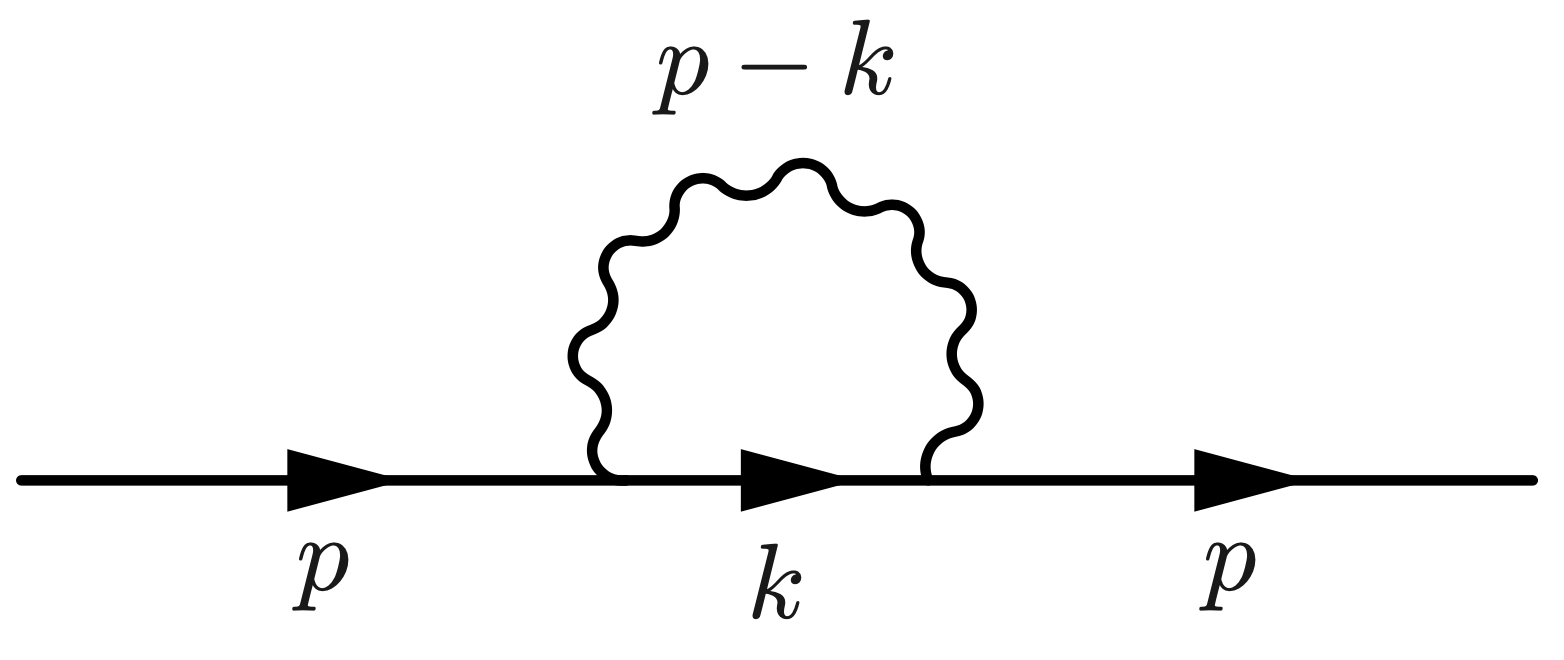
\includegraphics[width=0.3\linewidth]{pics/QED-1.png}
\end{equation*}
This contains 3 electron propagator, 1 photon propagator, and 2 vertices.
The coefficient is (omit all the integration and summation for simplicity):
\begin{equation*}
	iD_F^{(2)}(p) \sim \frac{\delta^2}{\delta\bar\eta \delta\eta}\frac{1}{2!}
	\left(\frac{-ie\gamma^\mu_{\alpha\beta}\delta^3}{i\delta J^\mu \delta\eta_{\alpha} \delta\bar\eta_{\beta}}\right)^2 
	\frac{1}{3!}\left(-i \bar\eta_{\alpha} D_F^{\alpha\beta} \eta_{\beta} \right)^3 
	\left(-\frac{i}{2} J^\mu\Pi_{\mu\nu}J^{\nu} \right).
\end{equation*}
First consider the scalar coefficient. 
Since there is no additional symmetry, the abstract value is $e^2$.
There is an additional sign factor by the proper order of the fermion operators:
\begin{equation*}
	\frac{\delta^2}{\delta\bar\eta_f \delta\eta_i} \frac{\delta^2}{\delta\eta_1 \delta\bar\eta_1} \frac{\delta^2}{\delta\eta_2 \delta\bar\eta_2}
	= - \frac{\delta}{\delta \eta_i}\frac{\delta^2}{\delta\bar\eta_1 \delta\eta_1}\frac{\delta^2}{\delta\bar\eta_2 \delta\eta_2}\frac{\delta}{\delta \bar\eta_f}.
\end{equation*}

Then consider the tensor contraction, 
\begin{equation*}
	\Pi_{\mu\nu} D_F^{\alpha\lambda}\gamma^\mu_{\lambda\rho} D_F^{\rho\tau} \gamma^\nu_{\tau\sigma} D_F^{\sigma\beta}.
\end{equation*}

The total amplitude is
\begin{equation*}
\begin{aligned}
	iD_F^{(2)}(p)
	&= -e^2\int\frac{d^4 k}{(2\pi)^4} \Pi_{\mu\nu}(p-k) \left[D_F(p) \gamma^\mu D_F(k) \gamma^\nu D_F(p)\right]_{\alpha\beta} \\
	&= iD_F(p) i\Sigma(p^2) iD_F(p),
\end{aligned}
\end{equation*}
where $i\Sigma(p^2)$ is the self energy:
\begin{equation}
	i\Sigma(p^2)
	= e^2\int\frac{d^4 k}{(2\pi)^4} \Pi_{\mu\nu}(p-k) \gamma^\mu D_F(k) \gamma^\nu ,
	\label{eq:QED-ele-loop-prop}
\end{equation}
\end{framedexpl}


\begin{framedexpl}[One-loop Correction to Photon Propagator]
Consider the diagram
\begin{equation*}
	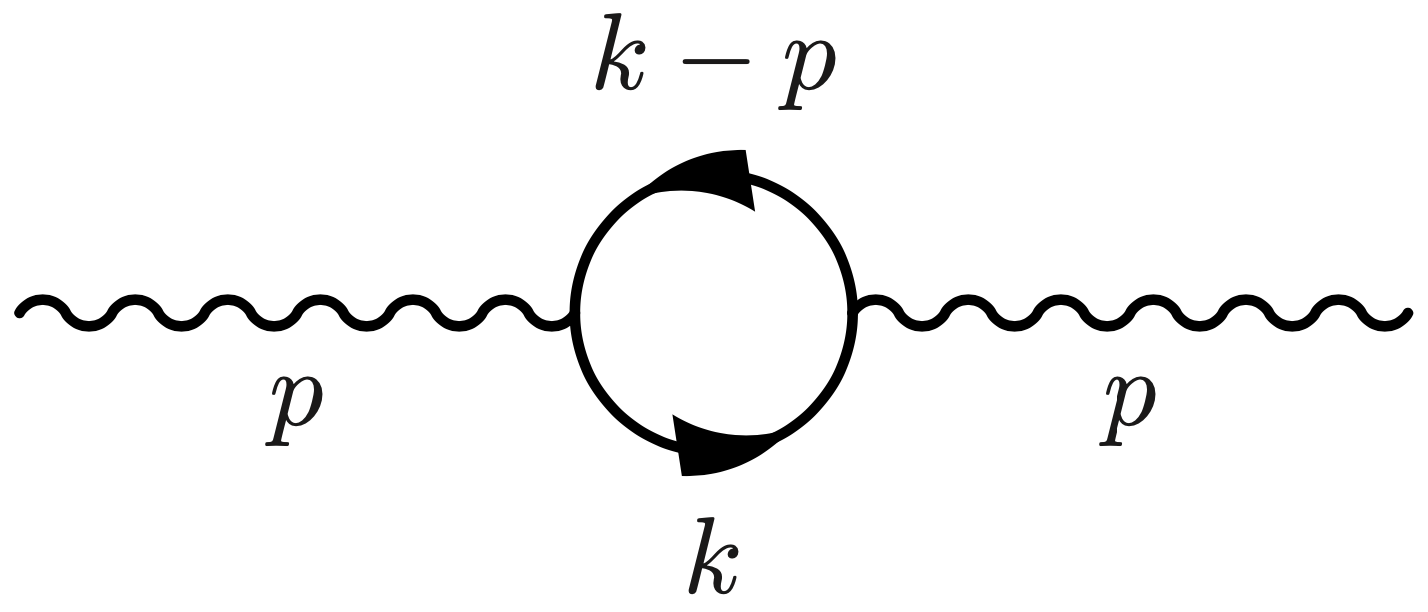
\includegraphics[width=0.3\linewidth]{pics/QED-2.png}
\end{equation*}
There is 2 electron propagator, 2 photon propagator, and 2 vertices.
Consider the perturbative expansion:
\begin{equation*}
	i\Pi^{(2)}(p) \sim \frac{\delta^2}{i\delta J i\delta J}\frac{1}{2!}
	\left(\frac{-e\gamma^\mu_{\alpha\beta}\delta^3}{\delta J^\mu \delta\eta_{\alpha} \delta\bar\eta_{\beta}}\right)^2 
	\frac{1}{2!}\left(-i \bar\eta_{\alpha} D_F^{\alpha\beta} \eta_{\beta} \right)^2 
	\frac{1}{2!}\left(\frac{i}{2} J^\mu \Pi_{\mu\nu} J^{\nu} \right)^2.
\end{equation*}
The diagram has no symmetry factor, but with a $-1$ sign, which is canceled out by the operator reordering:
\begin{equation}
	\bar\eta_\beta D_F^{\beta\tau} \eta_\tau \bar\eta_\sigma D_F^{\sigma\alpha} \eta_\alpha
	= -\eta_\alpha\bar\eta_\beta D_F^{\beta\tau} \eta_\tau \bar\eta_\sigma D_F^{\sigma\alpha}.
\end{equation}
The overall value is $e^2$.
 
Then consider the tensor contraction, 
\begin{equation*}
\begin{aligned}
	-i\Pi_{(2)}^{\mu\nu} 
	&\sim e^2 \Pi_{\mu\rho} \gamma^\rho_{\alpha\beta} D_F^{\beta\tau} \gamma^\eta_{\tau\sigma} D_F^{\sigma\alpha} \Pi_{\eta\nu}
	&\sim i\Pi_{\mu\rho} i\Sigma^{\rho\sigma} i\Pi_{\sigma\nu}.
\end{aligned}
\end{equation*}

The photon self-energy is
\begin{equation}
	i \Sigma^{\mu\nu}(p^2)
	= -e^2 \int\frac{d^4 k}{(2\pi)^4}
	\mathrm{Tr}\left[\gamma^\mu D_F(k-p) \gamma^\nu D_F(k) \right].
	\label{eq:QED-photon-loop-prop}
\end{equation}
\end{framedexpl}

\begin{framedexpl}[One-loop Correction to Vertex]
Consider the diagram
\begin{equation*}
	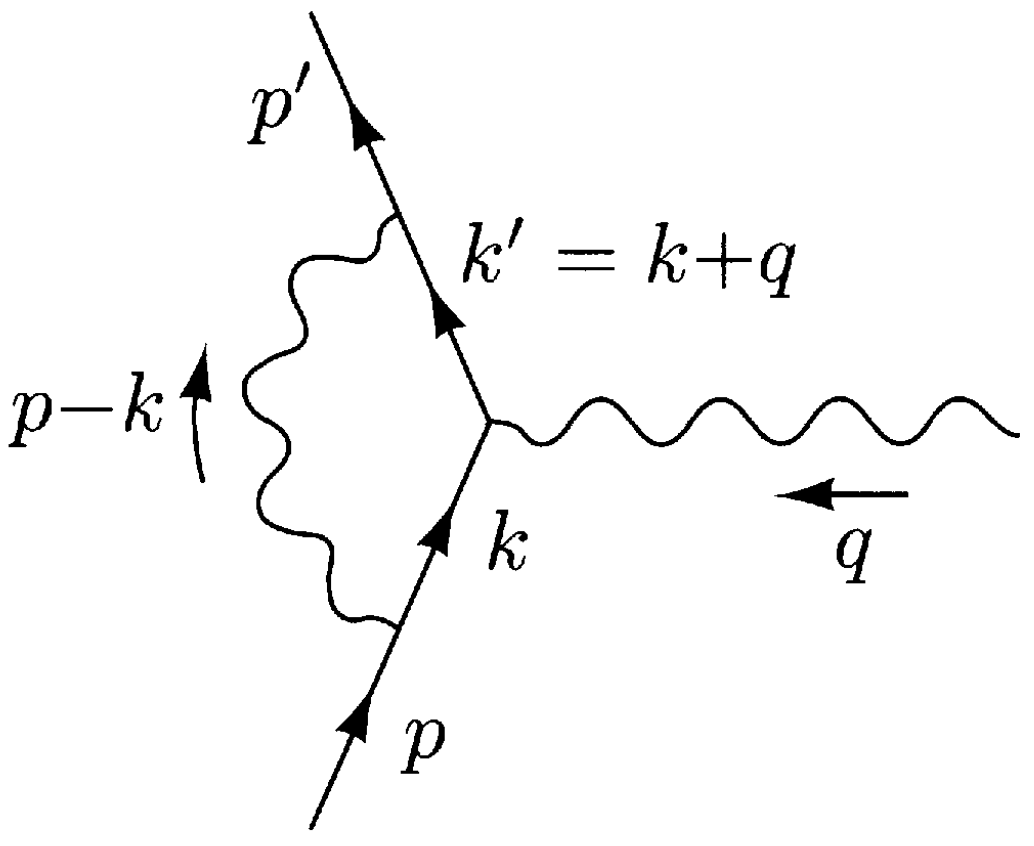
\includegraphics[width=0.3\linewidth]{pics/QED-3.png}
\end{equation*}
There is 4 electron propagator, 2 photon propagator, and 3 vertices.
Consider the perturbative expansion:
\begin{equation*}
	\frac{\delta^3}{i\delta J \delta\bar\eta \delta\eta}\frac{1}{2!}
	\left(\frac{-e\gamma^\mu_{\alpha\beta}\delta^3}{\delta J^\mu \delta\eta_{\alpha} \delta\bar\eta_{\beta}}\right)^3 
	\frac{1}{2!}\left(-i \bar\eta_{\alpha} D_F^{\alpha\beta} \eta_{\beta} \right)^4 
	\frac{1}{2!}\left(-\frac{i}{2} J^\mu \Pi_{\mu\nu} J^{\nu} \right)^2.
\end{equation*}
There is not symmetry factor, and an additional $-i$ factor. 
The total coefficient is $-ie^3$. 

Then consider the tensor contraction
\begin{equation*}
	D_F^{\alpha\gamma} \gamma^\nu_{\gamma\rho} D_F^{\rho\sigma} \gamma^\zeta_{\sigma\tau} D_F^{\tau\eta} \gamma^\lambda_{\eta\xi} D_F^{\xi\beta} \Pi_{\nu\lambda} \Pi_{\mu\zeta}.
\end{equation*}

The vertex correction is:
\begin{equation*}
	iV_3(q,p,p') = [iD_F(p)][iD_F(p')][i\Pi^{\mu\nu}(q)][-ie\Gamma^\nu(q,p,p')] 
\end{equation*}
where
\begin{equation}
	i\Gamma^\mu(q,p,p')
	= -e^2 \int\frac{d^4 k}{(2\pi)^4} 
	\Pi_{\nu\lambda}(p-k) 
	\gamma^\nu D_F(k') \gamma^\mu D_F(k) \gamma^\lambda.
	\label{eq:QED-loop-vertex}
\end{equation}
\end{framedexpl}

\begin{framedexpl}[Counter Terms]
Consider the counter term in the diagram
\begin{equation*}
	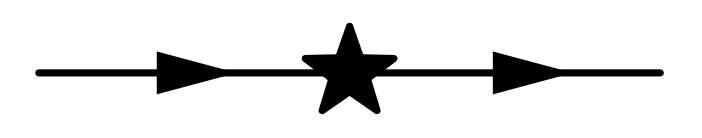
\includegraphics[width=0.25\linewidth]{pics/QED-ct-1.png}
\end{equation*}
The perturbative expansion is
\begin{equation*}
	iD_F^{\mathrm{(ct)}} \sim \frac{\delta^2}{\delta\bar\eta \delta\eta}
	i(\delta_{\psi}\gamma^\mu_{\alpha\beta}k_\mu-\delta_m \mathbb{I}_{\alpha\beta})\frac{\delta^2}{\delta\eta_{\alpha} \delta\bar\eta_{\beta}}
	\frac{1}{2!}\left(-i \bar\eta_{\alpha} D_F^{\alpha\beta} \eta_{\beta} \right)^2.
\end{equation*}
The contribution to the electron self energy is
\begin{equation*}
	\delta_{\psi}\cancel{k}-\delta_m m_R.
\end{equation*}
Similarly, the digram
\begin{equation*}
	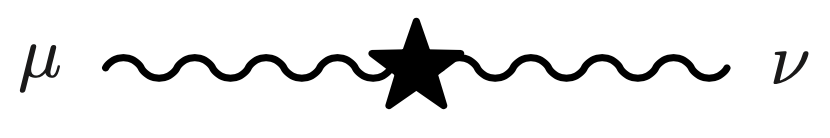
\includegraphics[width=0.25\linewidth]{pics/QED-ct-2.png}
\end{equation*}
contribute to the photon self energy with term
\begin{equation*}
	\delta_A [-p^2 g^{\mu\nu} + (1-\xi)p^\mu p^\nu],
\end{equation*}
and the diagram
\begin{equation*}
	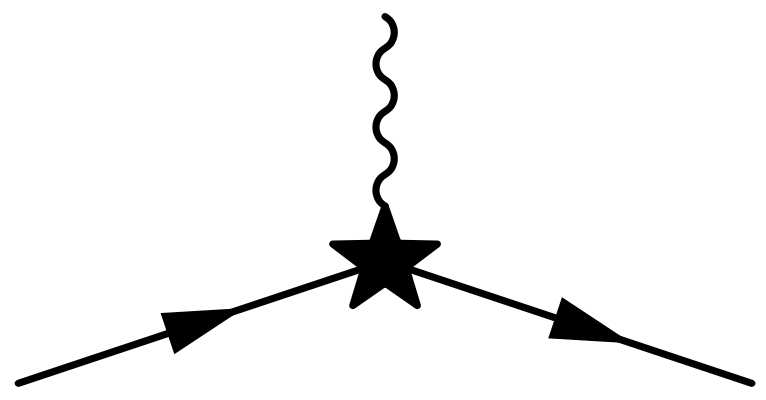
\includegraphics[width=0.2\linewidth]{pics/QED-ct-3.png}
\end{equation*}
contribute to the vertex with term
\begin{equation*}
	\delta_e \gamma^\mu.
\end{equation*}
\end{framedexpl}



\section{Loop Correction}
In this section, we consider the QED in ($d=4-\epsilon$) dimensional space-time.
\subsection{Electron Propagator}
Consider the one-loop correction to the electron propagator, where the self energy (\ref{eq:QED-ele-loop-prop}) is
\begin{equation}
\begin{aligned}
	i\Sigma(p^2)
	&= e^2\tilde{\mu}^{\epsilon}\int\frac{d^d k}{(2\pi)^d} \Pi_{\mu\nu}(p-k) \left[\gamma^\mu D_F(k) \gamma^\nu \right]_{\alpha\beta} \\
	&= -e^2\tilde{\mu}^{\epsilon}\int\frac{d^d k}{(2\pi)^d}\frac{\gamma^\mu(\cancel{k}+m)\gamma_\mu}{(p-k)^2(k^2-m^2)}.
\end{aligned}
\end{equation}
The nominator can be simplified using the \texttt{FeynCalc} Package:
\begin{lstlisting}[style=mathematicaFrameTB]
(*load FeynCalc Package*)
<< FeynCalc`

(*simplify the gamma expression*)
Contract[GA[\[Mu]].(GS[k]+m).GA[\[Mu]]]//DiracSimplify	
\end{lstlisting}
The result is
\begin{equation*}
	4 m-2\cancel{k}.
\end{equation*}
The denominator can be simplify using the Feynman parameter:
\begin{equation*}
	\frac{1}{(p-k)^2(k^2-m^2)} = \int_0^1 \frac{dx}{\left[(k-b)^2-D\right]^2}
\end{equation*}
where $b$ and $D$ can be calculated by
\begin{lstlisting}[style=mathematicaFrameTB]
A1=(k-p)^2;
A2=k^2-m^2;
{c,b,a}=CoefficientList[x*A1+(1-x)*A2,{k}];
-b/2
-c+b^2/(4*a)//Simplify
\end{lstlisting}
The result is
\begin{equation*}
	b = p x,\ 
	D = (1-x)(m^2-p^2 x).
\end{equation*}
Shift $k \rightarrow k + px$, the self energy becomes:
\begin{equation}
\begin{aligned}
	i\Sigma(p^2)
	&= 2e^2\tilde{\mu}^{\epsilon} 
		\int_0^1 (x\cancel{p}-2m)dx 
		\int \frac{d^d k}{(2\pi)^d} 
		\frac{1}{(k^2-D)^2} \\
	&= i\frac{2e^2 \tilde{\mu}^{\epsilon}\Omega_d}{(2\pi)^d}
		\int_0^1 (x\cancel{p}-2m)dx
		\int \frac{k^{d-1} dk}{(k^2+D)^2}.
\end{aligned}
\end{equation}
The regularization procedure
\begin{lstlisting}[style=mathematicaFrameTB]
omg=(2*Pi^(d/2))/(Gamma[d/2]);
cof=2*e^2*\[Mu]^(4-d)*omg/(2*Pi)^d;
int=cof*Integrate[q^(d-1)/(q^2+D)^2,{q,0,Infinity}][[1]];
map={e->Sqrt[4*Pi*\[Alpha]],EulerGamma->Subscript[\[Gamma],E]};
ans=Series[int/.{d->4-\[Epsilon]},{\[Epsilon],0,0}];
ans/.map//Simplify
\end{lstlisting}
The result is ($\mu^2 = 4\pi \tilde\mu^2 e^{-\gamma_E}$)
\begin{equation}
	\Sigma(p^2) = \frac{e_R^2}{8\pi^2}\int_0^1 dx(x\cancel{p}-2m_R)\left[\frac{2}{\epsilon}+\ln\left(\frac{\mu^2}{D}\right)\right].
\end{equation}
The infinity comes from
\begin{equation*}
	\frac{e_R^2}{4\pi^2\epsilon}\int_0^1 dx(x\cancel{p}-2m_R)
	= \frac{e_R^2}{8\pi^2\epsilon}\cancel{p} - \frac{e_R^2}{2\pi^2\epsilon}m_R.
\end{equation*}
Using the $\overline{\mathrm{MS}}$ subtraction scheme, we choose
\begin{equation}
	\delta_{\psi} = -\frac{e_R^2}{8\pi^2\epsilon},\ 
	\delta_m = -\frac{e_R^2}{2\pi^2\epsilon},
\end{equation}
and the self energy is
\begin{equation}
\begin{aligned}
	\Sigma(p^2) 
	&= \frac{e_R^2}{8\pi^2}\int_0^1 dx(x\cancel{p}-2m_R)\ln\left[\frac{\mu^2}{(1-x)(m_R^2-p^2 x)}\right] \\
	&= \frac{e_R^2}{8\pi^2}(\cancel{p}-4m_R)\ln\left(\frac{\mu}{m_R}\right)-\int_0^1 dx \ln\left[(1-x)\left(1-\frac{p^2x}{m_R^2}\right)\right].
\end{aligned}
\end{equation}



\subsection{Photon Self-energy}
Consider the one-loop correction to the photon propagator, where the self energy (\ref{eq:QED-photon-loop-prop}) is
\begin{equation}
	i \Sigma^{\mu\nu}
	= -e^2\tilde{\mu}^{\epsilon} \int\frac{d^d k}{(2\pi)^d} 
	\frac{\mathrm{Tr}\left[\gamma^\mu D_F(k-p) \gamma^\nu D_F(k) \right]}{(k^2-m^2)[(p-k)^2-m^2]}.
\end{equation}
The Dirac trace and Feynman parameter is calculated by
\begin{lstlisting}[style=mathematicaFrameTB]
(*Dirac trace*)
DiracTrace[GA[\[Mu]].(GS[k-p]+m).GA[\[Nu]].(GS[k]+m)]//DiracSimplify

(*Feynman paramater*)
A1=k^2-m^2;
A2=(k-p)^2-m^2;
{c,b,a}=CoefficientList[x*A1+(1-x)*A2,{k}];
-b/2
-c+b^2/(4*a)//Simplify
\end{lstlisting}
The nominator is
\begin{equation*}
	4 \left[g^{\mu\nu} \left(k\cdot p-{k}^2+m^2\right)+ 2k^\mu k^\nu - k^\mu p^\nu - p^\mu k^\nu \right]
\end{equation*}
The denominator is:
\begin{equation*}
	\frac{1}{(k^2-m^2)[(p-k)^2-m^2]}
	= \frac{1}{\left\{[k-p(1-x)]^2-[m^2+p^2 x(x-1)]\right\}^2}
\end{equation*}
Let $D=m^2-p^2 x(1-x)$, shift $k \rightarrow k + p(1-x)$, and drop all $p^\mu$ linear term,\footnote{The Ward identity requires that the $p^\mu$ term in the propagator do not contribute to any scattering process.} the result is
\begin{equation}
	i\Sigma^{\mu \nu}= -4 e^{2}\tilde{\mu}^{\epsilon} \int_0^1 dx
		\int \frac{d^{d} k}{(2 \pi)^{d}}  \frac{2 k^{\mu} k^{\nu}-g^{\mu \nu}\left[k^{2}-x(1-x) p^{2}-m^{2}\right]}{\left[k^{2}-D\right]^{2}}
\end{equation}
The self-energy $i\Sigma^\mu \propto g^{\mu\nu}$, we can make the substitution
\begin{equation*}
	k^\mu k^\nu \rightarrow \frac{1}{d} k^2 g^{\mu\nu}.
\end{equation*}
We then need to consider the integral
\begin{equation*}
\begin{aligned}
	iI(x) &= 4e^2\tilde{\mu}^{\epsilon} \int\frac{d^d k}{(2 \pi)^{d}}  
		\frac{(1-\frac{2}{d})k^{2}-x(1-x) p^{2}-m^{2}}{\left[k^{2}-D\right]^{2}}, \\
	I(x) &= -\frac{4e^2\tilde{\mu}^{\epsilon} \Omega_d }{(2\pi)^d}
		\int k^{d-1} dk \frac{(1-\frac{2}{d})k^{2}+x(1-x) p^{2}+m^{2}}{\left[k^{2}+D\right]^{2}}.
\end{aligned}
\end{equation*}
The regulation is carried out by the following code:
\begin{lstlisting}[style=mathematicaFrameTB]
omg=(2*Pi^(d/2))/(Gamma[d/2]);
cof=-4*e^2*\[Mu]^(4-d)*omg/(2*Pi)^d;
den=q^(d-1)*((1-2/d)q^2+x*(1-x)p^2+m^2);
int=cof*Integrate[den/(q^2+D)^2,{q,0,Infinity}][[1]];
map={EulerGamma->Subscript[\[Gamma],E],D->m^2-p^2*x*(1-x)};
ans=Series[int/.{d->4-\[Epsilon]},{\[Epsilon], 0, 0}];
ans/.map//Simplify
\end{lstlisting}
The result is
\begin{equation}
	\Sigma^{\mu\nu}(p^2) 
	= -\frac{e_R^2 p^2 g^{\mu\nu}}{2\pi^2} \int_0^1 dx\ x(1-x)
	\left[\frac{2}{\epsilon}+\ln\left(\frac{\mu^2}{m_R^2-p^2 x(1-x)}\right)\right]
\end{equation}
The divergent part is
\begin{equation*}
	-\frac{e_R^2 p^2 g^{\mu\nu}}{\pi^2 \epsilon} \int_0^1 dx\ x(1-x)
	= -\frac{e_R^2 p^2 g^{\mu\nu}}{6\pi^2 \epsilon}.
\end{equation*}
The counter term coefficient is
\begin{equation}
	\delta_A = -\frac{e_R^2}{6\pi^2 \epsilon}.
\end{equation}
The photon self-energy is then
\begin{equation}
\begin{aligned}
	\Sigma^{\mu\nu}(p^2) 
	&= -\frac{e_R^2 p^2 g^{\mu\nu}}{2\pi^2} \int_0^1 dx\ x(1-x)
	\ln\left[\frac{\mu^2}{m_R^2-p^2 x(1-x)}\right] \\
	&= -\frac{e_R^2 p^2 g^{\mu\nu}}{12\pi^2} \ln\left(\frac{\mu}{m}\right)
	 + \frac{e_R^2 p^2 g^{\mu\nu}}{2\pi^2}\int_0^{1} dx\ x(1-x) \ln\left[1-\frac{p^2}{m_R^2}x(1-x)\right].
\end{aligned}
\end{equation}


\subsection{Vertex Correction}
Consider the loop correction (\ref{eq:QED-loop-vertex}):
\begin{equation}
	i \Gamma^\mu(p,q_1,q_2)
	= e^2\tilde{\mu}^{\epsilon} \int\frac{d^4 k}{(2\pi)^4} 
	\frac{\gamma^\nu(\cancel{k}'+m)\gamma^\mu (\cancel{k}+m)\gamma_\nu}{(k^2-m^2)(k'^2-m^2)(p-k)^2}.
\end{equation}
Using the following code
\begin{lstlisting}[style=mathematicaFrameTB]
(*numerator*)
den=Contract[GA[\[Nu]].(GS[kp]+m).GA[\[Mu]].(GS[k]+m).GA[\[Nu]]];
DiracSimplify[den]

(*Feynman parameter*)
A1=k^2-m^2;
A2=(k+q)^2-m^2;
A3=(p-k)^2;
{c,b,a}=CoefficientList[x*A1+y*A2+z*A3,{k}];
-b/2//Simplify
-c+b^2/4//Simplify
\end{lstlisting}
The numerator is
\begin{equation*}
	-2\cancel{k}\gamma^\mu\cancel{k}'-2m^2\gamma^\mu + 4m(k + k')^\mu.
\end{equation*}
The denominator is
\begin{equation*}
	\int \frac{dF_3}{[(k+yq-zp)^2-D]^3},
\end{equation*}
where 
\begin{equation*}
\begin{aligned}
	D &= (x+y)m^2 - z(1-z)p^2- y(1-y)q^2-2yzpq \\
	&=(x+y)m^2 - xy q^2- yz p'^2 - xz p^2.
\end{aligned}
\end{equation*}
Shift $k^\mu \rightarrow k^\mu + z q_1^\mu - y p^\mu$, throw away all terms with linear $k^\mu$, and replace $k^\mu k^\nu$ with $\frac{1}{d}k^2 g^{\mu\nu}$, the result is
\begin{equation*}
	\frac{4}{d}k^2\gamma^\mu  -2(-y \cancel{q}+z \cancel{p}) \gamma^{\mu}[(1-y) \cancel q+z \cancel p] +4 m^{2} \gamma^{\mu}-2 m\left[(1-2 y) q^{\mu}+2 z p^{\mu}\right].
\end{equation*}
Note that only the quadratic term is divergent. 
\begin{equation*}
	\Gamma^\mu(p,q_1,q_2) = -i\frac{4e^2\tilde{\mu}^{\epsilon} \gamma^\mu}{d}  \int dF_3 \int \frac{d^dk}{(2\pi)^d} \frac{k^2}{(k^2-D)^3} + \delta\Gamma^\mu(p,q_1,q_2).
\end{equation*}
where $\delta \Gamma^\mu$ stores all the finite part
\begin{equation*}
\begin{aligned}
	& \delta\Gamma^\mu(p,q_1,q_2) \\
	=& \int \frac{e^2 k^3 dk dF_3}{(2\pi)^2(k^2+D)^3} \left\{(-y \cancel{q}+z \cancel{p}) \gamma^{\mu}[(1-y) \cancel q+z \cancel p] -2 m^{2} \gamma^{\mu}+ m\left[(1-2 y) q^{\mu}+2 z p^{\mu}\right]\right\}.
\end{aligned}
\end{equation*}
The divergent part is
\begin{equation*}
	\frac{4 e^2\tilde{\mu}^{\epsilon} \Omega_d \gamma^\mu}{d(2\pi)^d}\int dF_3 \int \frac{k^{d+1}dk}{(k^2+D)^3}
	= \frac{e_R^2}{16\pi^2} \gamma^\mu \int dF_3 \left[\frac{2}{\epsilon}+\ln\left(\frac{\mu^2}{D}\right)\right].
\end{equation*}
Using the $\overline{\mathrm{MS}}$ scheme, the coefficient of the counter term is
\begin{equation}
	\delta_e = -\frac{e_R^2}{8\pi^2\epsilon}.
\end{equation}


\subsection{Renormalization Group}
In summery, the renormalization factors are
\begin{equation}
\begin{aligned}
	Z_\psi &= 1 -\frac{e_R^2}{8\pi^2\epsilon} + O(e_R^3), \\
	Z_A &= 1 - \frac{e_R^2}{6\pi^2 \epsilon} + O(e_R^3), \\
	Z_m &= 1 - \frac{e_R^2}{2\pi^2\epsilon} + O(e_R^3), \\
	Z_e &= 1 - \frac{e_R^2}{8\pi^2\epsilon} + O(e_R^3),
\end{aligned}
\end{equation}
which means
\begin{equation}
\begin{aligned}
	\frac{d\ln Z_\phi}{d e_R} &= -\frac{e_R}{4\pi^2 \epsilon} + O(e_R^2), \\
	\frac{d\ln Z_A}{d e_R} &= -\frac{e_R}{3\pi^2 \epsilon} + O(e_R^2), \\
	\frac{d\ln Z_m}{d e_R} &= -\frac{e_R}{\pi^2 \epsilon} + O(e_R^2), \\
	\frac{d\ln Z_e}{d e_R} &= -\frac{e_R}{4\pi^2 \epsilon} + O(e_R^2).
\end{aligned}
\end{equation}
The bare parameters are
\begin{equation}
\begin{aligned}
	\psi_0 &= Z_\psi^{1/2}\psi_R, \\
	A_0 &= Z_A^{1/2} A_R, \\
	m_0 &= Z_m Z_\psi^{-1} m_R, \\
	e_0 &= Z_e Z_\psi^{-1} Z_A^{-1/2} e_R \tilde{\mu}^{\epsilon/2}. 
\end{aligned}
\end{equation}
The RG equation for $e_0$ is
\begin{equation}
	\frac{d\ln e_0}{d\ln \mu}
	= \left(\frac{\ln Z_e}{d e_R} - \frac{\ln Z_\psi}{d e_R} - \frac{1}{2} \frac{\ln Z_A}{d e_R} + \frac{1}{e_R} \right)\frac{de_R}{d\ln \mu} + \frac{\epsilon}{2} = 0.
\end{equation}
The beta function is
\begin{equation}
	\beta(e_R) = \frac{de_R}{d\ln \mu} = -\frac{\epsilon}{2}e_R + \frac{e_R^3}{12\pi^2} + O(e_R^4).
\end{equation}
The RG equation for $m_0$ is
\begin{equation}
	\frac{d\ln m_0}{d\ln \mu}
	= \left(\frac{\ln Z_m}{d e_R} - \frac{\ln Z_\psi}{d e_R}\right)\frac{de_R}{d\ln \mu} + + \frac{1}{m_R}\frac{d m_R}{d\ln\mu} = 0.
\end{equation}
The anomalous dimension of mass is
\begin{equation}
	\gamma_m = \frac{d \ln m_R}{d\ln\mu} = -\frac{3e_R^2}{8\pi^2} + O(e_R^3).
\end{equation}




\chapter{The Standard Model}

\section{Structure of the Standard Model}

The standard model (SM) describes all the elementary particles experimentally observed up till now.
It includes the electromagnetic, weak, and strong interactions, mediated by corresponding gauge fields.
Also, there is an additional scalar Higgs field in SM that gives masses to fermions and W, Z gauge bosons.


\subsection{Elementary Particles}

The elementary particles in SM can be divided into the fermions, the gauge bosons, and the Higgs boson. 
The fermions described the matters, the gauge boson mediate forces, and the Higgs couples to the matter and gauge field to create masses.

\begin{equation*}
	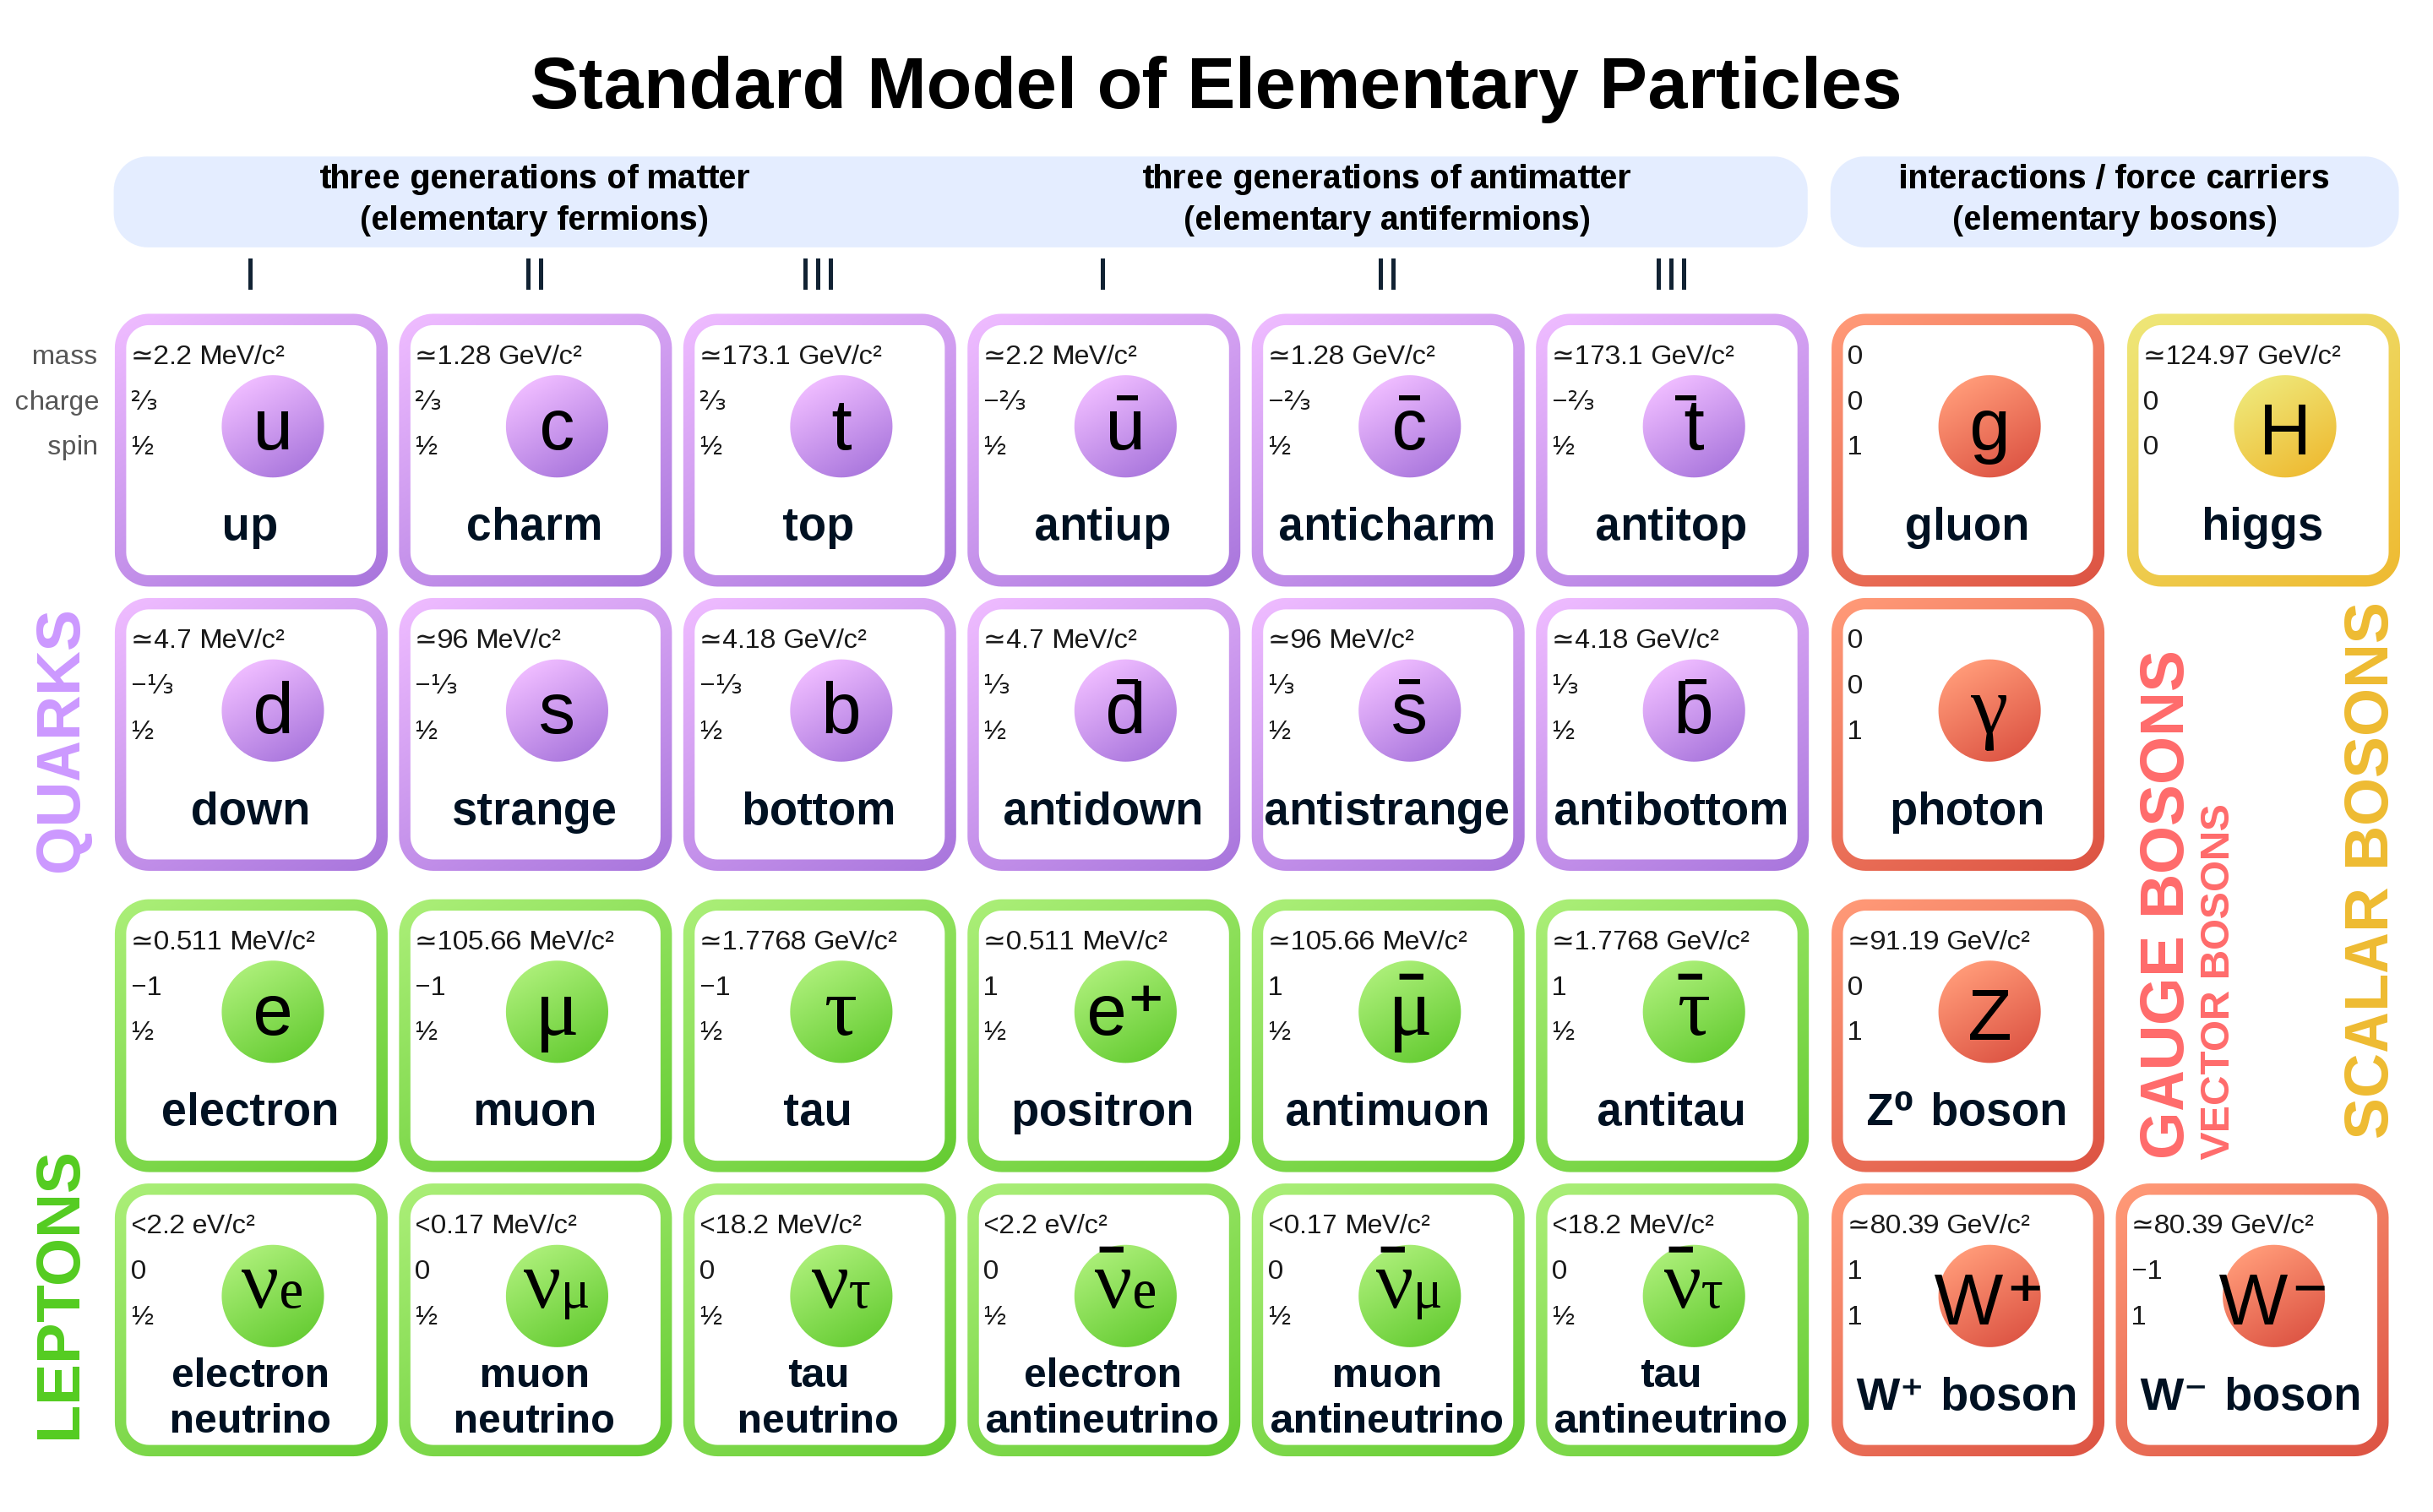
\includegraphics[width=0.8\linewidth]{pics/SM-Particles.png}
\end{equation*}

Composite particles like nucleons (neutron/proton) and mesons (pion, kaon, etc.) consist of quarks, which comes in six flavors: up, down, charm, strange, top, and bottom, and can also be grouped into three generations.
Besides, electrons and neutrinos are known as the lepton, which also comes in three generations.

The gauge bosons mediate electromagnetic force are the photons; for the weak interaction, they are the $W^\pm$ and $Z$ bosons, and for the strong force they are gluons, which comes in 8 colors.





\subsection{Gauge Group}

The standard model has $\mathrm{SU(3)}\times\mathrm{SU(2)}\times\mathrm{U(1)}$ gauge symmetry.
For a general field $\phi_{iI}$, where $i$ labels the electroweak degrees of freedom and $I$ labels the color degrees of freedom.
The covariant derivative for $\phi_{iI}$ is then
\begin{equation}
	D_\mu = \partial_\mu -i \left(g_1 B_\mu Y + g_2 W^a_\mu T^a_{2} + g_3 A_\mu^b T^b_3                                                  \right),
\end{equation}
where the operator $Y$, $T_2^a$ and $T_3^b$ is depend on the representation of U(1), SU(2) and SU(3) groups respectively. 

The weak interaction only involve left-handed spinor, so the largest fermion sector is
\begin{equation}
	Q_I = \left[
		\begin{pmatrix} u_L \\ d_L \end{pmatrix} 
		\begin{pmatrix} c_L \\ s_L \end{pmatrix} 
		\begin{pmatrix} t_L \\ b_L \end{pmatrix}
	\right]_I.
\end{equation}
Each $Q_I$ is in the $\left(3,2,\frac{1}{6}\right)$ representation, where $3$ is the fundamental representation of SU(3), $2$ is the fundamental representation of SU(2), and $\frac{1}{6}$ is the hypercharge of the U(1) gauge group.
For example the sector of first generation left-handed quarks are
\begin{equation}
	Q_1 = \begin{bmatrix}
		u_L^r & u_L^g & u_L^y \\ d_L^r & d_L^g & d_L^y
	\end{bmatrix}.
\end{equation}
Note that the electric charge satisfies $q = I_3 + Y$, where $I_3$ is the z-component of the isospin.

Besides, the left-handed leptons also involves the weak interaction but not the strong interaction
\begin{equation}
	L_I = \left[
		\begin{pmatrix} \nu_{e L} \\ e_L \end{pmatrix} 
		\begin{pmatrix} \nu_{\mu L} \\ \mu_L \end{pmatrix} 
		\begin{pmatrix} \nu_{\tau L} \\ \tau_L \end{pmatrix}
	\right]_I,
\end{equation}
and thus each $L_I$ is in the $\left(1,2,\frac{1}{2}\right)$ representation.

The right-handed quarks form $\left(3,1,\frac{2}{3}\right)$ and $\left(3,1,-\frac{1}{3}\right)$ representations, the right-handed electrons/muons/tauons form $\left(1,1,-1\right)$ representations, and the right-handed neutrinos form trivial $\left(1,1,0\right)$ representations.

In addition to the fermion, there is also a scalar Higgs field in the representation $\left(1,2,\frac{1}{2}\right)$.
Together, we say that the standard model contains the representations (only fermions in the first generation are listed):
\begin{equation}
\begin{tabular}{c|c|c}
\hline \hline
\multicolumn{2}{c|}{Particles} & Representation\tabularnewline
\hline 
\multirow{3}{*}{Quarks} & $Q_{1}$ & $(3,2,1/6)$\tabularnewline
 & $u_{R}$ & $(3,1,2/3)$\tabularnewline
 & $d_{R}$ & $(3,1,-1/3)$\tabularnewline
\hline 
\multirow{3}{*}{Leptons} & $L_{1}$ & $(1,2,-1/2)$\tabularnewline
 & $e_{R}$ & $(1,1,-1)$\tabularnewline
 & $\nu_{eR}$ & $(1,1,0)$\tabularnewline
\hline 
Higgs & $\varphi$ & $(1,2,1/2)$\tabularnewline
\hline \hline
\end{tabular}
\end{equation}

The standard model described the interaction of quarks, leptons and gauge bosons.
The gauge boson intermediate electromagnetic, weak, and strong interaction.
In the standard model, the gauge group is 
\begin{equation}
	G = \mathrm{SU(3)}\times \mathrm{SU(2)} \times \mathrm{U(1)},
\end{equation}
where $\mathrm{SU(3)}$ concerns the color degrees of freedom, and the $\mathrm{SU(2)}\times \mathrm{U(1)}$ is gauge group of the electroweak interaction.

The gauge field is coupled to the matter fields consists of 12 elementary fermion particles and a Higgs boson.

The gauge theory is written as a nonabelian gauge theory, or the Yang-Mills theory, which forbid the gauge field to have mass term.
Also, the weak interaction breaks the parity -- it only involve the left-handed spinor field, and such single-handed gauge symmetry forbid the mass term for fermions.
In order to obtain the mass, the Higgs field should be introduced, which involves the spontaneous symmetry breaking.


\subsection{Interactions}
The Lagrangian of the SM consists of
\begin{equation}
	\mathcal L_{\mathrm{SM}} = \mathcal L_{\mathrm{QED}} + \mathcal L_{\mathrm{QCD}} + \mathcal L_{\mathrm{W}} + \mathcal L_{\mathrm{H}}.
\end{equation}
In each sector, the free theory is described by the free fermions fields, free scalar fields or free vector fields.
The interaction among them can be represented by the Feynman diagrams.\footnote{All Feynman diagrams in the model are built from combinations of these vertices.The conjugate of each listed vertex (reversing the direction of arrows) is also allowed.}

The strong interaction involves the vertices:
\begin{equation}
	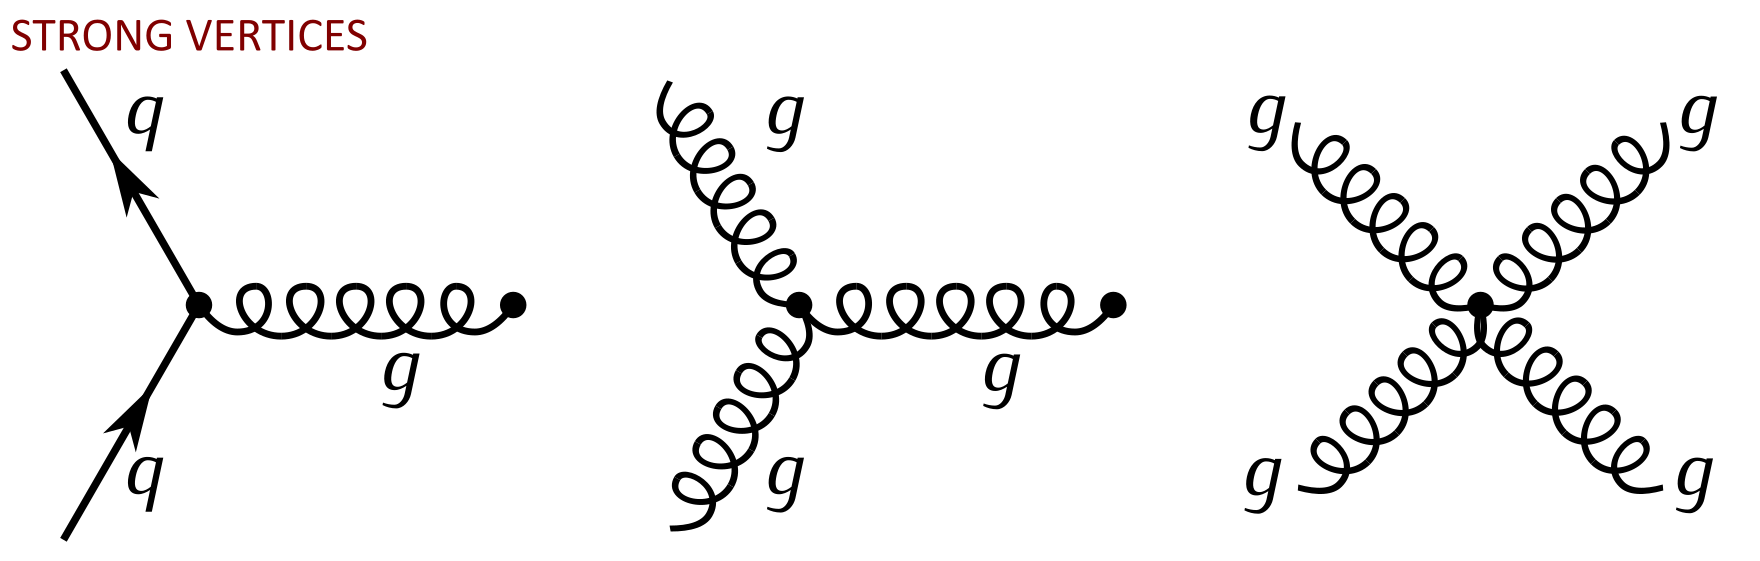
\includegraphics[width=0.5\linewidth,align=c]{pics/SM-Feyn-Strong.png}
\end{equation}
where $q$ is any quark, $g$ is a gluon.
The weak interaction involves the vertices:
\begin{equation}
	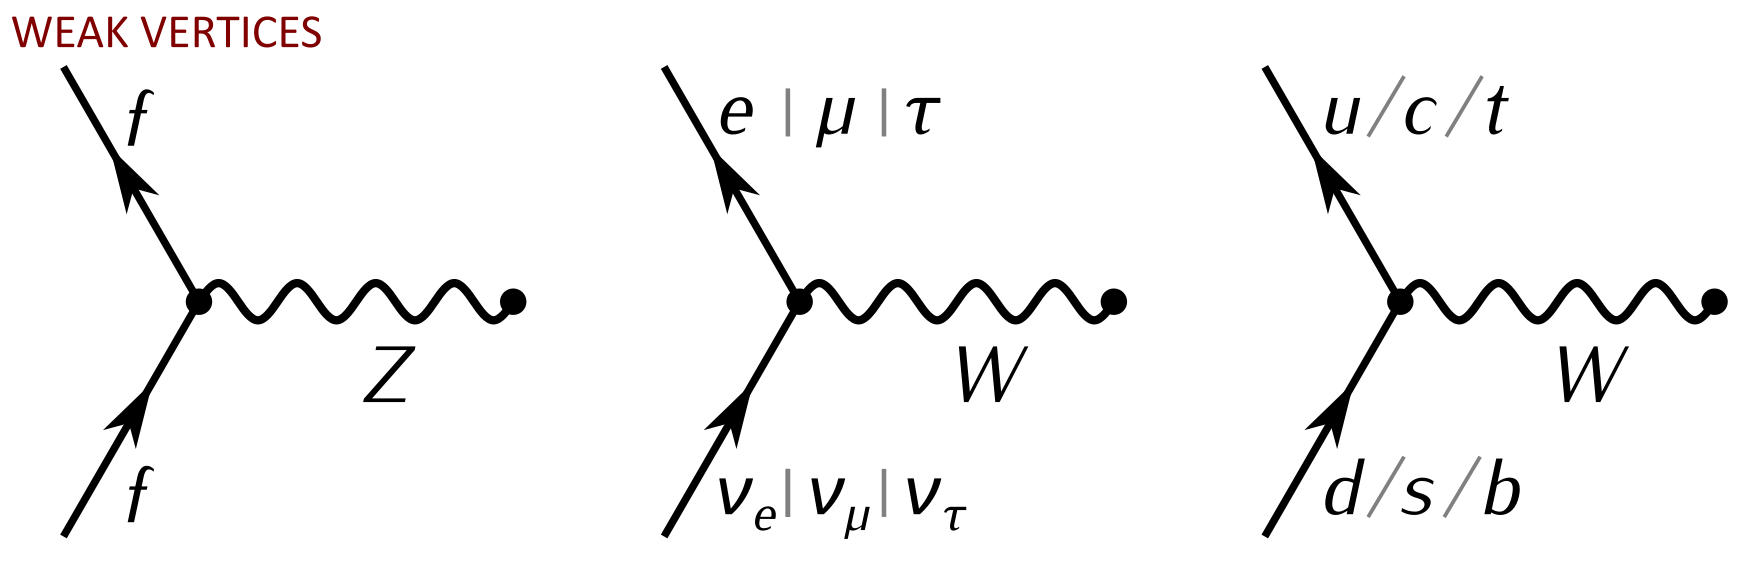
\includegraphics[width=0.5\linewidth,align=c]{pics/SM-Feyn-Weak.png}
\end{equation}
where $f$ is any fermion.

The electro-weak interaction involves the vertices:
\begin{equation}
	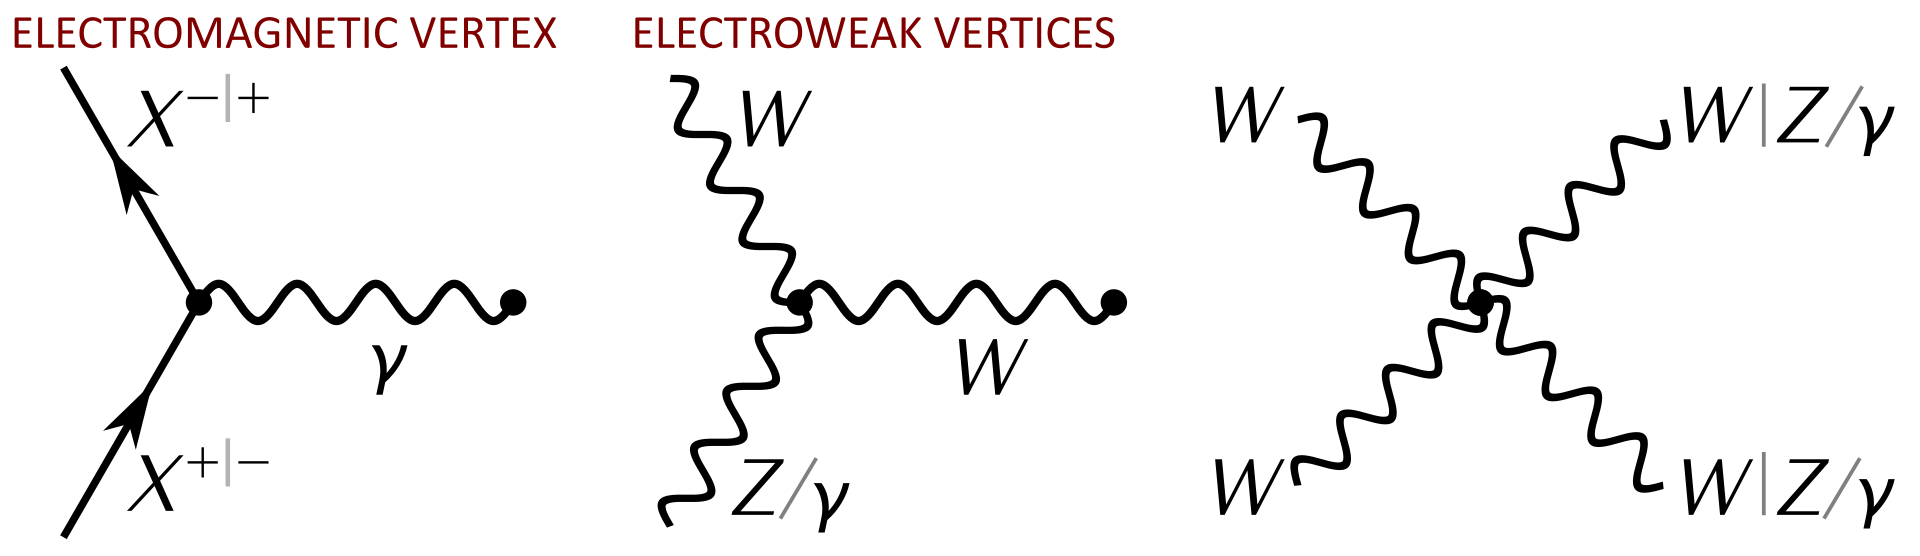
\includegraphics[width=0.5\linewidth,align=c]{pics/SM-Feyn-EW.png}
\end{equation}
where $X$ is any charged particle, $\gamma$ is a photon.
In diagrams with multiple particle labels separated by ``/'', one particle label is chosen. 
In diagrams with particle labels separated by ``|'', the labels must be chosen in the same order. 
For example, in the four boson electroweak case the valid diagrams are WWWW, WWZZ, WW$\gamma\gamma$, WWZ$\gamma$.

The Higgs vertices are:
\begin{equation}
	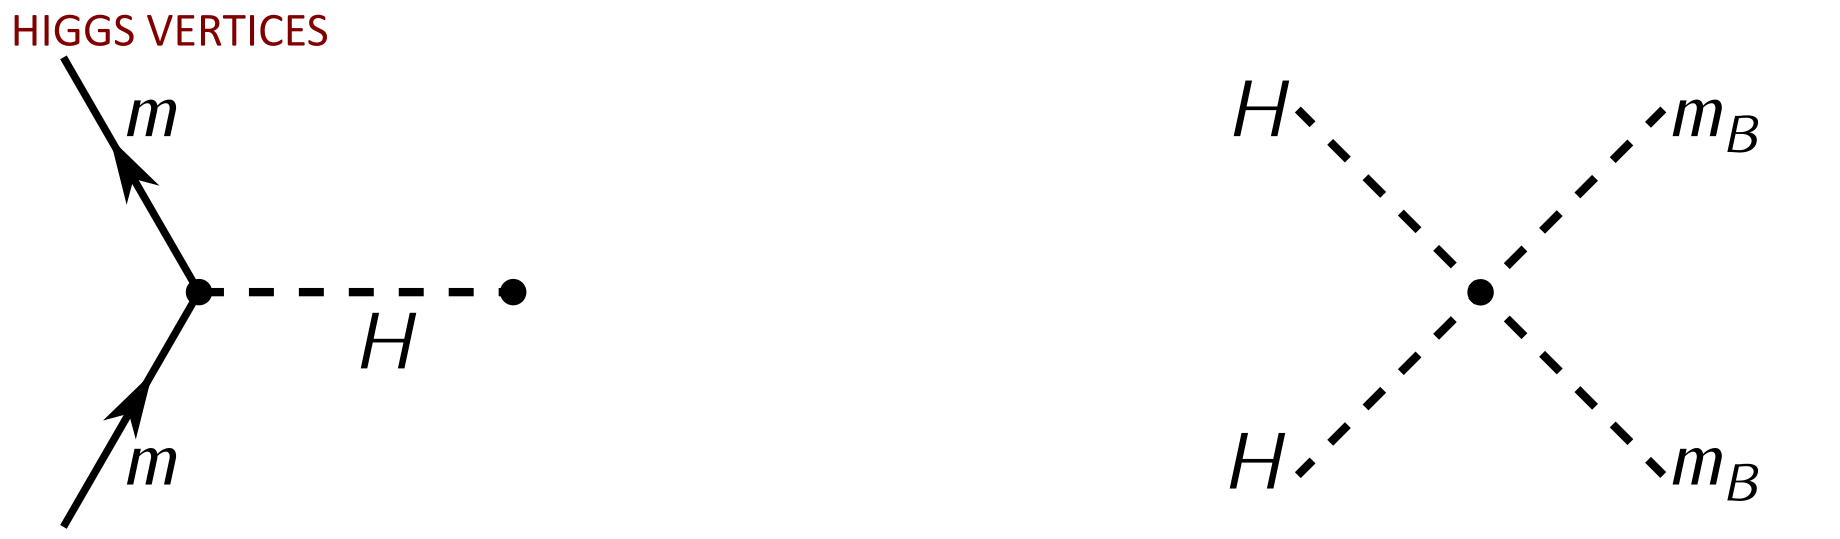
\includegraphics[width=0.5\linewidth,align=c]{pics/SM-Feyn-Higgs.png}
\end{equation}
where $m$ is any particle with mass, $m_B$ is any boson with mass. 
 








\section{Electroweak Interaction}

\subsection{Spontaneous Symmetry Breaking of Higgs Field}
Beside the quarks, leptons and gauge bosons, a doublet scalar field (Higgs) is also introduced in order to generate mass for the particles:
\begin{equation}
	\varphi \equiv \left[\begin{array}{c}
		\varphi_1 \\ \varphi_2
	\end{array} \right],
\end{equation}
which is also an isospin doublet with hyperchage $Y=\frac{1}{2}I$:
\begin{equation}
	\begin{tabular}{c c c c}
		\hline 
		Field & $I_3$ & $Y$ & $q$\\ \hline
		$\varphi_1$ & $1/2$ & $1/2$ & $1$ \\ 
		$\varphi_2$ & $-1/2$ & $1/2$ & $0$ \\  
		\hline 
	\end{tabular}
\end{equation}

The Lagrangian of the Higgs field is 
\begin{equation}\label{eq:SM-Higgs-L1}
	\mathcal L = -\frac{1}{4}(W^a_{\mu\nu})^2 - \frac{1}{4}B_{\mu\nu}^2 +(D^\mu \varphi)^\dagger D_\mu \varphi- V(\varphi),
\end{equation}
where the field strength tensors are
\begin{equation}
\begin{aligned}
	W^a_{\mu\nu} &= \partial_\mu W_\nu^1 - \partial_\nu W^1_\mu + g_2 (W_\mu^2 W_\nu^3 - W_\mu^3 W_\nu^2), \\
	W^a_{\mu\nu} &= \partial_\mu W_\nu^1 - \partial_\nu W^1_\mu + g_2 (W_\mu^3 W_\nu^1 - W_\mu^1 W_\nu^3), \\
	W^a_{\mu\nu} &= \partial_\mu W_\nu^1 - \partial_\nu W^1_\mu + g_2 (W_\mu^1 W_\nu^2 - W_\mu^2 W_\nu^1), \\
	B^a_{\mu\nu} &= \partial_\mu B_\nu^1 - \partial_\nu B^1_\mu,
\end{aligned}
\end{equation}
and the Higgs interaction is
\begin{equation}
	V(\varphi) = \frac{\lambda}{4} \left(\varphi^\dagger \varphi - \frac{v^2}{2} \right)^2.
\end{equation}
This potential gives $\varphi$ a nonzero vacuum expectation value (VEV). 
We can make a gauge transformation so that
\begin{equation}
	\varphi_0 = \langle 0| \varphi |0\rangle = \frac{v}{\sqrt 2} \left[\begin{array}{c}
		0 \\ 1	\end{array} \right].
\end{equation}


The kinetic Lagrangian is described by the SU(2) gauge-invariant Lagrangian
\begin{equation}
	\mathcal L_{\mathrm{kin}} = (D^\mu \varphi)^\dagger D_\mu \varphi,
\end{equation}
where the covariant derivative is
\begin{equation}
	D_\mu = \partial_\mu -i \left(g_1 B_\mu Y + g_2 W^a_\mu T_2^a\right).
\end{equation}
We can introducing the Weinberg angle
\begin{equation}
	\theta_W \equiv\arctan \frac{g_1}{g_2},
\end{equation}
and the fields
\begin{equation}
\begin{aligned}
	W_\mu^\pm &\equiv \frac{1}{\sqrt 2}(W^1_\mu \mp i A_\mu^2), \\
	Z_\mu &\equiv \cos{\theta_W} W^3_\mu - \sin{\theta_W} B_\mu, \\
	A_\mu &\equiv \sin{\theta_W} W_\mu^3 + \cos{\theta_W} B_\mu.
\end{aligned}
\end{equation}
The reverse transformation for $W_\mu^3$ and $B_\mu$ is
\begin{equation}
\begin{aligned}
	W_\mu^3 &= \cos{\theta_W} Z_\mu + \sin{\theta_W} A_\mu, \\
	B_\mu &= -\sin{\theta_W} Z_\mu +\cos{\theta_W} A_\mu.
\end{aligned}
\end{equation}
The off-diagonal part of the Lie algebra becomes
\begin{equation}
	\frac{1}{\sqrt 2}\begin{bmatrix}
		0 &  W^+_\mu \\
		W_\mu^- & 0
	\end{bmatrix},
\end{equation}
and the diagonal part becomes
\begin{equation}
\begin{aligned}
	g_2 W_\mu^3 T^z_2 + g_1 B_\mu Y
	&= g_2 (\cos{\theta_W} Z_\mu + \sin{\theta_W} A_\mu) T^3_2 + g_1 Y (-\sin{\theta_W} Z_\mu +\cos{\theta_W} A_\mu) \\
	&= g_2 \cos{\theta_W} A_\mu \left(T^3_2 + Y\right) + eZ_\mu \left(\cot{\theta_W}T_2^3 - \tan{\theta_W}Y \right) \\
	&= e A_\mu q + \frac{e}{\sin{\theta_W}\cos{\theta_W}} Z_\mu \left(\cos^2{\theta_W}T_2^3 - \sin^2{\theta_W} Y\right) \\
	&= e A_\mu q + \frac{e}{\sin{\theta_W}\cos{\theta_W}} Z_\mu \left(T_2^3 - \sin^2{\theta_W} q\right).
\end{aligned}
\end{equation}
Note that the gauge field $A_\mu$ describe QED, so we identify the coupling constant with the electric charge:
\begin{equation}
	e = g_2 \sin{\theta_W} = g_1 \cos{\theta_W}.
\end{equation}

For Higgs field, 
\begin{equation}
	T^3_2 = \frac{1}{2}\sigma^z, \quad
	Y = \frac{1}{2} I,\quad 
	q = \begin{bmatrix}
		1 & 0 \\ 0 & 0
	\end{bmatrix}.
\end{equation}
$T^3_2 = \frac{1}{2}\sigma^z$, $Y=\frac{1}{2}I$, so 
With the new definition of the field, the Lie algebra of becomes
\begin{equation}
\begin{aligned}
	g_2 W^a_\mu T_2^a + g_1 B_\mu Y 
	&= \frac{e}{2 \sin{\theta_W}} 
	\begin{bmatrix}
		2\sin{\theta_W} A_\mu + \frac{\cos{2\theta_W}}{\cos{\theta_W}} Z_\mu & \sqrt{2} W^+_\mu \\
		\sqrt{2} W_\mu^- & \frac{1}{\cos{\theta_W}} Z_\mu
	\end{bmatrix}.
\end{aligned}
\end{equation}
We can now expand the kinetic term to get the effective mass of the the gauge field in unitary gauge. 
The mass term is the quadratic part of $\varphi$:
\begin{equation}
\begin{aligned}
	\mathcal L_{\mathrm{mass}} 
	&= \varphi_0^\dagger \left(g_2 W^a_\mu T_2^a + g_1 B_\mu Y\right)^2 \varphi_0 \\
	&= \frac{e^2v^2}{8 \sin^2{\theta_W}} 
	\begin{bmatrix}
		0 & 1
	\end{bmatrix} 
	\begin{bmatrix}
		\cdots & \sqrt{2} W^+_\mu \\
		\sqrt{2} W_\mu^- & \frac{1}{\cos{\theta_W}} Z_\mu
	\end{bmatrix}^2
	\begin{bmatrix}
		0 \\ 1
	\end{bmatrix} \\
	&= m_W W^{+\mu} W_\mu^- + \frac{1}{2}m_Z^2 Z^\mu Z_\mu,
\end{aligned}
\end{equation}
where the mass for $W$ and $Z$ bosons are
\begin{equation}
	m_W = \frac{ev}{2 \sin{\theta_W}}, \quad 
	m_Z = \frac{e v}{2\sin{\theta_W}\cos{\theta_W}} = \frac{m_W}{\cos{\theta_W}}.
\end{equation}
Note that the photon field $A_\mu$ does not obtain mass from the Higgs field.



\subsection{Lagrangian of Higgs-Gauge Sector}
We are now going to express the Lagrangian (\ref{eq:SM-Higgs-L1}) in terms of the fields we have just introduced.
In the unitary gauge, the Higgs field can be written as
\begin{equation}
	\varphi = \frac{1}{\sqrt 2} \begin{bmatrix}
		v + H(x) \\ 0
	\end{bmatrix},
\end{equation}
where $H(x)$ is a real scalar field.
The interaction terms gives
\begin{equation}
\begin{aligned}
	V(H) &= \frac{\lambda v^2}{4} H^2 + \frac{\lambda v}{4}H^3 + \frac{\lambda}{16}H^4 \\
	&= \frac{1}{2}m_H^2 H^2 + \frac{m_H^2}{2v} H^3 + \frac{m_H^2}{8v^2}H^4,
\end{aligned} 
\end{equation}
where we have defined the Higgs mass
\begin{equation}
	m_H^2 = \frac{\lambda v^2}{2}.
\end{equation}
Also, the fluctuation around the $\varphi_0$ also create coupling between Higgs field and the gauge fields.
We can simply replace $v^2$ with $(v+H)^2$ in the gauge field mass term to capture the coupling.
Thus, the Lagrangian is
\begin{equation}
	\mathcal L_{\mathrm{H}} = \partial^\mu H^\dagger \partial_\mu H - V(H) + \left(m_W W^{+\mu} W_\mu^- + \frac{1}{2}m_Z^2 Z^\mu Z_\mu \right) \left(H^2+2vH \right).
\end{equation}
Now consider the Lagrangian for the gauge field
\begin{equation}
	\mathcal L_\mathrm{W} = -\frac{1}{4}(W^a_{\mu\nu})^2 - \frac{1}{4}B_{\mu\nu}^2 + m_W W^{+\mu} W_\mu^- + \frac{1}{2}m_Z^2 Z^\mu Z_\mu.
\end{equation}
We can regroup the field strength as
\begin{equation}
\begin{aligned}
	W^+_{\mu\nu} &= D_\mu W_\nu^+ - D_\nu W^+_\mu, \\
	W^-_{\mu\nu} &= D_\mu^\dagger W_\nu^- - D_\nu^\dagger W^-_\mu, \\
	W^3_{\mu\nu} &= \sin{\theta_W} F_{\mu\nu} + \cos{\theta_W}Z_{\mu\nu} -ig_2(W^+_\mu W^-_\nu - W_\mu^- W_\nu^+), \\
	B^a_{\mu\nu} &= \cos{\theta_W} F_{\mu\nu} - \sin{\theta_W} Z_{\mu\nu},
\end{aligned}
\end{equation}
where we have defined 
\begin{equation}
\begin{aligned}
	W^\pm_{\mu\nu} &= \frac{1}{\sqrt 2} (W^1_{\mu\nu} \mp i W^2_{\mu\nu}), \\
	F_{\mu\nu} &= \partial_\mu A_\nu - \partial_\nu A_\mu, \\
	Z_{\mu\nu} &= \partial_\mu Z_\nu - \partial_\nu Z_\mu.
\end{aligned}
\end{equation}
The covariant derivative for $W^\pm$ field is
\begin{equation}
\begin{aligned}
	D_\mu &= \partial_\mu -i g_2 W^3_\mu \\
	&= \partial_\mu -i g_2 \left(\sin{\theta_W}A_\mu + \cos{\theta_W} Z_\mu \right) \\
	&= \partial_\mu -i e \left(A_\mu + \cot{\theta_W} Z_\mu \right)
\end{aligned}
\end{equation}
So the Lagrangian for the gauge field is
\begin{equation}
\begin{aligned}
	\mathcal L_\mathrm{W}
	=&\ -\frac{1}{4}(2W_{\mu\nu}^+ W^{-\mu\nu} + W_{\mu\nu}^3 W^{3\mu\nu}) -\frac{1}{4} B_{\mu\nu}B^{\mu\nu} + m_W W^{+\mu} W_\mu^- + \frac{1}{2}m_Z^2 Z^\mu Z_\mu \\
	=&\ -\frac{1}{4}(F_{\mu\nu}F^{\mu\nu} + Z_{\mu\nu} Z^{\mu\nu}) - D^{\mu} W^{+\nu} D^\dagger_\mu W_\nu^- + D^\mu W^{+\nu} D^\dagger_\nu W^-_\mu \\
	&\ +ie (F^{\mu\nu} + \cot{\theta_W} Z^{\mu\nu})W_\mu^+ W_\nu^- + m_W W^{+\mu} W_\mu^- + \frac{1}{2}m_Z^2 Z^\mu Z_\mu \\
	&\ -\frac{e^2}{2\sin^2{\theta_W}} \left(W^{+\mu}W^-_\mu W^{+\nu}W^-_\nu - W^{+\mu}W^+_\mu W^{-\nu}W^-_\nu \right).
\end{aligned}
\end{equation}
We remark that in the unitary gauge, there is no redundancy of the gauge field.
No ghost field is needed in the quantization procedure.


\section{Yukawa Couplings}
The fermion fields in the electroweak interaction
\begin{equation}
	\begin{tabular}{c c c c}
		\hline 
		Field & $I_3$ & $Y$ & $q$\\ \hline
		$u_L$ & $1/2$ & $1/6$ & $2/3$ \\ 
		$d_L$ & $-1/2$ & $1/6$ & $-1/3$ \\  
		$u_R$ & $0$ & $2/3$ & $2/3$ \\
		$d_R$ & $0$ & $-1/3$ & $-1/3$ \\ \hline
		$e_L$ & $-1/2$ & $-1/2$ & $-1$ \\ 
		$\nu_{eL}$ & $1/2$ & $-1/2$ & $0$ \\  
		$e_R$ & $0$ & $-1$ & $-1$ \\
		$\nu_{eR}$ & $0$ & $0$ & $0$ \\
		\hline 
	\end{tabular}
\end{equation}

The kinetic term for the fermion Lagrangian is
\begin{equation}
\begin{aligned}
	\mathcal L_{\mathrm{kin}}
	=&\ i Q^\dagger_J \sigma^\mu D_\mu Q_J + i u_{RJ}^\dagger \bar\sigma^\mu D_\mu u_{RJ} + i d_{RJ}^\dagger \bar\sigma^\mu D_\mu d_{RJ} \\
	& + i L^\dagger_J \sigma^\mu D_\mu L_J + i e_{RJ}^\dagger \bar\sigma^\mu D_\mu e_{RJ} + i \nu_{RJ}^\dagger \bar\sigma^\mu D_\mu \nu_{RJ},
\end{aligned}
\end{equation}
where we have use the index $J$ to label the generation of the fermion:
\begin{equation}
\begin{aligned}
	u_{RJ} &= \{u_R, c_R, t_R\}, & 
	d_{RJ} &= \{d_R, s_R, b_R\}, \\
	e_{RJ} &= \{e_R, \mu_R, \tau_R\}, &
	\nu_{RJ} &= \{\nu_{eR},\nu_{\mu R},\nu_{\tau R}\}.
\end{aligned}
\end{equation}

The left-handed SU(2) gauge symmetry forbid any fermion mass term, which is incompatible with the reality.
However, fermion can obtain fermion mass by introducing Yukawa coupling between the Higgs and fermion fields.

\subsection{Quark Sector}
The Yukawa coupling between quark and Higgs is
\begin{equation}
	\mathcal L_{q,\mathrm{Yuk}}
	= - \varepsilon^{ij} Y^u_{IJ} Q^\dagger_{iI} \varphi^\dagger_j u_{RJ}
	- Y^d_{IJ} Q^\dagger_{I} \varphi d_{RJ} +h.c..
\end{equation}
The first term corresponds to
\begin{equation}
	\left(\bar 3, \bar 2, -\frac{1}{6}\right) \times \left(1, \bar 2, -\frac{1}{2}\right) \times \left(3, 1, \frac{2}{3}\right) = \left(1,1,0\right)\oplus \cdots,
\end{equation}
with $\varepsilon^{ij}$ being the Clebsch-Gordan coefficient, and the second term corresponds to
\begin{equation}
	\left(\bar 3, \bar 2, -\frac{1}{6}\right) \times \left(1, 2, \frac{1}{2}\right) \times \left(3, 1, -\frac{1}{3}\right) = \left(1,1,0\right).
\end{equation}
Now substitute $\varphi$ with 
\begin{equation}
	\varphi = \frac{1}{\sqrt 2} \begin{bmatrix}
		0 \\ v+H
	\end{bmatrix}.
\end{equation}
The Yukawa potential then gives quark mass term:
\begin{equation}
	\mathcal L_{Q,\mathrm{Yuk}}
	= -\frac{v+H}{\sqrt 2} \left( Y^u_{IJ} u^\dagger_{LI} u_{RJ} +Y^d_{IJ} d^\dagger_{LI} d_{RJ} \right) +h.c..
\end{equation}
We can then use a basis transformation (singular value decomposition) to diagonalize the coupling matrix:
\begin{equation}
	Y^u_{IJ} = U_u M_u K^\dagger_u, \quad
	Y^d_{IJ} = U_d M_d K^\dagger_d,
\end{equation}
where $M_u$ and $M_d$ are diagonal matrices.
We can change the basis
\begin{equation}
\begin{aligned}
	u_L &\rightarrow U_u u_L, & u_R &\rightarrow K_u u_R, \\
	d_L &\rightarrow U_d d_L, & d_R &\rightarrow K_d d_R,
\end{aligned}
\end{equation}
and define the diagonal masses:
\begin{equation}
	m_{u_I} = \frac{v}{\sqrt 2} (M_u)_{II}, \quad 
	m_{d_I} = \frac{v}{\sqrt 2} (M_d)_{II},
\end{equation}
then the Lagrangian in the quark sector can be expressed as:
\begin{equation}
\begin{aligned}
	\mathcal L_Q =&\ \sum_I \bar u_I\left(i\cancel D^c-m_{u_I}\right)u_I + \sum_I \bar d_I \left(i \cancel D^c-m_{d_I}\right)d_I \\
	& -\frac{H}{v} \sum_I\left(m_{u_I}\bar u_I u_I+m_{d_I}\bar d_I d_I \right) + \mathcal L_{Q-G},
\end{aligned}
\end{equation}
where $\cancel D^c$ is the covariant derivative in QCD (neglecting the electroweak gauge), and $\mathcal L_{Q-G}$ denotes the coupling between quarks and the gauge fields.
Using the expression of the Lie algebra
\begin{equation}
\begin{aligned}
	g_2 \sum_{a=1}^2 W^a_\mu T^a_2 &= \frac{e}{\sqrt{2}\sin{\theta_W}}\begin{bmatrix}
		0 & W_\mu^+ \\ W_\mu^- & 0
	\end{bmatrix}, \\
	g_2 W_\mu^3 T^z_2 + g_1 B_\mu Y
	&= e A_\mu q + \frac{e}{\sin{\theta_W}\cos{\theta_W}} Z_\mu \left(T_2^3 - \sin^2{\theta_W} q\right),
\end{aligned}
\end{equation}
The gauge-current coupling is:
\begin{equation}
	\mathcal L_{Q-G} = \frac{e}{\sqrt{2}\sin{\theta_W}} \left(W^{+}_\mu J_Q^{+\mu} + W^{-}_\mu J_Q^{-\mu} \right) + e A_\mu J^{\mu}_{\mathrm{EM},Q} + \frac{e}{\sin{\theta_W}\cos{\theta_W}} Z_\mu J^\mu_{z,Q},
\end{equation}
where the currents are defined as
\begin{equation}
\begin{aligned}
	J^{+\mu}_Q &= d_{LI}^\dagger \bar\sigma^\mu u_{LI}, \quad
	J^{-\mu}_Q = u_{LI}^\dagger \bar\sigma^\mu d_{LI}, \\
	J^\mu_{\mathrm{EM},Q} &= \frac{2}{3} u_{LI}^\dagger \bar\sigma^\mu u_{LI} - \frac{1}{3} d_{LI}^\dagger \bar\sigma^\mu d_{LI}, \\
	J_{z,Q}^\mu &= \frac{1}{2} u_{LI}^\dagger \bar\sigma^\mu u_{LI} - \frac{1}{2} d_{LI}^\dagger \bar\sigma^\mu d_{LI} J^\mu_3-\sin^2{\theta_W}J_{\mathrm{EM},Q}^\mu.
\end{aligned}
\end{equation}
We note that in the definition of the currents, the quarks is the eigenstates of the weak interaction, not the mass eigenstates.
If we define the quarks as the particle with definite mass, the above definition shall be rotation by a unitary matrix.


\subsection{Lepton Sector}
The coupling between Higgs and $e_R$ has the general Yukawa form:
\begin{equation}
	\mathcal L_{e,\mathrm{Yuk}} = -Y^e_{IJ} L_{iI}^\dagger \varphi_j e_{R iJ} + h.c.,
\end{equation}
where $y_{IJ}$ is the Hermitian coupling matrix on generation space.
The Yukawa coupling term corresponds to
\begin{equation}
	\left(\bar 2, \frac{1}{2}\right) \times \left(2, \frac{1}{2}\right) \times \left(1, -1\right) = \left(1,0\right),
\end{equation}
which is indeed a singlet under gauge transformation (it is also a singlet under Lorentz transformation).
The Higgs field then produce the term
\begin{equation}
	\mathcal L_{e,\mathrm{Yuk}} = -\frac{Y^e_{IJ}}{\sqrt 2}(v+H) e_{LI}^\dagger e_{RJ} + h.c.,
\end{equation}
We then diagonalize the coupling matrix:
\begin{equation}
	 Y^e_{IJ} = \left[U_{e} M_e K^\dagger_{e}\right]_{IJ},
\end{equation}
where $M_e$ is diagonal.
We can then change the basis by
\begin{equation}
\begin{aligned}
	e_R &\rightarrow K_e e_R, \\
	e_L &\rightarrow U_e e_L,
\end{aligned}
\end{equation}
Then the coupling gives the mass:
\begin{equation}
	\mathcal L_{e,\mathrm{Yuk}} 
	= - \sum_I m_{e_I} \bar e_I e_I - \frac{H}{v}\sum_I m_{e_I} \bar e_I e_I,
\end{equation}
where
\begin{equation}
	m_{e_I} = \frac{v}{\sqrt 2} (M_e)_{II}.
\end{equation}

Now we consider the neutrino mass, which is much smaller than electrons.
The neutrinos can similarly obtain mass by coupling to Higgs field.
However, as the neutrinos being charge neutral, the mass term can come from Yukawa coupling as well as the Majorana pairing:
\begin{equation}
\begin{aligned}
	\mathcal L_{\nu,\mathrm{Yuk}} 
	&= - Y^\nu_{IJ} \varepsilon^{ij} L_{iI} \varphi_j \nu_{RJ} - \frac{1}{2} M_{IJ} \nu_{RI} \cdot \nu_{RJ} + h.c. \\
	&= -\frac{Y^\nu_{IJ}}{\sqrt 2}(v+H) \nu_{LI}^\dagger \nu_{RJ} - \frac{1}{2}M_{IJ}\nu_{RI}\cdot \nu_{RJ} + h.c.
\end{aligned}
\end{equation}
The first term corresponds to
\begin{equation}
	\left(2, -\frac{1}{2}\right) \times \left(2, \frac{1}{2}\right) \times \left(1, 0\right) = \left(1,0\right) \oplus(3,0),
\end{equation}
and $\varepsilon^{ij}$ is the Clebsch-Gordan coefficients.
The second term is automatically a gauge singlet.
We can make a basis change to make $Y$ diagonal, and define a new set of Dirac spinors from single Weyl spinors:
\begin{equation}
	\psi_1 = \begin{pmatrix}
		\nu_L \\ i\sigma^2 \nu_L^*
	\end{pmatrix}, \quad
	\psi_2 = \begin{pmatrix}
		-i\sigma^2 \nu_R^* \\ \nu_R
	\end{pmatrix},
\end{equation}
and the effective mass term can be written as:
\begin{equation}
	\mathcal L_{\nu,\mathrm{mass}} 
	= -\sum_I \frac{Y_{II} v}{\sqrt 2}\bar\psi_{1I} \psi_{2I} - \sum_{IJ}\frac{1}{2} M_{IJ} \bar\psi_{2I} \psi_{2J}.
\end{equation}
Now the Dirac spinor $\psi_1$ and $\psi_2$ can mix, and a suitable mixing renders the mass term diagonal.
If $M \gg m$, the eigenvalues of the mass term will be a huge masses plus some tiny masses.
In general, the low-energy part of the mass term is
\begin{equation}
	\mathcal L_{\nu,\mathrm{mass}} = -\sum_I m_{\nu_I}\bar\nu_I \nu_I \left(1+\frac{H}{v}\right)^2,
\end{equation}

With the discussion above, we can write down the Lagrangian in the lepton sector:
\begin{equation}
\begin{aligned}
	\mathcal L_L =&\ \sum_I \bar e_I (i\cancel\partial-m_{e_I})e_I + \sum_I \nu_{LI}^\dagger (\bar\sigma^\mu \partial_\mu -m_{\nu_I})\nu_{LI} \\
	& -\frac{H}{v} \sum_I \left(m_{e_I} \bar e_I e_I + m_{\nu_I}\bar\nu_{LI}\nu_{LI}\right)+ \mathcal L_{L-G},
\end{aligned}
\end{equation}
where $\mathcal L_{L-G}$ is the lepton-gauge coupling term:
\begin{equation}
	\mathcal L_{L-G} = \frac{e}{\sqrt{2}\sin{\theta_W}}\left(W^{+}_\mu J_L^{+\mu} + W^{-}_\mu J_L^{-\mu} \right) + e A_\mu J^{\mu}_{\mathrm{EM},L} + \frac{e}{\sin{\theta_W}\cos{\theta_W}} Z_\mu J^\mu_{z,L},
\end{equation}
where the current is defined as 
\begin{equation}
\begin{aligned}
	J^{+\mu}_L &= e_{LI}^\dagger \bar\sigma^\mu \nu_{LJ}, \\
	J^{-\mu}_L &= \nu_{LI}^\dagger \bar\sigma^\mu e_{LJ}, \\
	J^\mu_{\mathrm{EM},L} &= - e_{LI}^\dagger \bar\sigma^\mu e_{LI} \\
	J_{z,L}^\mu &= \frac{1}{2} \nu_{LI}^\dagger \bar\sigma^\mu \nu_{LI} - \frac{1}{2} e_{LI}^\dagger \bar\sigma^\mu e_{LI} J^\mu_3-\sin^2{\theta_W}J_{\mathrm{EM},L}^\mu.
\end{aligned}
\end{equation}
We note that although right-handed neutrinos are introduced, experimentally we can only directly observe the left-handed neutrinos.
For the same reason the eigenstate of the weak interaction works more natural than the mass eigenstate for neutrinos. 
We choose to define the neutrinos as what we directly measured -- the left-handed ``particle'' with no definite mass.



\subsection{Particle Mixing}

\subsubsection{Quark Mixing}
In the above discussion, when talking about ``particles'', we actually mean two different things. 
The original definition of the particle is an excitation with definite energy.
But in the weak interaction process, say
\begin{equation}
	u \rightarrow d + W^+,
\end{equation}
the strange and charm quark is the eigenstate of the weak interaction.
That is, the weak interaction can change a state called $u$ to a states called $d$, both of which not necessarily have fixed energies.
If we stick to the original definition of the particles, it turns out that the isospin doublet $Q_I$ we have just defined is not exact.
It really should be written as
\begin{equation}
	Q_I = \left[
		\begin{pmatrix} u_L' \\ d_L' \end{pmatrix},
		\begin{pmatrix} c_L' \\ s_L' \end{pmatrix},
		\begin{pmatrix} t_L' \\ b_L' \end{pmatrix}
	\right],
\end{equation}
where the primed quarks are mixtures of particle quarks from three generations.
Without the loss of generality, we can identify $u'=u$, $c'=c$, $t'=t$, the mixing of quarks happens for the remaining three flavors:
\begin{equation}
	\begin{pmatrix}
		d' \\ s' \\ b'
	\end{pmatrix}
	= \begin{bmatrix}
		V_{ud} & V_{us} & V_{ub} \\
		V_{cd} & V_{cs} & V_{cb} \\
		V_{td} & V_{ts} & V_{tb}
	\end{bmatrix}
	\begin{pmatrix}
		d \\ s \\ b.
	\end{pmatrix}
\end{equation}
The matrix $V$, being unitary, is called the \textit{Cabbibo-Kobayashi-Maskawa} (CKM) matrix.
From the calculation above, we know
\begin{equation}
	V \equiv U^\dagger_u U_d.
\end{equation}
The quark mixing changes the original definition of $J^\pm_Q$ to:
\begin{equation}
\begin{aligned}
	J^{+\mu}_Q &= {d'}_{LI}^{\dagger} \bar\sigma^\mu u_{LI}
		= V^\dagger_{IJ} d_{LI}^\dagger \bar\sigma^\mu u_{LJ}, \\
	J^{-\mu}_Q &= u_{LI}^\dagger \bar\sigma^\mu d'_{LI}
		= V_{IJ} u_{LI}^\dagger \bar\sigma^\mu d_{LJ}.
\end{aligned}
\end{equation}
Note that the diagonal current $J_{\mathrm{EM}}$ or $J_z$ will not change change under the basis transformation.

The experimental value of the CKM matrix is approximately
\begin{equation}
	\begin{bmatrix}
		\left|V_{u d}\right| & \left|V_{u s}\right| & \left|V_{u b}\right| \\
		\left|V_{c d}\right| & \left|V_{c s}\right| & \left|V_{c b}\right| \\
		\left|V_{t d}\right| & \left|V_{t s}\right| & \left|V_{t b}\right|
	\end{bmatrix} =
	\begin{bmatrix}
		0.97 & 0.22 & 0.004 \\
		0.22 & 0.97 & 0.04 \\
		0.009 & 0.04 & 0.999
	\end{bmatrix}.
\end{equation}
We see the CKM matrix is closed to an identity matrix, and the most mixing happens between $d$ and $s$ quarks, i.e.,
\begin{equation}
\begin{aligned}
	d' &= \cos\theta_c\ d + \sin\theta_c\ s \\
	s' &= -\sin\theta_c\ d + \cos\theta_c\ s.
\end{aligned}
\end{equation}
Here the angle $\theta_c \approx 13^{\circ}$ is called the Cabbibo angle.
It correct the quark decay process to:
\begin{equation}
	\left[u \rightarrow d' + W^+\right]
	= \cos\theta_c \left[u \rightarrow d + W^+\right] + \sin\theta_c \left[u \rightarrow s + W^+\right].
\end{equation}


\subsubsection{Neutrino Oscillation}
Quite similarly, particles in lepton sector also mix.
We choose to identify $e'_L = e_L$ (similarly for muon and tauon).
Neutrinos that have specific mass are called $\nu_1$, $\nu_2$, and $\nu_3$ instead, which satisfies
\begin{equation}
	\begin{pmatrix}
		\nu_{e} \\ \nu_{\mu} \\ \nu_{\tau}
	\end{pmatrix} = 
	\begin{bmatrix}
		U_{e 1} & U_{e 2} & U_{e 3} \\
		U_{\mu 1} & U_{\mu 2} & U_{\mu 3} \\
		U_{\tau 1} & U_{\tau 2} & U_{\tau 3}
	\end{bmatrix}
	\begin{pmatrix}
		\nu_{1} \\ \nu_{2} \\ \nu_{3}
	\end{pmatrix},
\end{equation}
the $3 \times 3$ matrix is known as the \textit{Pontecorvo-Maki-Nakagawa-Sakata} (PMNS) matrix, or simply the neutrino mixing matrix.
Its value is roughly
\begin{equation}
	\begin{bmatrix}
		\left|U_{e 1}\right|\left|U_{e 2}\right|\left|U_{e 3}\right| \\
		\left|U_{\mu 1}\right|\left|U_{\mu 2}\right|\left|U_{\mu 3}\right| \\
		\left|U_{\tau 1}\right|\left|U_{\tau 2}\right|\left|U_{\tau 3}\right|
	\end{bmatrix} \approx
	\begin{bmatrix}
		0.8 & 0.5 & 0.1 \\
		0.3 & 0.5 & 0.7 \\
		0.4 & 0.6 & 0.6
	\end{bmatrix}.
\end{equation}
The neutrino mixing means that in the weak process, say
\begin{equation}
	e \rightarrow \nu_e + W^-,
\end{equation}
the produced neutrino $\nu_e$ is not an energy eigenstate of the SM Hamiltonian -- it will oscillates.
As for the definition of the lepton current $J^\pm_L$. 
If we stick to the definition of neutrino as the eigenstate of the weak interaction -- since that is what we get from the particle decay process -- we do not need to change the definition, but we should remember that such ``neutrinos'' do not have fixed mass.


\subsubsection{Restore 4-Fermion Theory}
Finally, we can sum over the current, and write down the total fermion-gauge coupling:
\begin{equation}
	\mathcal L_{F-G} = \frac{e}{\sqrt{2}\sin{\theta_W}} \left(W^{+}_\mu J^{+\mu} + W^{-}_\mu J^{-\mu} \right) + e A_\mu J^{\mu}_{\mathrm{EM}} + \frac{e}{\sin{\theta_W}\cos{\theta_W}} Z_\mu J^\mu_{z}.
\end{equation}
From the current-gauge coupling, we can recover the effective 4-fermion theory by integrating out the gauge field.
In the low energy regime ($p^2 \ll m_W^2$), the vertex function for electron decay is:
\begin{equation}
	2\left(\frac{e}{\sqrt{2}\sin{\theta_W}} \right)^2 J^+_\mu \frac{g^{\mu\nu}}{p^2-m_W^2} J^-_\nu 
	\simeq \frac{e^2}{m_W^2 \sin^2{\theta_W}} J^{+\mu} J^-_\mu.
\end{equation}
The diagonal part of the vertex is
\begin{equation}
	\left(\frac{e}{\sin{\theta_W}\cos{\theta_W}} \right)^2 J^z_\mu \frac{g^{\mu\nu}}{p^2-m_Z^2} J^z_\nu 
	\simeq -\frac{e^2}{m_Z^2 \sin^2{\theta_W}\cos^2{\theta_W}} J^{z\mu} J^z_\mu.
\end{equation}\
Note that $m_Z^2\cos^2{\theta_W} = m_W^2$, we can then identify the fermion constant
\begin{equation}
	\frac{4G_F}{\sqrt 2} = -\frac{e^2}{m_W^2 \sin^2{\theta_W}},
\end{equation}
and the 4-Fermion vertex is
\begin{equation}
	\mathcal L_{4F} = -\frac{4G_F}{\sqrt 2} \left(J^{+\mu} J_\mu^- + J^{z\mu} J_\mu^z \right).
\end{equation}

















\chapter{Lattice Systems}

\section{Lattice Spins}

\subsection{The Ising Model}
The Ising model on the Euclidean space is described by the action
\begin{equation}
	S[\{s_k\}] = -K \sum_{\langle ij\rangle} s_i s_j,\quad s_k = \pm 1.
\end{equation}
where $\langle ij \rangle$ is the nearest-neighbor sites and the coupling is
\begin{equation}
	K = \beta J = \frac{J}{T}.
\end{equation}
The phase of the Ising model can be revealed by considering the correlation function:
\begin{equation}
	G_{ij} \equiv \langle \sigma_i^z \sigma_j^z\rangle
	= \frac{1}{Z} \sum_{\{s_k\}} e^{-S[\{s_k\}]} s_i s_j,
\end{equation}
where the partition function is
\begin{equation}
	Z = \sum_{\{s_k\}} e^{-S[\{s_k\}]}
\end{equation}


\subsubsection{Series Expansion}
The behavior of correlation in the high- and low- temperature limit can be seen using the series expansion.
Consider first the high-temperature limit where $K \rightarrow 0$, the partition function can be expanded in different order of $K$:
\begin{equation}
\begin{aligned}
	Z &= \sum_{\{s_k\}} \prod_{\langle ij\rangle} \cosh K (1 + s_i s_j \tanh K) \\
	&\sim \sum_{\{s_k\}} \prod_{\langle ij\rangle} (1 + s_i s_j K).
\end{aligned}
\end{equation}
The only terms that survive the averaging form a non-crossing path from site $i$ to site $j$.
In the small $K$ limit, the main contribution comes from the shortest path, i.e.,
\begin{equation}
	G_{ij} \propto K^{-r_{ij}},
\end{equation}
where $r_{ij}$ is the distance (Manhattan metric) from $i$ to $j$.
We see in high temperature the correlation is exponentially decaying, indicating a disorder phase.
Note that for $d=1$ case, there is only one path from $i$ to $j$, and the exact result is
\begin{equation}
	G_{ij} = \frac{(2\cosh K \tanh K)^{|i-j|}}{(2 \cosh K)^{|i-j|}}
	= \left(\tanh K\right)^{|i-j|},
\end{equation}
independent of the temperature, so the 1d Ising model has only one phase.

For $d\ge 2$ case, in the lower temperature limit, the dominant contribution to the partition function comes from the ferromagnetic configuration.
The excitations are the spin domains, whose energy is proportional to their perimeters.
For higher dimensional system, the creation of the domain is suppressed, leading to an ordered phase.



\section{Lattice Fermions}
In this section, we consider the system whose Hamiltonian composed of quadratic fermionic operators, i.e.,
\begin{equation}
	\hat H_{\mathrm{free}} = \sum_{i,j=1}^N A_{ij} c_i^\dagger c_j + \frac{1}{2}\sum_{i,j=1}^N B_{ij} c_i c_j + \frac{1}{2}\sum_{i,j=1}^N B_{ij}^* c_j^\dagger c_i^\dagger, \label{eq:lattice-free-fermion-hamiltonian}
\end{equation}
where $A$ is a Hermitian matrix, and matrix $B$ is anti-symmetric.
Without loss of generality, in the following we always assume that the sum of chemical potential is zero, i.e., $\mathrm{Tr} A=0$.
In the Nambu basis 
\begin{equation}
	\Psi = (c_1,\dots,c_N,c_1^\dagger,\dots,c_N^\dagger)^T,
\end{equation}
the Hamiltonian has the BdG form:
\begin{equation}
	\hat H_{\mathrm{free}} = \frac{1}{2} \sum_{i,j=1}^{2N} \Psi^\dagger_i H_{ij}^{\Psi} \Psi_j + \frac{1}{2}\mathrm{Tr}A,
\end{equation}
where the single-body matrix $H^{\Psi}$ is a $2N\times 2N$ Hermitian matrix
\begin{equation}
	H^{\Psi} = \left[\begin{array}{cc} 
		A & B \\
		-B^* & -A^* 
	\end{array}\right].
\end{equation}
Note that in the Nambu basis, the single-body Hamiltonian matrix has the particle-hole symmetry
\begin{equation}
	P = \sigma_x \mathcal K, 
	\quad \Longrightarrow \quad
	P H^{\Psi} P = -H^{\Psi}.
\end{equation}
This means the spectrum of the BdG Hamiltonian is symmetric with respect to zero.


\subsection{Majorana Representation}

The Majorana operators are defined as:
\begin{equation}
	\left[\begin{array}{c} \omega_{i} \\ \omega_{i+N} \end{array}\right]
	= \left[\begin{array}{cc} 
		1 & 1 \\ 
		i & -i 
	\end{array}\right] \left[\begin{array}{c} 
		c_i \\ c_i^\dagger 
	\end{array}\right], \quad 
	\left[\begin{array}{c} c_i \\ c_i^\dagger \end{array}\right]
	= \frac{1}{2} \left[\begin{array}{cc} 
		1 & -i \\ 
		1 & i 
	\end{array}\right] \left[\begin{array}{c} 
		\omega_{i} \\ \omega_{i+N}
	\end{array}\right].
\end{equation}
The Majorana operator satisfies the Fermion-like commutation relation
\begin{equation}
	\{\omega_i, \omega_j\} = 2\delta_{ij}.
\end{equation}
The fermionic bilinear in the Majorana basis has the form
\begin{equation}
	\hat H = -\frac{i}{4} \sum_{i,j=1}^{2N} H_{ij} \omega_i \omega_j
\end{equation}
where the single-body matrix $H$ is a $2N \times 2N$ real anti-symmetric matrix:
\begin{equation}
	H = \left[\begin{array}{cc} 
		-A^I - B^I & A^R - B^R \\
    	-A^R - B^R &  -A^I + B^I 
	\end{array}\right].
\end{equation}
where we have define $A^{R/I} = \mathrm{Re} A / \mathrm{Im} A$ and $B^{R/I} = \mathrm{Re} B / \mathrm{Im} B$.
Conversely, if we have a Majorana bilinear 
\begin{equation}
	\frac{i}{2} \sum_{i,j=1}^{2N} M_{ij}\omega_i \omega_j, \quad
	M = \left[\begin{array}{cc}
		M^{11} & M^{12} \\ M^{21} & M^{22}
	\end{array} \right],
\end{equation}
it can be transformed back to ordinary fermionic bilinear (\ref{eq:lattice-free-fermion-hamiltonian}) where
\begin{equation}
\begin{aligned}
	A &= M^{21} - M^{12} + i M^{11} + i M^{22}, \\
	B &= M^{21} + M^{12} + i M^{11} - i M^{22}.
	\label{eq:lattice-majorana-bilinear-to-fermion}
\end{aligned}
\end{equation}
A real anti-symmetric matrix can be transformed to standard form by an orthogonal transformation $O$:
\begin{equation}
\begin{aligned}
	H &= O \cdot \Sigma(\bm \lambda) \cdot O^T, \\
	\Sigma(\bm \lambda) &= i\sigma_y \otimes \mathrm{diag}(\lambda_1,\cdots,\lambda_n).
\end{aligned}
\end{equation}
Make the basis transformation
\begin{equation}
	\gamma_n = \sum_{j=1}^{2N} O_{jn} \omega_j,
\end{equation}
the Hamiltonian becomes the standard form:
\begin{equation}
\begin{aligned}
	H &= -\frac{i}{4} \sum_{i=1}^N \lambda_i (\gamma_i \gamma_{i+N}-\gamma_{i+N} \gamma_i) \\
	&= -\frac{i}{2} \sum_{i=1}^N \lambda_i \gamma_i \gamma_{i+N}.
\end{aligned}
\end{equation}
Each $\gamma_i \gamma_{i+N}$ pair can then transforms to independent fermion mode:
\begin{equation}
\begin{aligned}
	-\frac{i}{2}\gamma_i \gamma_{i+N} 
	&= -\frac{i}{2}(d_i + d_i^\dagger)(id_i-id_i^\dagger) \\ 
	&= d_i^\dagger d_i-\frac{1}{2}.
\end{aligned}
\end{equation}



\subsection{Gaussian States}
The Fermionic Gaussian states are those states with Gaussian form density operator:
\begin{equation}
	\hat \rho \propto \exp \left(\frac{i}{2}\sum_{i,j=1}^{2N}M_{ij}\omega_i \omega_j \right),
\end{equation}
where the matrix $M$ is real and anti-symmetric.\footnote{In particular, any thermal state has this form, with $M = \beta H/2$. The ground state of the free fermion system, though being pure state, can be regarded as the Gaussian state in the limit $M = \lim_{\beta \rightarrow \infty} \beta H$.}
If we expand the Gaussian form, the density operator becomes a Majorana polynomial:\footnote{Note that the coefficient $\Gamma$ in each order is not the direct expansion of the matrix $M$, since the direct expansion contains identical Majorana operators. That is, the $n$-th order expansion of the Majorana Gaussian form may contribute to the ($n-2m$)-th order term in the Majorana polynomial.}
\begin{equation}
	\hat{\rho} = \frac{\mathbb{I}}{2^N} + \sum_{n=1}^{N}\frac{i^n}{2^N}\sum_{1\le i_{1}<\cdots<i_{2n} \le 2N}\Gamma_{i_{1}\cdots i_{2n}} \omega_{i_1}\cdots\omega_{i_{2n}},
\end{equation}
where the coefficient $\Gamma_{i_1 \cdots i_{2n}}$ is the $2n$-point correlation function:
\begin{equation}
	\Gamma_{i_1 \cdots i_{2n}} = i^n \langle \omega_{i_1} \cdots \omega_{i_{2n}}\rangle, \quad i_m \ne i_n.
\end{equation}
In particular, the 2-point function 
\begin{equation}
	\Gamma_{ij} = i\langle \omega_i \omega_j\rangle - i\delta_{ij} = \frac{i}{2}\langle [\omega_i, \omega_j]\rangle
\end{equation}
is also called the \textit{covariance matrix}. 
For Gaussian state all $2n$-point correlation is determined by the covariance matrix by the Wick theorem.
\begin{framedrmk}[Two-point Correlation Function]
We are usually more familiar with the ordinary fermionic two-point correlation function $\langle c^\dagger_i c_j\rangle$ or $\langle c_i c_j\rangle$, which is related to the Majorana covariance matrix by:
\begin{equation}
\begin{aligned}
	\langle c_i^\dagger c_j\rangle &= \frac{1}{4}(
		\Gamma^{21}_{ij} - \Gamma^{12}_{ij} + 
		i \Gamma^{11}_{ij} + i \Gamma^{22}_{ij})
		+\frac{1}{2}\mathbb \delta_{ij}, \\
	\langle c_i c_j\rangle &= \frac{1}{4}(
		\Gamma^{21}_{ij} + \Gamma^{12}_{ij} + 
		i \Gamma^{11}_{ij} - i \Gamma^{22}_{ij}), \\
	\langle c_i^\dagger c_j^\dagger\rangle &= \frac{1}{4}(
		-\Gamma^{21}_{ij} - \Gamma^{12}_{ij} + 
		i \Gamma^{11}_{ij} - i \Gamma^{22}_{ij}).
\end{aligned}
\end{equation}
\end{framedrmk}

The relation of the correlation in each order can be neatly captured by the Grassmannian Gaussian form:
\begin{equation}
\begin{aligned}
	\omega(\hat \rho, \theta) 
	&= \frac{1}{2^N} \exp \left(\frac{i}{2} \sum_{i,j=1}^{2N}\Gamma_{ij}\theta_i \theta_j \right) \\
	&=\frac{1}{2^N} + \sum_{n=1}^{N}\frac{i^n}{2^N}\sum_{1\le i_{1}<\cdots<i_{2n} \le 2N}\Gamma_{i_{1}\cdots i_{2n}} \theta_{i_1} \cdots \theta_{i_{2n}}.
\end{aligned}
\end{equation}
When the covariance matrix is obtained, we can use the same routine to canonicalize the skew-symmetric matrix $\Gamma$:
\begin{equation*}
	\Gamma = O \cdot \Sigma(\bm \lambda) \cdot O^T, \quad
	\tilde\theta_n = \sum_i O_{in} \theta_i,
\end{equation*}
and the density matrix in the Grassmann representation is
\begin{equation}
	\omega(\hat \rho, \theta) 
	= \prod_{n=1}^N \left(\frac{1}{2} e^{i \lambda_n \tilde\theta_n \tilde\theta_{n+N}} \right)
	= \prod_{n=1}^N \left(\frac{1+i\lambda_n \tilde\theta_n\tilde\theta_{n+N}}{2}  \right).
\end{equation}
This state correspond to a product state $\rho = \otimes_n \rho_n$ where
\begin{equation}
	\rho_n = \frac{1}{2} \left[\begin{array}{cc}
		1 + \lambda_n & 0 \\
		0 & 1 - \lambda_n
	\end{array} \right].
\end{equation}
The entanglement entropy is then
\begin{equation}
	S=\sum_n S_n = -\sum_n \left[
	\left(\frac{1+\lambda_n}{2}\right)\ln\left(\frac{1+\lambda_n}{2}\right)
	+ \left(\frac{1-\lambda_n}{2}\right)\ln\left(\frac{1-\lambda_n}{2}\right)\right].
\end{equation}


\subsection{Jordan-Wigner Transformation}
Some lattice spin model can be mapped to fermion one by the Jordan-Wigner (J-W) transformation, which defines the isomorphism between the fermion and spin Hilbert space.
One a single site, we map the 




\section{Lattice Gauges}




\chapter{Non-relativistic Quantum Field Theory}
A general non-relativistic field theory is described by the action (with repeated indices automatically summed):
\begin{equation}
\begin{aligned}
	S &= S_0 + S_{\mathrm{int}} = \int dt \int d^d x \mathcal{L}_0 + \int dt\ \mathcal{V}_{\mathrm{int}}, \\
	\mathcal{L}_0 &= \bar\psi_a(x) (i\delta_{ab}\partial_t-\hat H_{ab})\psi_b(x).
\end{aligned}
\end{equation}
where the field operator $\psi(x)$ can be bosonic or fermionic, which is denoted by a number $\zeta=\pm 1$, and $\mathcal{V}_{\mathrm{int}}$ is the interaction Lagrangian.
A general interaction has the form
\begin{equation}
	\mathcal{V}_{\mathrm{int}} = \sum_{abcd}\int \prod_{i=1}^4 d^d x_i \ \bar\psi_{c}(x_3)\bar\psi_{d}(x_4) V_{abcd}(x_1,x_2,x_3,x_4) \psi_{b}(x_2)\psi_{a}(x_1).
\end{equation}
Note that the classical equation of motion for the free field satisfies the Schr\"{o}dinger equation:
\begin{equation}
	\partial_\mu \frac{\partial \mathcal L_0}{\partial(\partial_\mu \bar\psi_a(x))} - \frac{\partial \mathcal L_0}{\partial\bar{\psi}_a(x)} 
	= - i\partial_t \psi_a(x) + \hat H_{ab}\psi_b(x) = 0.
\end{equation}

We are mostly work with finite system size $L^d$ with UV cutoff $\Lambda = 2\pi/a$ (where $a$ is the lattice spacing, and $L = Na$). The spatial Fourier transformation is
\begin{equation}
	\tilde{\psi}_a(k) = \int_{L^d} d^dx e^{-i k \cdot x}\psi_a(x), \quad
	\psi_a(x) = \frac{1}{L^d}\sum_{k} e^{i k \cdot x}\tilde{\psi}_a(k).
\end{equation}
For the finite size, the momentum is discretized: $k = 2\pi n_k/L$, $n_k \in \mathbb Z$.
The summation in the thermodynamic limit becomes the integral:
\begin{equation}
	\frac{1}{L^d}\sum_k \longrightarrow \int_{|k|<\Lambda} \frac{d^dk}{(2\pi)^d}.
\end{equation}
In the momentum space, the free theory can be simplified:
\begin{equation}
	S_0 = \int dt \int \frac{d^d k}{(2\pi)^d} \tilde{\bar\psi}_a(k) [i\partial_t-\varepsilon_a(k)]\tilde{\psi}_a(k).
\end{equation}
The interaction in the momentum space is described by the vertex function:
\begin{equation}
	\tilde V_{abcd}(k_1,k_2,k_3,k_4)
	= \int \prod_{i=1}^4 d^d x_i e^{i(k_1x_1+k_2x_2-k_3x_3-k_4x_4)} V_{abcd}(x_1,x_2,x_3,x_4).
\end{equation}
Because of the momentum conservation, the vertex will contain a delta function factor.

Consider the Coulomb repulsive potential $e^2/r$, in the field theory formalism, the coefficient $V_{abcd}(x_1,x_2,x_3,x_4)$ is
\begin{equation}
\begin{aligned}
	\frac{V(x_1-x_2)}{2!2!}\left[\delta_{ac}\delta_{bd}\delta^{(3)}(x_1-x_3)\delta^{(3)}(x_2-x_4) - \delta_{ad}\delta_{bc}\delta^{(3)}(x_1-x_4)\delta^{(3)}(x_2-x_3)\right],
\end{aligned}
\end{equation}
where the factor $\frac{1}{2!2!}$ is the symmetry from interchanging the fermion fields.
In momentum space:
\begin{equation}
	V_{abab}(k_1,k_2,k_3+q,k_4-q) = \frac{1}{2!2!} V_{\mathrm{Coul}}(q),
\end{equation}
where the Coulomb potential in the momentum space is
\begin{equation}
\begin{aligned}
	V_{\mathrm{Coul}}(q) 
	&=  \lim_{\alpha\rightarrow0}e^{2}\int_{0}^{\infty}dr\ 2\pi r^{2} \int_{-1}^{+1}d\left(\cos\theta\right)\frac{e^{-iqr\cos\theta-\alpha r}}{r} \\
	&=  \lim_{\alpha\rightarrow0}\frac{2\pi e^{2}}{iq}\int_{0}^{\infty}dr\left(e^{iqr-\alpha r}-e^{-iqr-\alpha r}\right)\\
 	&=  \lim_{\alpha\rightarrow0}\frac{4\pi e^{2}}{q^{2}+\alpha^{2}}
	=  \frac{4\pi e^{2}}{q^{2}}.
\end{aligned}
\end{equation}



\section{Finite Temperature Field Theory}

The original real-time partition function is defined as\footnote{As with the relativistic case, we introduce an auxiliary source $J$, which is bosonic/fermionic if the field $\psi$ is bosonic/fermionic.
}
\begin{equation}
	Z[J] = \int D[\bar\psi,\psi] \exp\left\{i\int dt \int d^dx \left[\mathcal{L}+\bar{J}_a(x)\psi_a(x)+\bar{\psi}_a(x)J_a(x)\right]\right\}.
\end{equation}
For finite-temperature field theory, after making the wick rotation ($t \rightarrow -i\tau$), the partition function for a generic non-relativistic lattice theory is:
\begin{equation}
	Z[J] = \int D[\bar\psi,\psi] e^{-S[\bar\psi,\psi]+\bar{J}\cdot\psi+\bar{\psi}\cdot J},
\end{equation}
where the action is
\begin{equation}
	S = \int_0^\beta d\tau \left[\int d^dx\ \bar\psi_a(x) (\delta_{ab}\partial_\tau+\hat H_{ab})\psi_b(x) + \mathcal{V}_{\mathrm{int}}\right].
\end{equation}
The Fourier transformation on the imaginary time domain is defined as:
\begin{equation}
	\tilde\psi(\omega_n) = \int_0^\beta d\tau e^{i\omega_n\tau} \psi(\tau),\quad
	\psi(\tau) = \frac{1}{\beta}\sum_{\omega_n} e^{-i\omega_n\tau} \tilde\psi(\omega_n).
\end{equation}
Under such convention, in the thermodynamic limit and zero-temperature limit, the spatial-temporal Fourier transformation agrees with the relativistic case (up to a Wick rotation).



\subsection{Free Field Theory}
We first consider the action of free field
\begin{equation}
	S_0 = \int_0^\beta d\tau \int d^dx\ \bar\psi_a(x) (\delta_{ab}\partial_\tau+\hat H_{ab})\psi_b(x).
\end{equation}
The Fourier transformation
\begin{equation}
	S_0 = \frac{1}{\beta}\sum_{\omega_n} \int_{\Lambda} \frac{d^dk}{(2\pi)^d}
	\tilde{\bar{\psi}}_a(k,\omega_n)\left[-i\omega_n + \tilde{H}_{ab}(k)\right]\tilde{\psi}_b(k,\omega_n).
\end{equation}
The partition function with source is
\begin{equation}
	\frac{Z_0[J]}{Z_0[0]} = \exp\left[-\frac{1}{\beta}\sum_{\omega_n} \int_{\Lambda} \frac{d^dk}{(2\pi)^d}\tilde{\bar J}_a(k,\omega_n) \tilde{G}_{ab}(k,\omega_n) \tilde{J}_b(k,\omega_n) \right],
\end{equation}
where the Green's function is
\begin{equation}
	\tilde{G}_{ab}(k,\omega_n) = \left[\frac{1}{i\omega_n - \tilde{H}(k)}\right]_{ab}.
\end{equation}

\begin{framedrmk}[Obtaining the Partition Function]
Unlike the relativistic case, the value of the value of partition function without source $Z_0[0]$ is related to the free energy.
We can express it formally as
\begin{equation*}
	Z_0[0]= \left[\det (-G_{ab})^{-1}\right]^{-\zeta}.
\end{equation*}
To get the correct dimensionality, we set the determinant as
\begin{equation*}
	Z_0[0] \equiv \prod_{k,\omega_n}\left\{\beta \det\left[-i\omega_n+\tilde{H}(k)\right]\right\}^{-\zeta}.
\end{equation*}
Thus the free energy is
\begin{equation}
	F = -\frac{1}{\beta} \ln Z_0
	= \zeta \sum_{k,\omega_n} \ln\left\{\beta\det\left[-i\omega_n+\tilde{H}(k)\right]\right\}.
\end{equation}
\end{framedrmk}

\subsection{Matsubara Summation}
Now consider the summation on Matsubara frequency:
\begin{equation}
	\sum_{\omega_n} f(\omega_n) = 
	\begin{cases}
		\sum_n f(\frac{2n\pi}{\beta}) & \mathrm{bosonic} \\
		\sum_n f(\frac{(2n+1)\pi}{\beta}) & \mathrm{fermionic}
	\end{cases}.
\end{equation}
The frequency is capture by the singularities of the density function of the states:
\begin{equation}
	\rho(z) = \begin{cases}
		\frac{1}{\exp(\beta z)-1} & \mathrm{bosonic} \\
		\frac{1}{\exp(\beta z)+1} & \mathrm{fermionic}
	\end{cases}.
\end{equation}
The residue on imaginary frequency $i\omega_n$ is alway $\frac{1}{\beta}$. In this way, the summation is:
\begin{equation}
	\frac{1}{\beta}\sum_{\omega_n} f(i\omega_n) 
	= \frac{1}{2\pi i} \oint \rho(z)f(z)
	= -\sum_{k} \mathrm{Res}\ \rho(z)f(z)|_{z=z_k}.
\end{equation}

\subsubsection*{Summation of Green's function}
Consider the frequency summation for the correlation function:
\begin{equation}
	\frac{1}{\beta}\sum_{\omega_n} \tilde{G}_0(k) 
	= \frac{1}{\beta}\sum_{\omega_n}\frac{1}{i\omega_n-E_{p}}
	= -\mathrm{Res} \left. \frac{\rho(z)}{z-E_{p}}\right|_{z=E_{p}}
	= \rho(E_{p}).
\end{equation}


\subsubsection*{Summation of Green's function}
Consider the frequency summation for the correlation function:
\begin{equation}
	\sum_{\omega_n} \langle\bar\psi_{\vec p,\omega_n}\psi_{\vec p, \omega_n}\rangle = \frac{1}{\beta}\sum_{\omega_n}\frac{1}{-i\omega_n+\epsilon_{\vec p}}
	= \mathrm{Res} \left. \frac{\rho(z)}{z-\epsilon_{\vec p}}\right|_{z-\epsilon_{\vec p}}
	= \rho(\epsilon_{\vec p}).
\end{equation}

\subsubsection*{Free Energy Summation}
Consider the free energy
\begin{equation}
	F = -\frac{1}{\beta}\ln Z 
	= -\frac{1}{\beta}\sum_{\omega_n}\ln[\beta(-i\omega_n+E_{\vec p})]
	= \frac{1}{2\pi i} \oint dz \rho(z)\ln[\beta(\xi - z)].
\end{equation}
To calculate the summation, we consider the line integral along the loop:
\begin{equation*}
	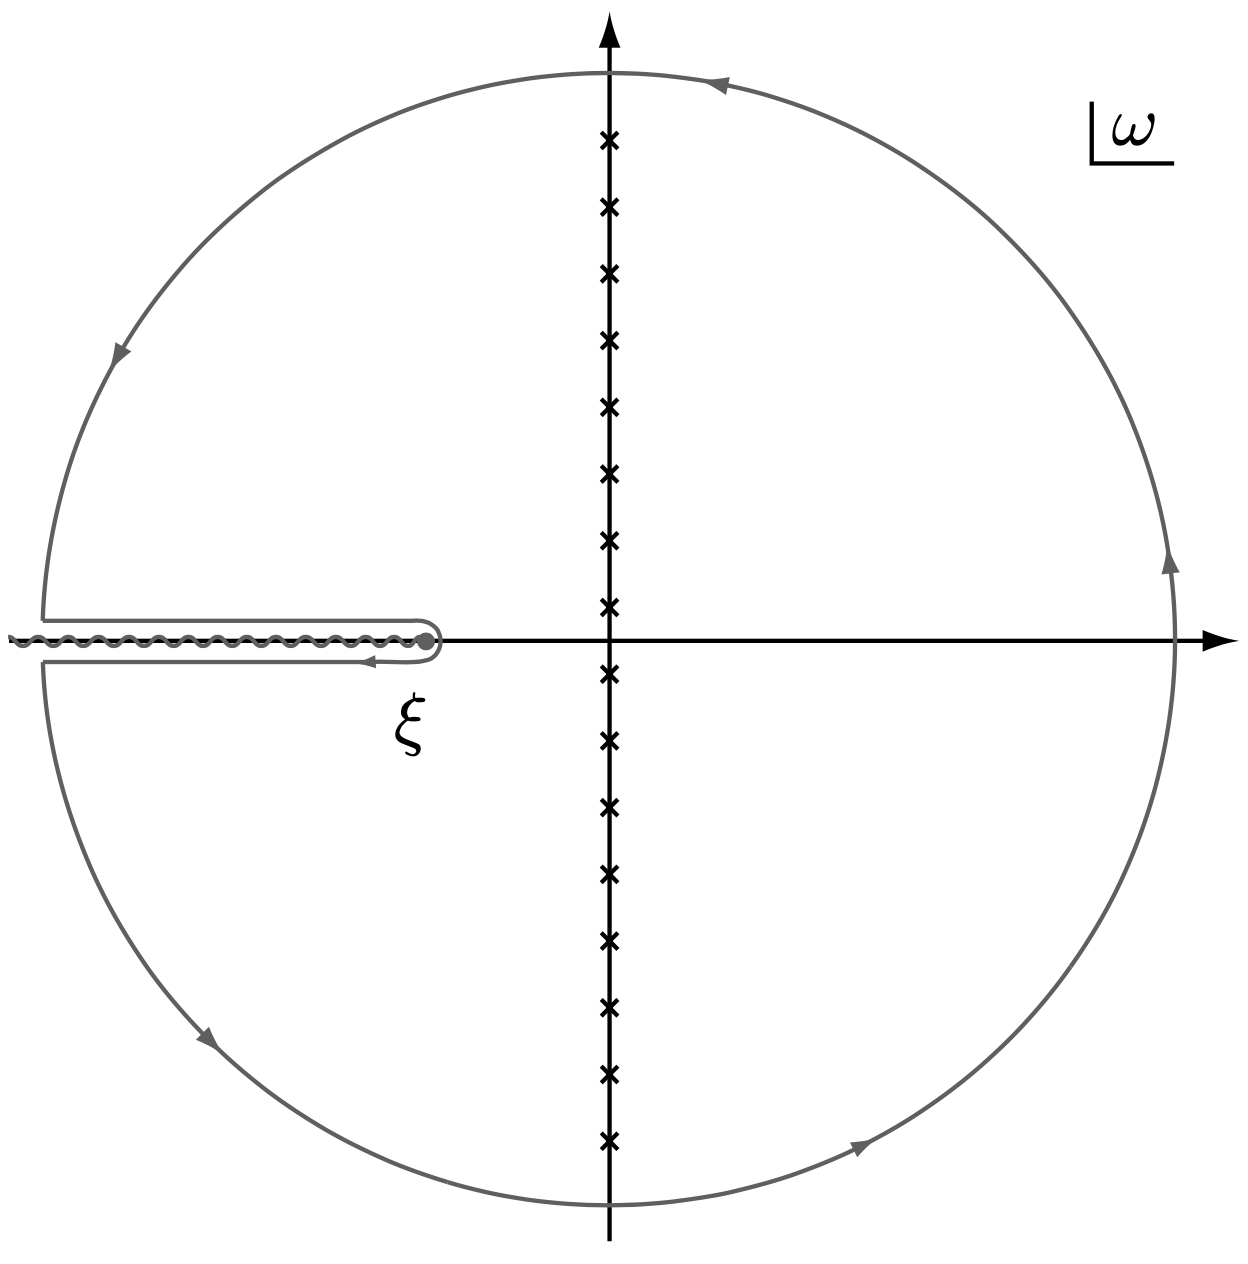
\includegraphics[width=0.25\linewidth]{pics/FqSum.png}
\end{equation*}
The free energy is
\begin{equation}
\begin{aligned}
	F &= \frac{1}{2\pi i}\int_{-\infty}^\infty dx \rho(x)\ln\left(\frac{\xi-x-i\epsilon}{\xi-x+i\epsilon}\right) \\
	&= \frac{-\zeta}{2\pi i\beta} \int_{-\infty}^{\infty}dx \ln(1-\zeta e^{-\beta z})\left(\frac{1}{x+i\epsilon-\xi}-\frac{1}{x-i\epsilon-\xi}\right),
\end{aligned}
\end{equation}
where we integrate the expression by part, noticing that
\begin{equation}
	\frac{d}{dz} \frac{\zeta}{\beta} \ln(1-\zeta e^{-\beta z}) = \frac{1}{e^{\beta z}-\zeta} = \rho(z)
\end{equation}
Using the identity
\begin{equation*}
	\lim_{\epsilon\rightarrow 0^+} \frac{1}{x+i\epsilon} = -i\pi\delta(x) + \mathcal{P}\frac{1}{x},
\end{equation*}
the above expression can be simplified to
\begin{equation}
	F = \frac{\zeta}{\beta} \ln(1-\zeta e^{-\beta\zeta}).
\end{equation}


\section{Fermi Liquid Theory}
In this section, we are considering the system of weakly interacting Fermi gas.
To be specific, we consider the lattice Hamiltonian:
\begin{equation}\label{eq:FL-gen-ham}
	H = -\frac{1}{2}\sum_{\langle i,j \rangle} (c_i^\dagger c_{j} + c_{j}^\dagger c_i) + \mu\sum_i c_i^\dagger c_i + \sum_{i,j,k,l} u_{ijkl} c_i^\dagger c_j^\dagger c_k c_l.
\end{equation}
In the following, we investigate the effective field theory near the Fermi surface.
We discuss the RG flow of the couplings (mainly for two dimensional system).
Then we carry out the perturbative calculation for the correlation functions. 

\subsection{Effective Field Theory for Interacting Fermi Systems}
The low-energy manifold is an annulus of thickness $2 \Lambda$ symmetrically situated with respect to the Fermi circle $K=K_{\mathrm{F}}$.
The dispersion for the free lattice model is
\begin{equation}
	E(\bm K) = -\cos K_x - \cos K_y \simeq -2 + \frac{\bm K^2}{2}.
\end{equation}
For a given chemical potential $\mu$, the Fermi circle is $K_F = \sqrt{2m\mu}$, we can linearize the dispersion near the Fermi surface:
\begin{equation}
	E(\bm K) = \frac{\bm K^2-K_F^2}{2m} \simeq \frac{K_F}{m}k \equiv v_F k, \quad
	k\equiv |K|-K_F
\end{equation}
The partition function is:
\begin{equation}
	Z_0 = \sum_\theta \sum_{|k|<\Lambda}\int D\left[\bar\psi(k,\theta,\omega),\psi(k,\theta,\omega)\right] e^{-S_0},
\end{equation}
where the free field action is:\footnote{A factor of $K_{\mathrm{F}}$ has been absorbed in the field.}
\begin{equation}
	S_0 = \int \frac{d\theta}{2\pi} \int^\Lambda_{-\Lambda}\frac{dk}{2\pi} \int^\infty_{-\infty}\frac{d\omega}{2\pi} \bar\psi(k,\theta,\omega)(-i\omega+v_F k)\psi(k,\theta,\omega).
\end{equation}
Consider the quartic interaction
\begin{equation}
	\delta S_4 = \frac{1}{4}\int_{\bm K,\theta,\omega} \bar\psi(4)\bar\psi(3)\psi(2)\psi(1)u(4,3,2,1)
\end{equation}
where we eliminate one of the four sets of variables, say, the one numbered 4, by integrating them against the delta functions:
\begin{equation}
	\int_{K,\theta,\omega}
	=\prod_{i=1}^{3} \int_{0}^{2 \pi} \frac{d \theta_{i}}{2 \pi} \int_{-\Lambda}^{\Lambda} \frac{d k_{i}}{2 \pi} \int_{-\infty}^{\infty} \frac{d \omega_{i}}{2 \pi} \theta\left(\Lambda-\left|k_{4}\right|\right), \quad 
	k_4 = |\bm K_4|-K_F.
\end{equation}
The $\omega$ integral is easy: since all $\omega$'s are allowed, the condition $\omega_4=\omega_1+\omega_2-\omega_3$ is always satisfied for any choice of the first three frequencies. 
The same would be true for the momenta if all momenta were allowed. 
But they are not; they are required to lie within the annulus of thickness $2\Lambda$ around the Fermi circle. 
Consequently, if one freely chooses the first three momenta from the annulus, the fourth could have a length as large as $3K_F$. 
The role of $\delta(\Lambda-|k_4|)$ is to prevent exactly this.

\subsubsection*{Momentum Constraint}
Note that $k_4$ can be expressed as
\begin{equation}
	k_4 = |(K_F+k_1)\bm \Omega_1+(K_f+k_2)\bm \Omega_2-(K_F+k_3)\bm \Omega_3|-K_F.
\end{equation}
When doing RG towards the Fermi surface, the integral measure will not preserve the preserve the original form.
The situation is clearly is we use a smooth cutoff
\begin{equation}
	\theta(\Lambda-|k_4|) \rightarrow e^{-|k_4|/\Lambda},
\end{equation}
and define $\Delta\equiv \bm \Omega_1+\bm \Omega_2-\bm \Omega_3$, $k_4$ in this way behaves as
\begin{equation}
	k_4 = (|\Delta|-1)K_F + O(k).
\end{equation}
The integral then change to:
\begin{equation}
\begin{aligned}
	& \prod_{i=1}^{3} \int_{-\Lambda}^{\Lambda} \frac{d k_{i}}{2\pi} 
		\int \frac{d \theta_{i}}{2 \pi} \int \frac{d \omega_{i}}{2 \pi} 
		e^{-||\Delta|-1|\frac{K_F}{\Lambda}} u(k,\theta,\omega) 
		\bar\psi \bar\psi \psi \psi \\
	\overset{\mathrm{RG}}{\longrightarrow} & \prod_{1}^{3} \int_{-\Lambda}^{\Lambda}
		\frac{d k_{i}^{\prime}}{2 \pi} 
		\int \frac{d \theta_{i}}{2 \pi} 
		\int \frac{d \omega_{i}^{\prime}}{2 \pi} 
		e^{-|| \Delta|-1|\frac{sK_F}{\Lambda}} 
		u\left(\frac{k^{\prime}}{s} \frac{\omega^{\prime}}{s} \theta\right) 
		\bar\psi \bar\psi \psi \psi.
\end{aligned}
\end{equation}
We can then get the RG transformation of $u$ as
\begin{equation}
	u'(k',\theta,\omega') = e^{-||\Delta|-1|\frac{(s-1)K_F}{\Lambda}}u\left(\frac{k'}{s},\theta,\frac{\omega'}{s}\right).
\end{equation}
By Taylor expansion, we conclude that the only couplings that survive the RG transformation without any decay correspond to the cases in which $|\Delta|=1$, and without momentum dependence.

\begin{figure}[]
	\centering
	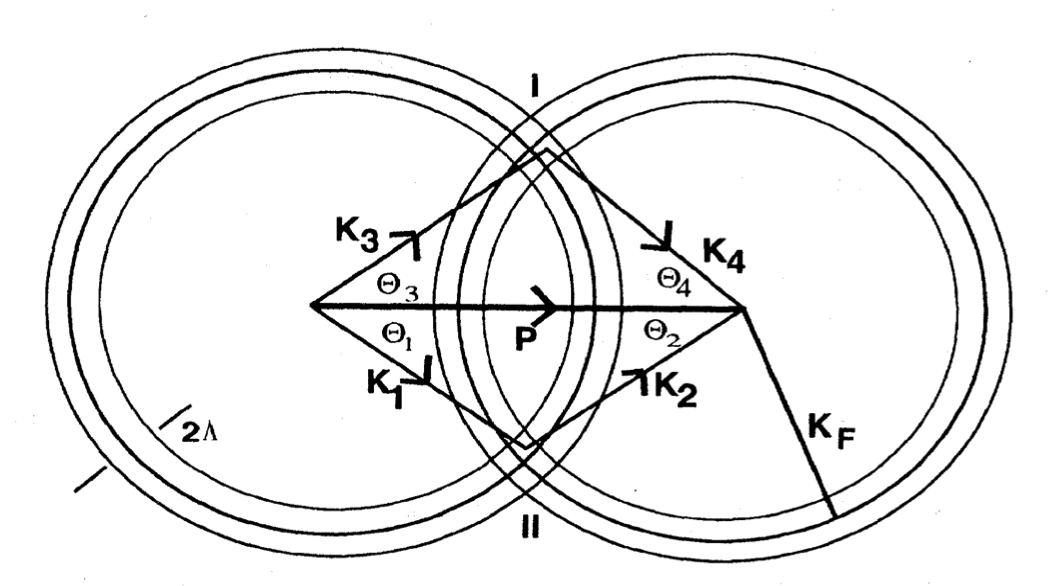
\includegraphics[width=0.5\linewidth]{pics/FL-kcons.png}
	\caption{The geometric construction for determining the allowed values of momenta. If $K_{1}$ and $K_{2}$ add up to $P$, then $K_{3}$ and $K_{4}$ are constrained as shown, if they are to add up to $P$ and lie within the cutoff. If the incoming momenta $K_{1}$ and $K_{2}$ are equal and opposite, the two shells coalesce and $K_{3}$ and $K_{4}$ are free to point in all directions, as long as they are equal and opposite.}
	\label{fig:FL-kcons}
\end{figure}

This equation has only three solutions (see also Fig.~\ref{fig:FL-kcons}):
\begin{equation}
\begin{aligned}
	&\text{Case I:} \quad \bm \Omega_1 = \bm \Omega_3, \\
	&\text{Case II:} \quad \bm \Omega_2 = \bm \Omega_3, \\
	&\text{Case III:} \quad \bm \Omega_1 = -\bm \Omega_2.
\end{aligned}
\end{equation}
Because of the rotational symmetry, the marginal vertex functions are determined solely by two functions:
\begin{eqnarray}
	u[\theta_1,\theta_2,\theta_1,\theta_2] &\equiv& F(\theta_1,\theta_2) = F(\theta_1-\theta_2), \\
	u[\theta_1,\theta_2,\theta_2,\theta_1] &=& -F(\theta_1-\theta_2), \\
	u[\theta_1,-\theta_1,\theta_3,-\theta_3] &\equiv& V(\theta_1,\theta_3) = V(\theta_1-\theta_3).
\end{eqnarray}
Note that the manifestation of the Pauli principle on $F$ and $V$ is somewhat subtle: $F$ will not be antisymmetric under $1 \leftrightarrow 2$ since, according to the way it is defined above, we cannot exchange 1 and 2 without exchanging 3 and 4 at the same time. 
On the other hand, since 3 and 4 can be exchanged without touching 1 and 2 in the definition of $V$, $V$ must go to $-V$ when $1 \leftrightarrow 3$.

\subsection{One-loop RG for 2D System}
We first consider the loop correction to the chemical potential:
\begin{equation}
\begin{aligned}
	\mu^{(2)}(k,\theta,\omega) 
	&= \int_{d\Lambda}\frac{dK'}{2\pi} \int \frac{d\omega'}{2\pi} \int \frac{d\theta'}{2\pi} \frac{F(\theta-\theta')}{i\omega-v_F k'} \\
	&= \int_{-\Lambda}^{-\Lambda+\Lambda dt}\frac{dK'}{2\pi} \int \frac{d\theta'}{2\pi} F(\theta-\theta') \\
	&= \frac{\Lambda}{2\pi} \left[\int\frac{d\phi}{2\pi} F(\phi)\right] dt.
\end{aligned}
\end{equation}
For the vertex correction, again we should consider three channels corresponding to the diagrams:
\begin{equation}
	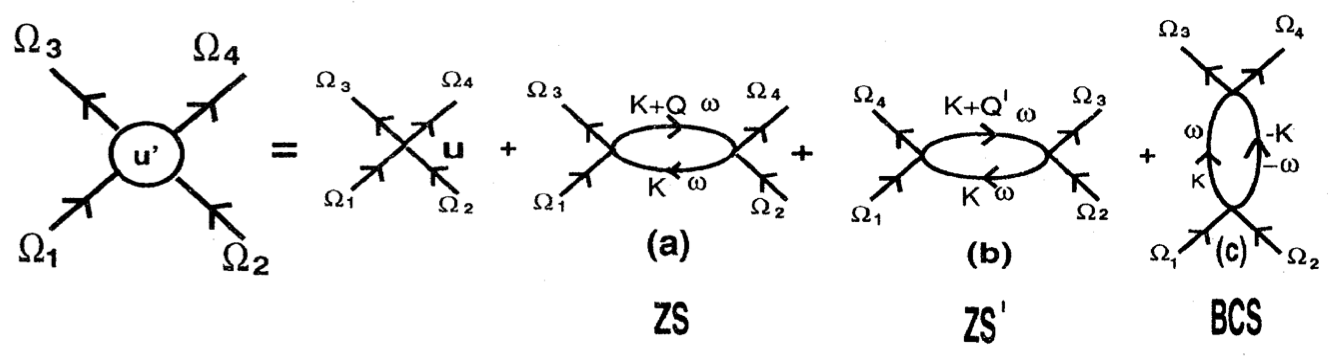
\includegraphics[align=c, width=0.7\linewidth]{pics/FL-4.png}
\end{equation}
First we consider the correction to the $F(\theta)$.
The contribution from the ZS channel (the momentum transfer $Q \simeq 0$) is
\begin{equation}
	F^{(2)}_{\mathrm{ZS}}(\theta_1-\theta_2) = \int_{d\Lambda}\frac{dk}{2\pi}\int \frac{d\omega}{2\pi} \int \frac{d\theta}{2\pi} \frac{F(\theta_1-\theta)F(\theta-\theta_2)}{(i\omega-v_F k)^2}.
\end{equation}
Since two poles of the integrant lie at the same half plane, we can alway choose to close the loop integral along the other half, and thus getting zero contribution.

\begin{figure}[]
	\centering
	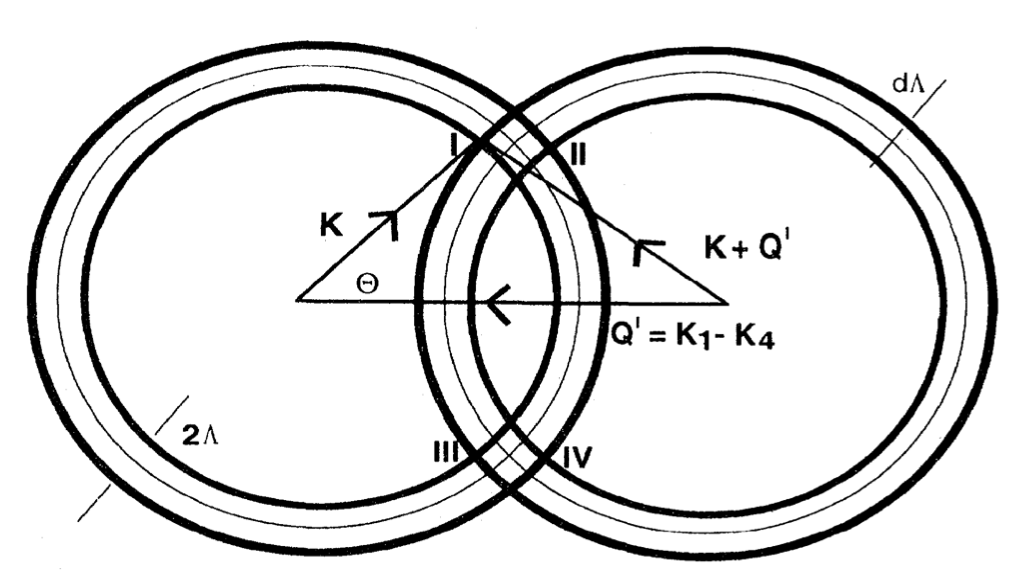
\includegraphics[width=0.4\linewidth]{pics/FL-kshell.png}
	\caption{Construction for determining the allowed values of loop momenta in ZS'. The requirement that the loop momenta come from the shell and differ by $Q'$ forces them to lie in one of the eight intersection regions of width $d\Lambda^2$.}
	\label{fig:FL-kshell}
\end{figure}

For the ZS' channels, the momentum conservation condition (see Fig.~\ref{fig:FL-kshell}) restrict the phase space to be of order $d\Lambda^2$, and thus has no relevant contribution to $F(\theta)$.
Finally, for the same kinematical reason, the BCS diagram does not renormalize $F(\theta)$ at one loop.
Consider Fig.~\ref{fig:FL-kcons}, with $K_3$ and $K_4$ replaced by the two momenta in the BCS loop, $K$ and $P-K$.
In each annulus we keep just two shells of thickness $d\Lambda$ at the cutoff corresponding to the modes to be eliminated. 
The requirement that $K$ and $P-K$ lie in these shells and also add up to $P$ forces them into intersection regions of order $d\Lambda^2$. 
This means the diagram is just as ineffective as the ZS' diagram in causing a flow. 
Thus any $F$ is a fixed point to this order.

Now we consider the correction to the $V(\theta)$ function.
We choose the external momenta equal and opposite and on the Fermi surface. 
The ZS and ZS' diagrams do not contribute to any marginal flow for the same reason that BCS and ZS' did not contribute to the flow of $F(\theta)$.
But the BCS diagram produces a flow:
\begin{equation}
\begin{aligned}
	V^{(2)}_{\mathrm{BCS}}(\theta_1-\theta_3) 
	&= -\frac{1}{2}\int_{d\Lambda}\frac{dk}{2\pi}\int\frac{d\omega}{2\pi}\int\frac{d\theta}{2\pi} 
		\frac{V(\theta_1-\theta)V(\theta-\theta_3)}{(i\omega-v_F k)(-i\omega-v_F k)} \\
	&= -\frac{dt}{4\pi v_F}\int \frac{d\theta}{2\pi}V(\theta_1-\theta)V(\theta-\theta_3).
\end{aligned}
\end{equation} 
We can simplify the picture by going to angular momentum eigenfunctions,
\begin{equation}
	V(\theta) = \sum_l e^{il\theta} V_l,
\end{equation}
which gives the RG flow as
\begin{equation}
	\frac{dV_l}{dt} = -\frac{V_l^2}{4\pi v_F}.
\end{equation}
The solution to the RG flow is:
\begin{equation}
	V_l(t) = \frac{V_l(0)}{1+\frac{V_l(0)}{4\pi v_F}t}.
\end{equation}
What these equations tell us is that if the potential in angular momentum channel $l$ is repulsive, it will get renormalized (logarithmically) down to zero, while if it is attractive, it will run off to large negative values signaling the BCS instability. 
This is the reason the $V$'s are excluded in Landau theory, which assumes we have no phase transitions.\footnote{Remember that the sign of any given $V_l$ is not necessarily equal to that of the microscopic interaction. Kohn and Luttinger have shown (PRL, 15, 524 (1965)) that some of them will be always negative. Thus, the BCS instability is inevitable, though possibly at absurdly low temperatures or absurdly high angular momentum $l$.}




\chapter{Luttinger Liquid}

\begin{figure}
	\centering
	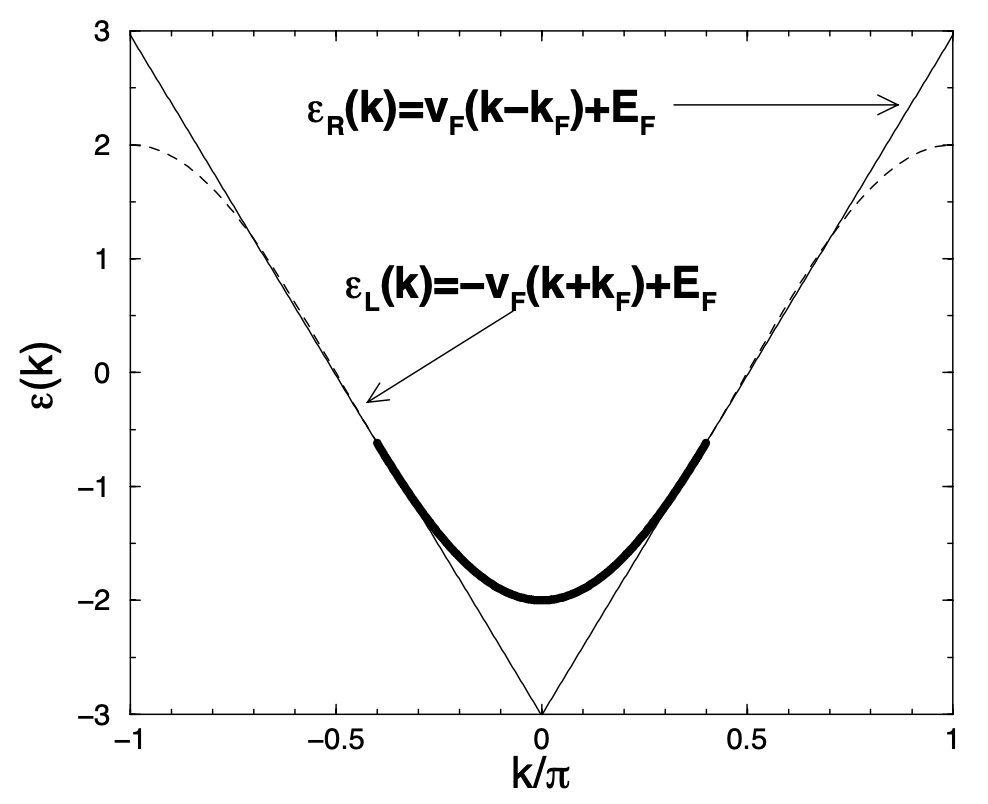
\includegraphics[width=0.4\linewidth]{pics/LL-linearize.png}
	\caption{Linearized Model.}
	\label{fig:bs-linearize}
\end{figure}

In this section, we discuss the one-dimensional interacting Fermi system, described by the Hamiltonian
\begin{equation}
	H = -\frac{1}{2}\sum_{i} (c_i^\dagger c_{i+1} + c_{i+1}^\dagger c_i) + \mu\sum_i c_i^\dagger c_i + \sum_{i,j,k,l} u_{ijkl} c_i^\dagger c_j^\dagger c_k c_l.
\end{equation}
The dispersion for the free theory is 
\begin{equation}
	\varepsilon(k) = -\cos k, \quad 
	v_F = \partial_k \varepsilon(k)|_{k=k_F} = \sin k_F.
\end{equation}
Near the Fermi surface with momentum $k_F$, the spectrum can be approximately linearized (as shown in Fig.~\ref{fig:bs-linearize}), with the left and right moving fermion modes:
\begin{equation}
	\varepsilon_{R/L}(k) = \begin{cases}
		v_F (k - k_F) & r=R \\
		-v_F (k + k_F) & r=L
	\end{cases}.
\end{equation}
The fermi momentum is (assume $N_L=N_R$)
\begin{equation}
	k_F = \frac{\pi N}{2L}.
\end{equation}
The state while all fermion modes filled below the Fermi surface and all modes empty above the Fermi surface is defined as the vacuum state $|0\rangle_0$.



\section{Field Theory for Luttinger Liquid}

In this section, we gives a field theoretical analysis of the interacting fermion system in 1D.
For the notational simplicity, we shift the momentum so that
\begin{equation}
	k \rightarrow k' = \begin{cases}
		k - k_F & r=R \\
		-k - k_F & r=L
	\end{cases}.
\end{equation}
The dispersion is then $\varepsilon_r(k) = v_F k$.
In this way, two Fermi points are brought to the origin, the left and right moving branches have the same dispersion.
The integral over momentum shell for both species of fermion can then be denoted by
\begin{equation}
	\int^\Lambda \frac{dK}{2\pi} \equiv \int_{-\Lambda}^\Lambda \frac{dk_L}{2\pi} + \int_{-\Lambda}^\Lambda \frac{dk_R}{2\pi}.
\end{equation}



\subsection{Effective Field Theory}

The effective field theory for the free field is
\begin{equation}
	Z_0 = \prod_{r=L/R}\int D\left[\bar\psi_r(k,\omega),\psi_r(k,\omega)\right] e^{-S_0},
\end{equation}
where the free field action is
\begin{equation}
	S_0 = \sum_{r=L/R} \int^\Lambda_{-\Lambda} \frac{dk}{2\pi} \int^\infty_{-\infty} \frac{d\omega}{2\pi} 
	\bar\psi_r(k,\omega)[-i\omega + v_F k]\psi_r(k,\omega),
\end{equation}
which gives the free field propagator:
\begin{equation}
	G_r(k,\omega) = -\langle \psi_r(k,\omega)\bar\psi_r(k,\omega)\rangle 
	= \frac{1}{i\omega - v_F k}.
\end{equation}
We then consider the rescaling of the cut-off $\Lambda \rightarrow \Lambda/s$. 
To make the free action scale invariant, we define the rescaled variables:
\begin{equation}
	k' = sk, \quad \omega' = s\omega, \quad 
	\psi'_r(k',\omega') = s^{-3/2}\psi_r(k,\omega).
\end{equation}
Then we consider the perturbation from quadratic and quartic terms:
\begin{equation}
\begin{aligned}
	\delta S_2 &= \sum_{r=L/R} \int^\Lambda_{-\Lambda}\frac{dk}{2\pi}\int^\infty_{-\infty} \frac{d\omega}{2\pi} 
	\mu(k,\omega) \bar\psi_r(k,\omega) \psi_r(k,\omega), \\
	\delta S_4 &= \frac{1}{2!2!} \int^\Lambda_{K,\omega} 
	u(4,3,2,1)\bar\psi(4)\bar\psi(3)\psi(2)\psi(1),
\end{aligned}
\end{equation}
where we have suppressed the momentum labels: 
\begin{equation}
	\psi(i) = \psi_{r_i}(k_i,\omega_i), \quad
	u(4,3,2,1) = u(K_4,\omega_4;K_3,\omega_3;K_2,\omega_2;K_1,\omega_1),
\end{equation}
and the integral is defined as:\footnote{The symbol $\bar\delta$ enforces momentum conservation mod $2\pi$, as is appropriate to any lattice problem. A process where lattice momentum is violated in multiples of $2\pi$ is called an \textit{umklapp process}.}
\begin{equation}
\begin{aligned}
	\int_{K \omega}^{\Lambda}
	=& \ \int^\Lambda \frac{d K_1 \cdots d K_4}{(2 \pi)^{4}} \int_{-\infty}^{\infty} \frac{d \omega_{1} \cdots d \omega_{4}}{(2 \pi)^{4}} \times 2 \pi \delta\left(\omega_{1}+\omega_{2}-\omega_{3}-\omega_{4}\right) \\
	&\ \times 2 \pi \bar{\delta}(K_1+K_2-K_3-K_4).
\end{aligned}
\end{equation}
Since this action separates into slow and fast pieces, the effect of mode elimination is simply to reduce $\Lambda$ to $\Lambda/s$ in the integral above. Rescaling moments and fields, we find that
\begin{equation}
	\mu'(k',\omega') = s\cdot\mu\left(\frac{k'}{s}, \frac{\omega}{s}\right).
\end{equation}
Expand $\mu$ in series:
\begin{equation}
	\mu(k, \omega)=\mu_{00}+\mu_{10} k+\mu_{01} i \omega+\cdots+\mu_{n m} k^{n}(i \omega)^{m}+\cdots,
\end{equation}
and compare both sides. The constant piece is a relevant perturbation.
This relevant flow reflects the readjustment of the Fermi sea to a change in chemical potential. 
The correct way to deal with this term is to include it in the free-field action by filling the Fermi sea to a point that takes $\mu_{00}$ into account. 
The next two terms are marginal and modify terms that are already present in the action.

We now turn on the quartic interaction, the dimensional analysis gives the transformation of $u$:
\begin{equation}
	u'_{i_4,i_3,i_2,i_1}(k'_i,\omega'_i) = u_{i_4,i_3,i_2,i_1}\left(\frac{k'_i}{s},\frac{\omega'_i}{s}\right).
\end{equation}
If we expand $u$ in a Taylor series in its arguments and compare coefficients, we find that the constant term u0 is marginal and the higher coefficients are irrelevant. 
Thus, $u$ depends only on its discrete labels and we can limit the problem to just a few coupling constants instead of the coupling function we started with. 
Furthermore, all reduce to just one coupling constant:
\begin{equation}
	u_0 = u_{LRLR} = u_{RLRL} = -u_{RLLR} = -u_{LRRL} \equiv u.
\end{equation}
Other couplings corresponding to the ($LL \rightarrow RR$) process are wiped out by the Pauli principle since they have no momentum dependence and cannot have the desired antisymmetry.

\subsection{RG at One-loop Level}

Consider the infinitesimal rescale $s=e^{dt}$. 
The one-loop contribution to the quadratic term is\footnote{We include an infinitesimal $e^{i\omega\eta}$ to ensure convergence as we do the integral over $\omega$ by closing the upper half-plane.}
\begin{equation}
	\mu^{(2)}_{LL} = 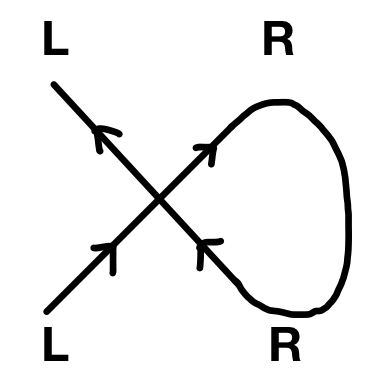
\includegraphics[align=c, width=0.125\linewidth]{pics/LL-1.png}
	= -u \int_{d\Lambda} \frac{dk}{2\pi}\int^\infty_{-\infty}\frac{d\omega}{2\pi}\frac{e^{i\omega \eta}}{i\omega - v_F k},
\end{equation}
where the integral on the momentum shell is
\begin{equation}
	\int_{d\Lambda}\frac{dk}{2\pi} = \int_{-\Lambda}^{-\Lambda(1-dt)} \frac{dk}{2\pi} + \int_{\Lambda(1-dt)}^{\Lambda} \frac{dk}{2\pi}.
\end{equation}
The result gives:
\begin{equation*}
	\mu^{(2)}_{LL}
	= -\frac{u\Lambda}{2 \pi}dt
\end{equation*}
By the symmetry $L \leftrightarrow R$, we know $\mu^{(2)}_{LL}=\mu^{(2)}_{RR}=\mu^{(2)}$, so the RG flow is
\begin{equation}
	\frac{d}{dt}\left[s\cdot\left(\mu+\mu^{(2)}\right)\right] = \mu - \frac{u\Lambda}{2\pi}.
\end{equation}
The one-loop correction to the quartic term ($u_{LRRL}=-u$) have two contributions.
One is called ZS' (zero sound) channel:\footnote{There is actually another zero sound channel ZS, but which has no contribution to the vertex because the diagram contains the vertex of the ($LL \rightarrow RR$) process, which has no relevant contribution the the vertex.}
\begin{equation}
\begin{aligned}
	u^{(2)}_{\mathrm{ZS'}} 
	&= 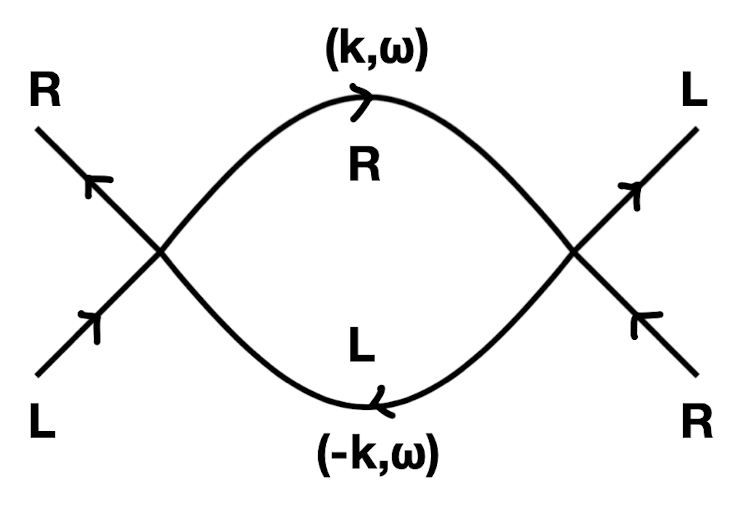
\includegraphics[align=c, width=0.2\linewidth]{pics/LL-2.png} \\
	&= -u^2 \int^\infty_{-\infty}\int_{\Lambda/s<|k|<\Lambda} \frac{d\omega dk}{(2\pi)^2} \frac{e^{i\omega\eta}}{(i\omega+v_F k)(i\omega-v_F k)} \\
	&= u^2\int_{\Lambda/s<|k|<\Lambda} \frac{dk}{2\pi} \frac{1}{2|k|} \\
	&= \frac{u^2}{2\pi}\frac{d\Lambda}{\Lambda}.
\end{aligned}
\end{equation}
The sign is obtained from contracting the Fermion field monomial:
\begin{equation*}
	\wick{
        \c1 {\bar\psi}_L \bar\psi_R \psi_L \c2 \psi_R
        \bar\psi_L \c2 {\bar\psi}_R \c1 {\psi}_L \psi_R
	} = -G_L G_R \bar\psi_R \psi_L \bar\psi_L \psi_R
	= -G_L G_R \bar\psi_L \bar\psi_R \psi_L \psi_R.
\end{equation*}
The other is called the BCS channel:\footnote{The $1/2$ factor comes from the symmetry factor of the diagram.}
\begin{equation}
	u^{(2)}_{\mathrm{BCS}} 
	= 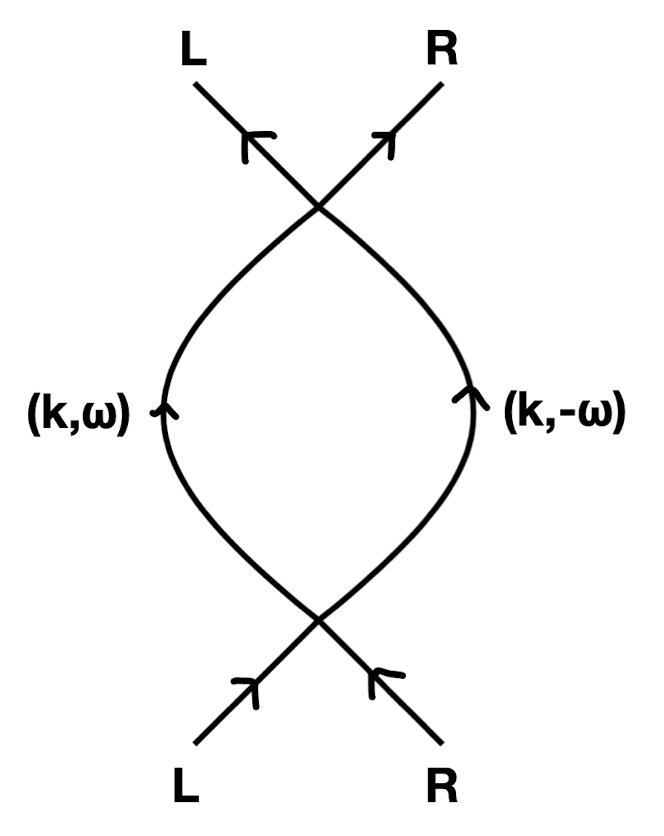
\includegraphics[align=c, width=0.15\linewidth]{pics/LL-3.png} 
	= -\frac{u^2}{2} \sum_{r=L/R}\int^\infty_{-\infty}\int_{d\Lambda} \frac{d\omega dk_i}{(2\pi)^2} \frac{e^{i\omega\eta}}{(i\omega-v_F k)(-i\omega-v_F k)}.
\end{equation}
The sign is obtained from the contraction:
\begin{equation*}
	\wick{
        \bar\psi_L \bar\psi_R \c1 \psi_L \c2 \psi_R
        \c1 {\bar\psi}_L \c2 {\bar\psi}_R \psi_L \psi_R
	} = -G_L G_R \bar\psi_L \bar\psi_R \psi_L \psi_R.
\end{equation*}
Note that we will obtained a factor of 2 since in this channel, the intermedia propagator can be left mover or right mover.
We see that two contributions cancel out:
\begin{equation}
	u^{(2)}_{\mathrm{ZS'}} + u^{(2)}_{\mathrm{BCS}} = 0.
\end{equation}
Together, the RG flow to the one-loop level is
\begin{equation}
	\frac{d\mu}{dt} = \mu - \frac{u\Lambda}{2\pi}, \quad
	\frac{du}{dt} = 0.
\end{equation}
The fixed point solution to the RG flow is:
\begin{equation}
	\mu^* = \frac{u^*\Lambda}{2\pi},
\end{equation}
where the fixed-point value of $u^*$ is arbitrary. 
The vanishing beta function predict that at least for small interaction, the system does not immediately develop a CDW order.
However, as the vertex function is marginal in the RG analysis, the fix points become a fixed line.
When the coupling $u$ is nonzero, the analysis for the Gaussian fix point becomes untrustworthy.
Actually when $u$ is getting sufficiently large, the umklapp process becomes relevant and the system flows to CDW phase.
A more systematic analysis requires the bosonization techniques. 


\section{Bosonization}

\subsection{Bosonic Hilbert Space}

In this section, we map the 1D interacting fermion system to a bosonic one.
The low energy excitations are particle-hole modes:
\begin{equation}
	\rho_{k}^\dagger = \sum_{q} c_{q+k}^\dagger c_{q}, \quad
	\rho_{k} = \sum_{q} c_{q}^\dagger c_{q+k} = \rho_{-k}^\dagger.
\end{equation}

To simplify the discussion, here we consider only a single branch of Fermion, as depicted in Fig.~\ref{fig:bs-hilbert}. The generalization to multiple branches is trivial since the dispersion is the same.

\begin{figure}
	\centering
	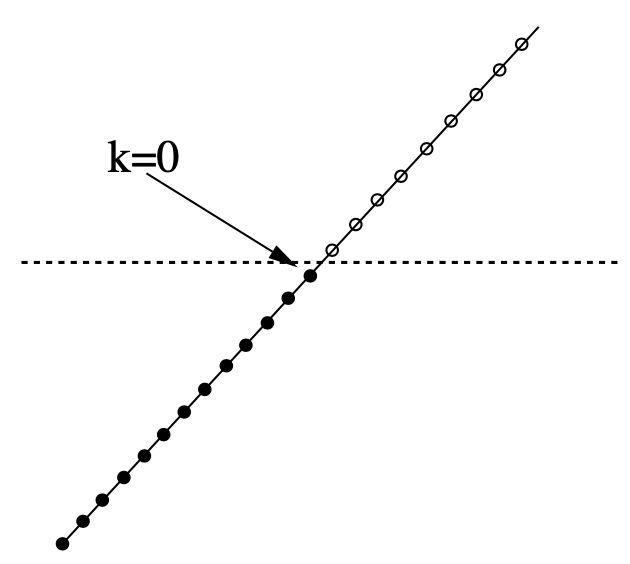
\includegraphics[width=0.25\linewidth]{pics/LL-hilbert.png}
	\caption{The vacuum state $|0\rangle_0$ of a single fermion branch.}
	\label{fig:bs-hilbert}
\end{figure}

\subsubsection*{Commutation Relation}
The commutation relation between $\rho_k$ and $\rho_{k'}^\dagger$ is:\footnote{We use the identity $[AB,C] = A[B,C] + [A,C]B$ and $[A,BC]=\{A,B\}C - B\{A,C\}$.}
\begin{equation}
\begin{aligned}
	\left[\rho_{k}, \rho_{k'}^\dagger \right]
	&= \sum_{q_1, q_2} \left[c_{q_1}^\dagger c_{q_1+k}, c_{q_2+k'}^\dagger c_{q_2}\right] \\
	&= \sum_{q_1, q_2} \left\{c_{q_1}^\dagger \left[c_{q_1+k}, c_{q_2+k'}^\dagger c_{q_2}\right] +\left[c_{q_1}^\dagger, c_{q_2+k'}^\dagger c_{q_2}\right] c_{q_1+k}\right\} \\
	&= \sum_{q_1, q_2} \left\{ \delta_{q_1+k,q_2+k'} c_{q_1}^\dagger c_{q_2} -
		\delta_{q_1,q_2} c_{q_2+k'}^\dagger c_{q_1+k} \right\} \\
	&= \sum_{q}\left[c^\dagger_{q+k'-k} c_{q}-c^\dagger_{q+k'} c_{q+k}\right].
\end{aligned}
\end{equation}
For $k \ne k'$, it is clear that $[\rho_{k},\rho_{k'}^\dagger]=0$.
However, when $k = k'$, we should be careful about the subtraction, since it evolve two infinities of which the subtraction is ill-defined.

Here we deal with the infinity with the lattice regularization, i.e., we think of the linearized theory as the low-energy approximation of a lattice mode, where the dispersion form a single energy band.
The left/right movers are actually in a single band but with positive/negative momentum.
Consider for example the density operator for the right mover, the commutator of the right moving density operator is then
\begin{equation}
	\left[\rho_{k,r}, \rho_{k,r}^\dagger \right] = \sum_{0<q<\pi} [n_{q,r}-n_{k+q,r}].
\end{equation}

\begin{figure}
	\centering
	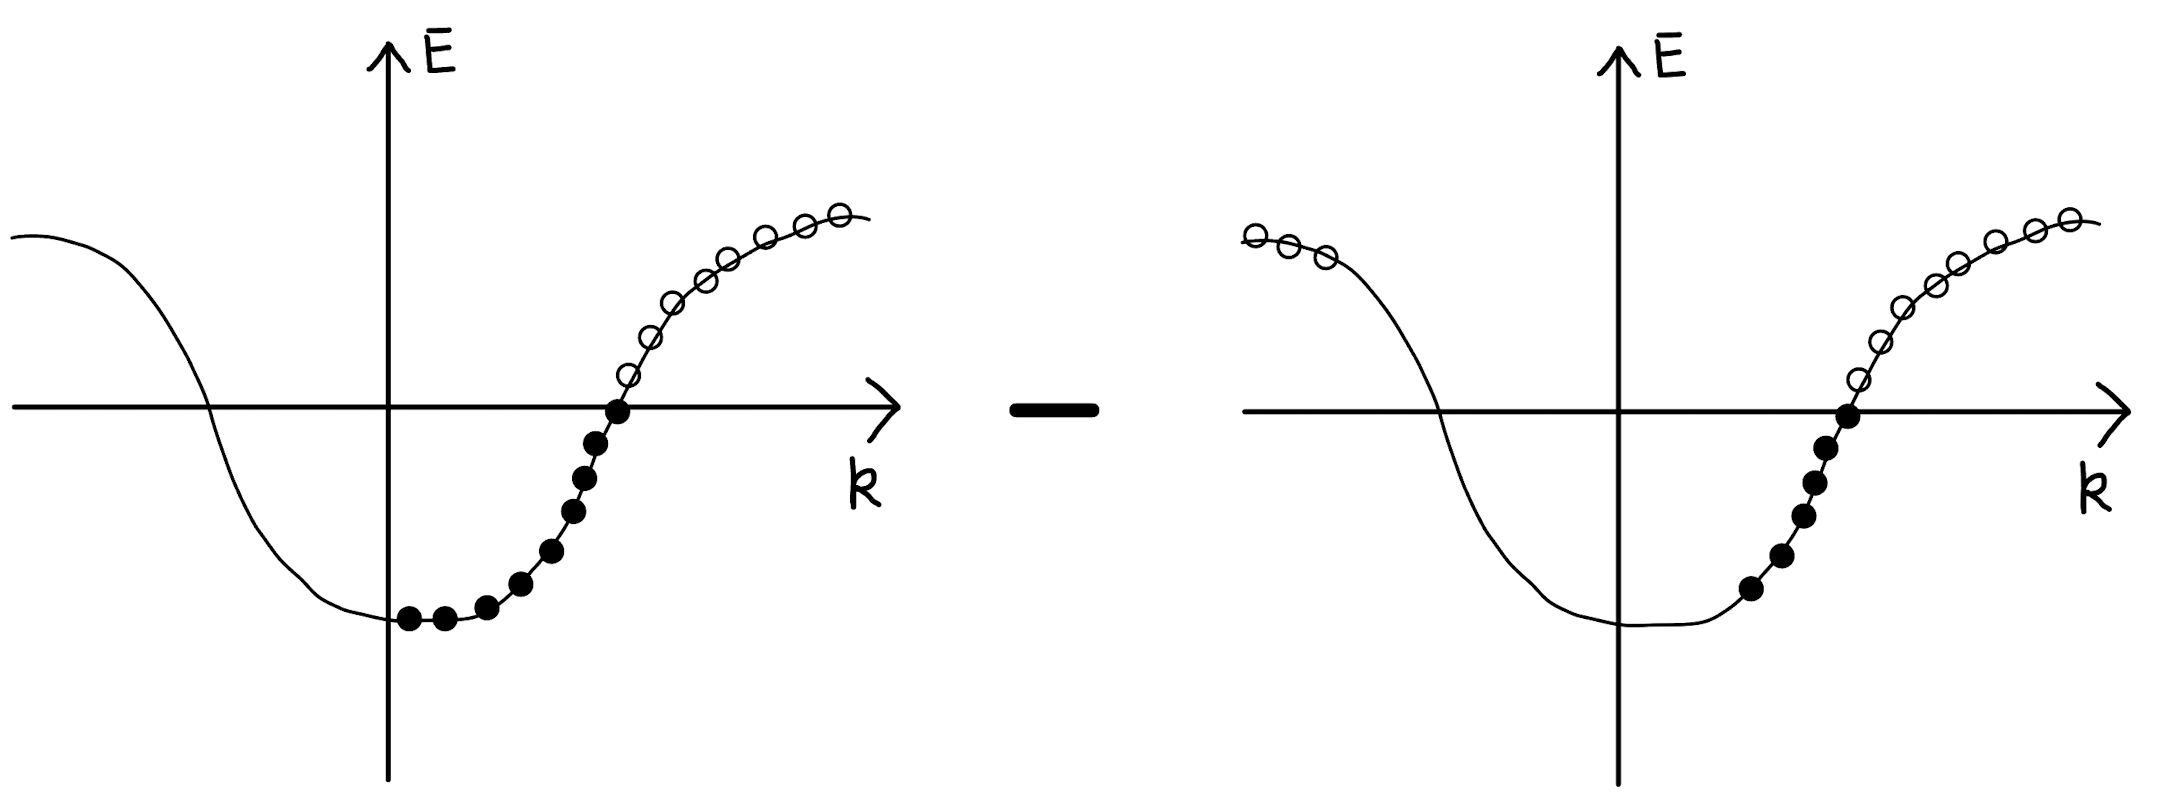
\includegraphics[width=0.5\linewidth]{pics/LL-k-shift}
	\caption{Shift of the right-moving modes.}
	\label{fig:bs-k-shift}
\end{figure}

Consider for example the case where $r=R,k>0$, as shown in Fig.~\ref{fig:bs-k-shift}.
The subtraction result in a sum of low-lying right-mover number operator minus a sum of high-energy left-mover number operator, which behaves like a constant in the low energy regime. 
The above analysis gives the commutation relation:
\begin{equation}
	\left[\rho_{k,r}, \rho_{kr}^\dagger \right] \simeq \frac{qL}{2\pi} \equiv n_q.
\end{equation}

Another way to deal with the infinity is by the normal-order expression:
\begin{equation}
	O = {:\mathrel{O}:} + \langle 0|O|0\rangle.
\end{equation}
For $k\ne k'$, since $\langle 0|c_k^\dagger c_k|0\rangle=0$, the normal ordering does not affect the result, while for the $k=k'$ case, the normal ordering takes care of the infinity of the particle number operator:
\begin{equation}
\begin{aligned}
	\sum_q [n_{q} - n_{q+k}]
	&= \sum_q \left[{:\mathrel{n_{q}}:} - {:\mathrel{n_{q+k}}:} 
		+ \langle0|n_{q}|0\rangle -\langle0|n_{q+k}|0\rangle \right] \\
	&= \sum_q [\langle0|n_{q}|0\rangle -\langle0|n_{q+k}|0\rangle].
\end{aligned}
\end{equation}
The final result gives the same result as the above discussions.

\subsubsection*{Particle-hole Excitation}
We denote the ground state with $N$ fermions as $|N\rangle_0$, which satisfies:
\begin{equation}
	\rho_{p>0}|N\rangle_0 = \rho^\dagger_{p<0}|N\rangle_0 = 0.
\end{equation}
We can thus define a set of canonical bosonic modes:
\begin{equation}
	b_p^\dagger = i\frac{\rho^\dagger_p}{\sqrt{n_p}}, \quad 
	b_p = -i\frac{\rho_p}{\sqrt{n_p}}, \quad [b_q,b_{q'}^\dagger] = \delta_{qq'}.
\end{equation}
We will assume $p>0$, and the $\pm i$ factor is a convention chosen for the future convenience.

Now we discuss the construction of the Hilbert space using the bosonic modes.
The $N$-particle sector is spanned by the states generated by applying $b_q^\dagger$'s to the ground state $|N\rangle_0$.
A general $N$-particle state has the form:
\begin{equation}
	|N\rangle = f(\{b_q^\dagger\})|N\rangle_0.
\end{equation}
Note that the bosonic mode $b_q$ does not change the particle number:\footnote{The particle number operator is defined by the normal order expression $\hat{N} = \sum_k {:\mathrel{c_{k}^\dagger c_{k}}:}$.}
\begin{equation}
	\left[\hat N, b_q \right] = \left[\hat N, b_q^\dagger \right] = 0.
\end{equation}
In order to construct the full Fock space, we also need to include a particle-number-changing operator, the \textit{Klein factor} $\hat F$, that shifts the total number of fermion by one, and commutes with bosonic operator $b_q$:
\begin{equation}
	\left[\hat F, b_q \right] = \left[\hat F, b_q^\dagger \right] = 0, \quad
	\left[\hat F, \hat N \right] = \hat F, \quad 
	\left[\hat F^\dagger, \hat N \right] = -\hat F^\dagger.
\end{equation}
For system with different fermion species (labeled by $\eta$), the set of operator
\begin{equation*}
	\{b_{q,\eta}, b_{q,\eta}^\dagger, \hat F_\eta, \hat N_\eta\}
\end{equation*}
form a complete operator basis for the Hilbert space within the low-energy regime.
However, note that the Klein factor also takes care of the fermionic statistics. 
That is, for the state denoted as
\begin{equation}
	|\{N_i\}\rangle = |N_1,N_2,\cdots,N_m\rangle
\end{equation}
The Klein factor $\hat F_\eta$ acting on the state will contribute an additional factor
\begin{equation}
	\hat F_\eta|\{N_i\}\rangle = \exp\left(i\pi\sum_{j=1}^{\eta-1}N_j\right)|N_1,\cdots,N_\eta-1,\cdots,N_m\rangle.
\end{equation}



\subsection{Bosonization of Fermion Field}
Now we try to express the fermion operator 
\begin{equation}
	\psi(x) = \frac{1}{\sqrt{L}} \sum_p e^{ipx} c_{p}
\end{equation}
by the bosonic operator set.
First we consider the commutation relation between the fermion field operator and bosonic mode:
\begin{equation}\label{eq:bs-comm-1}
\begin{aligned}
	\left[b_q,\psi(x)\right] &= \frac{1}{\sqrt L}\frac{i}{\sqrt{n_q}}\sum_{k}\sum_{p} e^{ipx} [c^\dagger_{k}c_{k+q,r'},c_{p}] \\
	&= -\frac{1}{\sqrt L} \frac{i}{\sqrt{n_q}} \sum_{p} e^{ipx} c_{p+q} 
	= -i\frac{1}{\sqrt{n_q}} e^{-iqx} \psi(x).
\end{aligned}
\end{equation}
Similarly,
\begin{equation}\label{eq:bs-comm-2}
	\left[b_q^\dagger,\psi(x)\right] = i\frac{e^{iqx}}{\sqrt{n_q}} \psi(x).
\end{equation}
For future convenience, we define a c-number factor:
\begin{equation}
	\alpha_q(x) \equiv \frac{1}{\sqrt{n_q}} e^{iqx},\quad
	[b_q^\dagger,\psi(x)] = i\alpha_q(x) \psi(x),\quad
	[b_q,\psi(x)] = -i \alpha^*_q(x) \psi(x).
\end{equation}
Since $b_q|N\rangle_0 = 0$, the commutation relation (\ref{eq:bs-comm-1}) leads to
\begin{equation}
	\left[b_{q}, \psi(x)\right]|N\rangle_{0} 
	=b_{q} \psi(x)|N\rangle_{0} 
	= -i\alpha_q^*(x) \psi(x)|N\rangle_{0}.
\end{equation}
Thus, $\psi(x)|N\rangle_0$ is an eigenstate of $b_q$, i.e., a coherent state:
\begin{equation}
	\psi(x)|N\rangle_0 
	= \Lambda(x) \hat F \exp\left[-i\sum_{q>0} \alpha_q^*(x) b_q^\dagger\right]|N\rangle_0
\end{equation}
where $\Lambda(x)$ is a c-number, which can be determined by
\begin{equation*}
	{}_{0}\langle N-1|\psi(x)| N\rangle_{0}=\Lambda(x)\ {}_{0}\langle N|\exp \left[-i\sum_{q>0} \alpha^*_q(x) b_{q}^{\dagger}\right]| N\rangle_{0} = \Lambda(x).
\end{equation*}
The left-hand side can be computed directly, the result is\footnote{Note that the Fermi point locates at $k_F=\frac{2\pi N}{L}$.}
\begin{equation}
	\Lambda(x) = \frac{1}{\sqrt L}\sum_k e^{ikx}\ {}_{0}\langle N-1| c_{k,r}|N\rangle_0 
	= \frac{1}{\sqrt L} e^{i\frac{2\pi N}{L}},
\end{equation}
In this way, we get
\begin{equation}
	\psi(x)|N\rangle_{0} = \frac{\hat F}{\sqrt{L}} e^{i \frac{2 \pi \hat{N} x}{L}} \exp \left[-i\sum_{q>0} \alpha^*_q(x) b_{q}^{\dagger}\right]|N\rangle_{0}
\end{equation}
The commutation relation (\ref{eq:bs-comm-2}) also leads to:\footnote{We denote $\alpha_q(x) \equiv e^{iqx}/\sqrt{n_q}$ to simplify the notation.}
\begin{equation*}
\begin{aligned}
	\psi(x) b_{q}^{\dagger} 
	&=\left[b_{q}^{\dagger}-i\alpha_{q}(x)\right] \psi(x) \\
	\Rightarrow \psi(x)\left(b_{q}^{\dagger}\right)^{n} 
	&=\left[b_{q}^{\dagger}-i\alpha_{q}(x)\right]^{n} \psi(x) \\
	\Rightarrow \psi(x) f\left[\left\{b_{q}^{\dagger}\right\}\right] 
	&=f\left[\left\{b_{q}^{\dagger}-i\alpha_{q}(x)\right\}\right] \psi(x).
\end{aligned}
\end{equation*}
Then, for a generic $N$-particle state:
\begin{equation}\label{eq:bs-temp1}
\begin{aligned}
	\psi(x)|N\rangle 
	&=f\left[\left\{b_{q}^{\dagger}-i\alpha_{q}(x)\right\}\right] \psi(x)|N\rangle_{0} \\
	&=f\left[\left\{b_{q}^{\dagger}-i\alpha_{q}(x)\right\}\right] \frac{\hat{F}}{\sqrt{L}} e^{i \frac{2 \pi \hat{N} x}{L}} \exp \left[-i\sum_{q>0} \alpha^*_{q}(x) b_{q}^{\dagger}\right]|N\rangle_{0} \\
	&=\frac{\hat{F}}{\sqrt{L}} e^{i \frac{2 \pi \hat{N} x}{L}} \exp \left[-i\sum_{q>0} \alpha^*_{q}(x) b_{q}^{\dagger}\right] f\left[\left\{b_{q}^{\dagger}-\alpha_{q}(x)\right\}\right]|N\rangle_{0}.
\end{aligned}
\end{equation}
Using the BCH formula
\begin{equation}
	e^A B e^{-A} = e^{[A,\cdot]} B = B + [A,B] + \frac{1}{2!}[A,[A,B]]+\cdots,
\end{equation}
we have the identity:
\begin{equation*}
\begin{aligned}
	\exp \left[-i\sum_{q>0} \alpha_{q}(x) b_{q}\right] b_{q}^{\dagger} \exp \left[i\sum_{q>0} \alpha_{q}(x) b_{q}\right] &=b_{q}^{\dagger}-i\alpha_{q}(x) \\
	\Rightarrow \exp \left[-i\sum_{q>0} \alpha_{q}(x) b_{q}\right] f\left[b_{q}^{\dagger}\right] \exp \left[i\sum_{q>0} \alpha_{q}(x) b_{q}\right] &=f\left[\left\{b_{q}^{\dagger}-i\alpha_{q}(x)\right\}\right].
\end{aligned}
\end{equation*}
Eq.~(\ref{eq:bs-temp1}) can be further simplified to:
\begin{equation*}
\begin{aligned}
	\psi(x)|N\rangle 
	=&\ \frac{\hat{F}}{\sqrt{L}} e^{i \frac{2 \pi \hat{N} x}{L}} e^{-i\sum_{q>0} \alpha^*_{q}(x) b_{q}^{\dagger}} e^{-i\sum_{q>0} \alpha_{q}(x) b_{q}} f\left[b_{q}^{\dagger}\right] e^{i\sum_{q>0} \alpha_{q}(x) b_{q}} |N\rangle_{0} \\
	=&\ \frac{\hat{F}}{\sqrt{L}} e^{i \frac{2 \pi \hat{N} x}{L}} \exp \left[-i\sum_{q>0} \alpha^*_{q}(x) b_{q}^{\dagger}\right] \exp \left[-i\sum_{q>0} \alpha_{q}(x) b_{q}\right]|N\rangle.
\end{aligned}
\end{equation*}
We thus express the Fermi field operator in bosonic operator:
\begin{equation}\label{eq:bs-fermi-field-1}
	\psi(x) = \frac{\hat{F}}{\sqrt{L}} e^{i \frac{2 \pi \hat{N} x}{L}} e^{-i\sqrt{2\pi}\varphi^\dagger(x)} e^{-i\sqrt{2\pi}\varphi(x)},
\end{equation}
where we have introduced a bosonic field:\footnote{The ``converging factor'' $e^{-a q / 2}$ is important in defining a proper bosonic theory in 1D. These equations should always be viewed as having $e^{-a q / 2}$ to ensure convergence at intermediate steps, but final results should be written taking $a \rightarrow 0^{+}$.}
\begin{equation}
	\varphi(x) = \frac{1}{\sqrt{2\pi}}\sum_{q>0} e^{-a q/2} a_{q}(x) b_{q}.
\end{equation}

\subsubsection*{Introduction of Bosonic Field}
Now we introducing the bosonic field:
\begin{equation}
	\phi(x) \equiv \varphi(x)+\varphi^{\dagger}(x)
	= \frac{1}{\sqrt{2\pi}} \sum_{q>0} \frac{e^{-a q/2}}{\sqrt{n_q}} \left[e^{i q x} b_{q}+e^{-i q x} b_{q}^{\dagger}\right].
\end{equation}
We can expressed the fermion field as:\footnote{We use the identity $e^A e^B = e^{A+B}e^{\frac{1}{2}[A,B]}$ if both $A$ and $B$ commutes with $[A,B]$.}
\begin{equation*}
	\psi(x) = \frac{\hat{F}}{\sqrt{L}} e^{i\frac{2\pi \hat N x}{L}} e^{-i\sqrt{2\pi}\phi(x)}
	e^{\pi[\varphi(x),\varphi^\dagger(x)]}.
\end{equation*}
The commutation relation between $\varphi$ and $\varphi^\dagger$ is
\begin{equation*}
	\left[\varphi(x),\varphi^\dagger(y)\right]
	= \frac{1}{L} \sum_q \frac{e^{iq(x-y+ia)}}{q} 
	= -\frac{1}{2\pi}\ln\left\{ 1-\exp\left[\frac{2\pi i}{L}(x-y+ia)\right]\right\}.
\end{equation*}
Set $x=y$, take limit $a\rightarrow 0^+$,
\begin{equation*}
	\exp\left\{\pi[\varphi(x),\varphi^\dagger(x)] \right\} = \lim_{a\rightarrow0^+} \left[1-\exp\left(-\frac{2\pi a}{L}\right)\right]^{-\frac{1}{2}}
	\rightarrow \sqrt{\frac{L}{2\pi a}}.
\end{equation*}
so we have
\begin{equation}\label{eq:bs-fermi-field}
	\psi(x) = \frac{\hat{F}}{\sqrt{2\pi a}}e^{i\frac{2\pi\hat N x}{L}}e^{-i\sqrt{2\pi}\phi(x)}.
\end{equation}
The divergent factor $1/\sqrt{2\pi a}$ appears because Eq.~(\ref{eq:bs-fermi-field}) is not normal-ordered.
We can check the result by normal-ordering the bilinear term $\psi^\dagger(x+a)\psi(x)$.
Insert Eq.~(\ref{eq:bs-fermi-field}) into the expression, we have:
\begin{equation}
	\psi^\dagger(x+a)\psi(x)
	\simeq \frac{e^{-i\frac{2\pi\hat N a}{L}}}{2\pi a}
	e^{i\sqrt{2\pi}\partial_x\phi(x)  a} 
	e^{\pi[\phi(x+ a),\phi(x)]}.
\end{equation}
The commutation relation is:
\begin{equation}
\begin{aligned}
	\left[\phi(x),\phi(y)\right] 
	&= -\frac{1}{2\pi}\ln \left\{\frac{1-\exp \left[\frac{2 \pi i}{L}(x-y+i  a)\right]}{1-\exp \left[-\frac{2 \pi i}{L}(x-y-i  a)\right]}\right\} \\
	&\stackrel{ a \rightarrow 0}{\longrightarrow} 
		\frac{i}{2} \operatorname{sgn}(x-y)-\frac{i}{L}(x-y).
\end{aligned}
\end{equation}
To the lowest order of $a/L$: 
\begin{equation}
	\psi^\dagger(x+a)\psi(x) \simeq \frac{i}{2\pi a} + \frac{\hat N+1}{L} - \frac{1}{\sqrt{2\pi}}\partial_x\phi(x).
\end{equation}
The normal ordering will delaminate all constant, including the divergent one:
\begin{equation}
	{:\mathrel{\psi^\dagger(x+a)\psi(x)}:}
	= \frac{\hat N}{L} - \frac{1}{\sqrt{2\pi}}\partial_x\phi(x).
\end{equation}
We will show in the following the above equation agrees with the bosonization of fermion bilinear $\psi^\dagger(x)\psi(x)$ term:
\begin{equation}
\begin{aligned}
	{:\mathrel{\psi^\dagger(x)\psi(x)}:}
	&= \frac{1}{L}\sum_{q} {:\mathrel{c_{q}^\dagger c_{q}}:} + \frac{1}{L}\sum_{q>0}[e^{-iqx}\rho^\dagger_{q}+e^{iqx}\rho_{q}] \\
	&= \frac{\hat N_r}{L} - \frac{1}{2\pi} \sum_{q>0} \frac{iq}{\sqrt{n_q}} \left[e^{iqx}b_{q} - e^{-iqx}b^\dagger_{q}\right].
\end{aligned}
\end{equation}
We then get:
\begin{equation}
	{:\mathrel{\psi^\dagger(x)\psi(x)}:}
	= \frac{\hat N}{L} - \frac{1}{\sqrt{2\pi}} \partial_x \phi(x).
\end{equation}

\subsubsection*{Effective Dirac Theory}
Now we consider the case where both the right-moving and left-moving fermion branches are involved.
Note that in the previous convention, the direction of momentum for left-mover is inverted, i.e., $\psi_L(k) = \tilde\psi(-k)$ for $k \sim -k_F$.
When take the Fourier transformation back to the coordinate space,
\begin{equation}
	\int_{-k_F-\Lambda}^{-k_F+\Lambda} \frac{dk}{2\pi} \tilde\psi(k) = \psi_L(-x),
\end{equation}
which would lead to $\psi(x) = \psi_R(x)+\psi_L(-x)$. 
To avoid such notational mess, we change the direction of the left-mover by defining $\psi_{\pm} = \psi_{R/L}(\pm x)$.
All the relations we have yet discussed are preserved, sometimes up to a change of coordinate: $x \rightarrow -x$, this amounts to 
\begin{equation}
	\psi_{\pm}(x) = \frac{1}{\sqrt{2\pi a}}e^{\pm i\frac{2\pi\hat N_{\pm} x}{L}}e^{-i\sqrt{2\pi}\phi_{\pm}(x)}.
\end{equation}
Note that from now on, we will constantly omit the Klein factor since for the calculation of correlation function, the Klein factors will alway cancel out finally.

Furthermore, we can shift the momentum $\pm k_F$ to the origin so that the free theory becomes a Dirac theory, with $N_{\pm}=0$.
The field expansion is now
\begin{equation}
\begin{aligned}
	\psi(x) &= e^{-ik_Fx} \int_{-\Lambda}^\Lambda \frac{dk}{2\pi} e^{ikx} \psi(-k_F+k)
	+ e^{ik_Fx} \int_{-\Lambda}^\Lambda \frac{dk}{2\pi} e^{ikx} \psi(k_F+k) \\
	&= e^{+ik_F x}\psi_+(x) + e^{-ik_F x}\psi_-(x).
\end{aligned}
\end{equation}

To better work with two fermion branches, we define a new set of bosonic fields:
\begin{equation}
	\phi(x) \equiv \frac{\phi_-(x) + \phi_+(x)}{\sqrt 2}, \quad
	\theta(x) \equiv \frac{\phi_-(x) - \phi_+(x)}{\sqrt 2}.
\end{equation}
Note that we can define a new set of canonical variables from these fields.
First consider the commutation relation
\begin{equation}
	[\phi(x),\theta(y)] \stackrel{ a \rightarrow 0}{\longrightarrow} 
		-\frac{i}{2} \operatorname{sgn}(x-y) + \frac{i}{L}(x-y)
\end{equation}
Define a new variable $\Pi(x) \equiv \partial_x\theta(x)$, the canonical commutation relation is:
\begin{equation}
	[\phi(x), \Pi(y)] = i \delta(x-y) - \frac{i}{L} \stackrel{L \rightarrow \infty}{\longrightarrow} i\delta(x-y).
\end{equation}
Note that the fermion fields can also be written as
\begin{equation}
	\psi_{\pm}(x) = \frac{1}{\sqrt{2\pi a}} \exp\left[-i\sqrt{\pi} \phi(x) \pm i\sqrt{\pi} \int^x_{-\infty} dy\ \Pi(y) \right].
\end{equation}


\subsection{Bosonization Dictionary}
\subsubsection{Bosonic Hamiltonian}
Now we go back to the Hamiltonian with linear dispersion (for single fermion branch):
\begin{equation}
	H_0 = v_F \sum_{k,r} k\ {:\mathrel{c_{k,r}^\dagger c_{k,r}}:} 
	= v_F \int dx\ {:\mathrel{\psi^\dagger(x)(-i\partial_x)\psi(x)}:}.
\end{equation}
Since $b_q^\dagger$ raise the energy of any eigenstate of $H_0$ by $q$ unit, we have the commutation relation:
\begin{equation}
	\left[H_0,b_{q,r}^\dagger\right] = q b_{q,r}^\dagger.
\end{equation}
The Hamiltonian satisfies such relation can only be the bosonic bilinear:
\begin{equation}
	H_0 = v_F \sum_{r}\sum_{q>0} q b_{q,r}^\dagger b_{q,r} + \frac{\pi v_F}{L} \sum_r \hat{N}_r(\hat{N}_r+1).
\end{equation}
The constant part comes from the fact that
\begin{equation}
	H_0|N\rangle_0 = \frac{2\pi v_F}{L} \frac{\sum_r\hat{N}_r(\hat{N}_r+1)}{2}|N\rangle_0, \quad
	b_{q,r}^\dagger b_{q,r} |N\rangle_0 = 0.
\end{equation}
Also, the bosonic operator can also be expressed as
\begin{equation}
	H_0 = \frac{v_F}{2} \int dx\ {:\mathrel{\left[\Pi^2 + (\partial_x \phi)^2\right]}:} + \frac{\pi v_F}{L}\sum_r \hat{N}_r(\hat{N}_r+1).
\end{equation}
Now consider the density-density interaction:
\begin{equation}
	\mathcal V_{\mathrm{int}} = u \int dx\ {:\mathrel{\psi^\dagger(x)\psi(x)}:}^2
\end{equation}
The fermion density operator is
\begin{equation}
\begin{aligned}
	\psi^\dagger(x)\psi(x) =&\ \psi_-^\dagger(x)\psi_-(x) + \psi_+^\dagger(x)\psi_+(x) + \\
	&\ e^{-2ik_F x} \psi_+^\dagger(x)\psi_-(x)+e^{2ik_F x}\psi_-^\dagger(x)\psi_+(x).
\end{aligned}
\end{equation}
The oscillation term is irrelevant unless the system is half-filled.
For the system away from half-filling, the bosonized interaction is also free:
\begin{equation}
	\mathcal V_\mathrm{int} = \frac{u}{2\pi}\sum_r \int dx\ (\partial_x\phi_r)^2.
\end{equation}

The half-filling case is more subtle.
In order to be more precise, we consider the lattice Hamiltonian where the interaction is
\begin{equation}
	H_I = u \sum_j \left(n_j-\frac{1}{2}\right) \left(n_{j+1}-\frac{1}{2} \right).
\end{equation}
The bosonization procedure gives:
\begin{equation}
\begin{aligned}
	H_I =& \ u \int dx \left[: \psi_+^{\dagger}(x) \psi_+(x)+\psi_-^{\dagger}(x) \psi_-:+(-1)^{j}\left(\psi_+^{\dagger}(x) \psi_-(x)+\psi_-^{\dagger}(x) \psi_+(x)\right)\right] \\
	&\ \times\left[: \psi_+^{\dagger}(x) \psi_+(x)+\psi_-^{\dagger}(x) \psi_-(x):-(-1)^{j}\left(\psi_+^{\dagger}(x) \psi_-(x)+\psi_-^{\dagger}(x) \psi_+(x)\right)\right] \\
	=&\ u\int dx \left[\left(\frac{1}{\sqrt{\pi}} \partial_{x} \phi\right)^{2}-\left(\psi_+^{\dagger} \psi_- + \psi_-^{\dagger} \psi_+\right)^{2} \right] 
		+\left\{(-1)^j\ \text{oscillations} \right\}.
\end{aligned}
\end{equation}
The oscillations can be omitted, and the second term is (we omit the Klein factors since they eventually cancel out)
\begin{equation}
	\psi_+^\dagger \psi_- + h.c.
	= \frac{1}{2\pi a} e^{i\sqrt{4\pi}\phi(x)} + h.c. 
	= \frac{1}{\pi a}\cos\left[\sqrt{4\pi}\phi(x)\right].
\end{equation}
When square it, we should take note of the fact the microscopically, the square is actually
\begin{equation*}
	\frac{1}{\pi^2 a^2} \cos\left[\sqrt{4\pi}\phi(x)\right]\cos\left[\sqrt{4\pi}\phi(x+a)\right].
\end{equation*}
Using the identity
\begin{equation}
	\cos\alpha \cos\beta = \frac{\cos(\alpha+\beta)+\cos(\alpha-\beta)}{2},
\end{equation}
The square is (also note that any constant can be neglected since the final expression is normal-ordered)
\begin{equation}
	\frac{1}{2\pi^2 a^2}\left[\cos\left(\sqrt{16\pi}\phi\right)+\cos\left(\sqrt{4\pi}\partial_x\phi \right)\right]
	\simeq \frac{\cos\left[\sqrt{16\pi}\phi(x)\right]}{2\pi^2 a^2} - \frac{[\partial_x\phi(x)]^2}{\pi}.
\end{equation}
The interaction is then mapped to
\begin{equation}
	H_I = u\int dx \left\{\frac{2}{\pi}(\partial_x\phi)^2 - \frac{\cos\left[\sqrt{16\pi}\phi(x)\right]}{2\pi^2 a^2}\right\}.
\end{equation}


\subsubsection{Green's Function}
Now we calculate the free fermion field Green's function (Matsubara):
\begin{equation}
\begin{aligned}
	-G_\pm(x,\tau) &= \langle T \psi_r(x,\tau)\psi_r(0)\rangle \\
	&= \frac{1}{2\pi a} \left\langle T e^{-i\sqrt{2\pi}\phi_r(x,\tau)} e^{i\sqrt{2\pi}\phi_r(0)} \right\rangle \\
	&= \frac{1}{2\pi a} \left\langle T e^{-i\sqrt{2\pi}[\phi_r(x,\tau)-\phi_r(0)]}\right\rangle e^{-i2\pi[\phi_r(x,\tau),\phi_r(0)]} \\
	&= \frac{1}{2\pi a} e^{2\pi\langle T \phi_r(x,\tau)\phi_r(0) - \phi_r(0)\phi_r(0)\rangle},
\end{aligned}
\end{equation}
where we have used the fact that for bosonic linear terms $B$,
\begin{equation}
\begin{aligned}
	\langle e^{i\lambda B}\rangle 
	&= \sum_{n=0}^{\infty} \frac{(i\lambda B)^n}{n!}
		= \sum_{n=0}^{\infty} \frac{(-\lambda^2)^n}{(2n)!} \langle B^{2n}\rangle \\
	&= \sum_{n=0}^{\infty} \frac{(-\lambda^2)^n}{(2n)!} \frac{(2n)!}{2^n n!}\langle B^{2}\rangle^n
	= e^{-\frac{1}{2}\lambda^2 \langle B^2\rangle}.
\end{aligned}
\end{equation}
The bosonic correlation is then computed as (assume $\tau>0$)
\begin{equation}
\begin{aligned}
	\langle \phi_\pm(x,\tau) \phi_\pm(0)\rangle 
	&= \frac{1}{L}\sum_{q>0} \frac{e^{-aq}}{q} e^{\pm iqx - q\tau)} \\
	&= -\frac{1}{2\pi} \ln\left[1-e^{-\frac{2\pi}{L}(a \mp ix + \tau)}\right] \\
	&= \frac{1}{2\pi} \ln \frac{L/2\pi}{a \mp ix + \tau}.
\end{aligned}
\end{equation}
Furthermore, 
\begin{equation}
	\langle T\phi_\pm(x,\tau) \phi_\pm(0) - \phi_\pm(0)\phi_\pm(0)\rangle 
	= \frac{1}{2\pi} \ln \frac{a}{a \mp ix + \tau}.
\end{equation}
And thus the fermion correlation is
\begin{equation}
	-G_\pm(x,\tau) = \frac{1}{2\pi} \frac{1}{a \mp i x + \tau}.
\end{equation}





\subsubsection{Summery of the Results}
Here we summerize the bosonization identity we have got so far:
\begin{eqnarray}
	\phi_\pm(x) &=& \frac{1}{\sqrt{2\pi}} \sum_{q>0} \frac{e^{-a q/2}}{\sqrt{n_q}} \left[e^{\pm i q x} b_{q}+e^{\mp i q x} b_{q}^{\dagger}\right] \\
	\psi_{\pm}(x) &\sim & \frac{1}{\sqrt{2\pi a}} e^{\pm i \frac{2\pi\hat N_{\pm} x}{L}} \exp\left[-i\sqrt{2\pi}\phi_{\pm}(x)\right] \\
	\psi_{\pm}(x) &\sim & \frac{1}{\sqrt{2\pi a}} \exp\left[-i\sqrt{\pi} \phi(x) \pm i\sqrt{\pi} \int^x_{-\infty} dy\ \Pi(y) \right] \\
	\left[\phi_\pm(x), \phi_\pm(y)\right] &=& \pm\frac{i}{2} \operatorname{sgn}(x-y) \mp \frac{i}{L}(x-y) \\
	\left[\phi(x),\theta(y)\right] &=& -\frac{i}{2} \operatorname{sgn}(x-y) + \frac{i}{L}(x-y) \\
	\left[\phi(x), \Pi(y)\right] &=& i \delta(x-y) - \frac{i}{L} \\
	-i\psi^\dagger(x)\partial_x\psi(x) &=& \frac{v_F}{2} \left[\Pi^2 + (\partial_x \phi)^2\right] \\
	\psi^\dagger_\pm(x)\psi_\pm(x) &=& \frac{\hat N_\pm}{L} - \frac{\partial_x \phi_\pm}{\sqrt{2\pi}} \\
	\psi_{\pm}^\dagger(x)\psi_{\mp}(x)  &=& \frac{1}{2\pi a} e^{\pm i\sqrt{4\pi}\phi(x)}
\end{eqnarray}



\section{Sine-Gordon Model}

\subsection{Effective Theory for Half-filling}
In this section we consider the 1D half-filling interacting system.
Base on the bosonization dictionary we constructed, the bosonic Hamiltonian is
\begin{equation}
	H = \int \frac{dx}{K} \left\{ \frac{1}{2}\left[K \Pi^2 + \frac{1}{K}(\partial_x\phi)^2 \right] + \frac{y}{2\pi^2 a^2} \cos\left[\sqrt{16\pi}\phi\right] \right\},
\end{equation}
where
\begin{equation}
	K = \frac{1}{\sqrt{1+4u/\pi}}, \quad
	y = \frac{u}{\sqrt{1+4u/\pi}}.
\end{equation}
We can shift the variables as:
\begin{equation}
	\Pi \rightarrow \frac{\Pi}{\sqrt K}, \quad
	\phi \rightarrow \sqrt K \phi,
\end{equation}
(note that the canonical commutation relation is preserved in this way) and the Hamiltonian becomes
\begin{equation}
	H = \int \frac{dx}{K} \left\{ \frac{1}{2}\left[\Pi^2 + (\partial_x\phi)^2 \right] + \frac{y}{2\pi^2 a^2} \cos\left[\sqrt{16\pi K}\phi\right] \right\}.
\end{equation}
Omit the constant factor, and the Euclidean Lagrangian is
\begin{equation}
	\mathcal L = \frac{1}{2}(\nabla \phi)^2 + \frac{y}{2\pi^2 a^2} \cos\left[\sqrt{16\pi K}\phi\right]
	\equiv \frac{1}{2}(\nabla \phi)^2 + \frac{y}{2\pi^2 a^2} \cos\left[\beta\phi\right].
\end{equation}


\subsection{RG Analysis}
When write $\phi$ as the sum of slow and fast modes, the partition function is
\begin{equation}
	Z = \int D\phi_s e^{-\frac{1}{2}\int d^2x (\nabla\phi_s)^2}
	\left\langle\exp\left\{-\frac{y}{2\pi^2 a^2} \int d^2 x \cos\left[\beta(\phi_s+\phi_f)\right] \right\}\right\rangle_f
\end{equation}
Under the rescaling $x \rightarrow x' = e^{dt} x$, $\phi(x) \rightarrow \phi'(x') = \phi(x')$, the free field action is invariant.
The effective action can be perturbatively evaluated as
\begin{equation}
	S_{\mathrm{eff}} = S_0 + \langle S_1\rangle_f - \frac{1}{2}(\langle S_1^2\rangle_f - \langle S_1\rangle_f^2) + \text{higher orders}.
\end{equation}
To the first order, 
\begin{equation}
\begin{aligned}
	\langle S_1\rangle &= \frac{y}{2\pi^2 a^2} \int d^2 x \left\langle\cos\left[\beta(\phi_s+\phi_f)\right] \right\rangle_f \\
	&= -\frac{y}{2\pi^2 a^2} \int d^2 x \cos(\beta\phi_s)\langle\cos(\beta\phi_f)\rangle_f,
\end{aligned}
\end{equation}
where we have use the identity
\begin{equation}
	\cos\left[\beta(\phi_s)\right]
	= \cos(\beta\phi_s)\cos(\beta\phi_f)-\sin(\beta\phi_s)\sin(\beta\phi_f)
\end{equation}
and note the fact that $\sin(\beta\phi_f)$ term will not contribute when integrated over the fast field. 
Also, note of the fact that
\begin{equation}
	\langle e^{i\beta\phi}\rangle = e^{-\frac{1}{2}\beta^2 \langle\phi^2\rangle}.
\end{equation}
We then compute the expectation
\begin{equation}
\begin{aligned}
	\left\langle \cos(\beta\phi)\right\rangle_f
	&= \left\langle \frac{e^{i\beta\phi} + e^{-i\beta\phi}}{2}\right\rangle_f
	= e^{-\frac{1}{2}\beta^2\langle\phi^2\rangle} \\
	&= \exp\left[-\frac{\beta^2}{2}\int^\Lambda_{\Lambda(1-dt)}\frac{k dk}{2\pi} \frac{1}{k^2} \right] \\
	&= 1-\frac{\beta^2}{4\pi\Lambda}dt.
\end{aligned}
\end{equation}
In this way, the rescaling is
\begin{equation}
	y \rightarrow e^{2dt}\left(1-\frac{\beta^2}{4\pi\Lambda}dt\right) y.
\end{equation}
In the cut-off unit where $\Lambda$ is set to $1$, the beta function is
\begin{equation}
	\frac{dy}{dt} = (2-4K) y = 4\left[\frac{1}{2}-\left(1-\frac{4u}{\pi}\right)^{-\frac{1}{2}}\right]y.
\end{equation}
Setting $x\equiv 2-4K$, the first order RG equation is
\begin{equation}
	\frac{dy}{dt} = xy.
\end{equation}

Now consider the second-order expansion
\begin{equation}
\begin{aligned}
	\delta S^{(2)} 
	=&\ \frac{y^2}{4\pi^4 a^4} \int d^2 x_1 d^2 x_2 \left\{ \left\langle \cos\left[\beta\phi_s(x_1)+\beta\phi_f(x_1)\right] \cos\left[\beta\phi_s(x_2)+\beta\phi_f(x_2)\right] \right\rangle_f \right. \\
	&\ \left. -\left\langle \cos\left[\beta\phi_s(x_1)+\beta\phi_f(x_1)\right]\right\rangle_f \left\langle \cos\left[\beta\phi_s(x_2)+\beta\phi_f(x_2)\right]\right\rangle_f \right\}
\end{aligned}
\end{equation}
The first term is 
\begin{equation}
\begin{aligned}
	&\  \cos\left[\beta\phi_s(x_1)+\beta\phi_f(x_1)\right] 
		\cos\left[\beta\phi_s(x_2)+\beta\phi_f(x_2)\right] \\
	=&\ \frac{1}{2}\cos\left[\beta\phi(x_1)+\beta\phi(x_2)\right] + 
	  \frac{1}{2}\cos\left[\beta\phi(x_1)-\beta\phi(x_2)\right] \\
	=&\ \frac{1}{2}\cos\left[\beta\phi_s(x_1)+\beta\phi_s(x_2)\right] \cos\left[\beta\phi_f(x_1)+\beta\phi_f(x_2)\right] + \\
	&\ \frac{1}{2}\cos\left[\beta\phi_s(x_1)-\beta\phi_s(x_2)\right] \cos\left[\beta\phi_f(x_1)-\beta\phi_f(x_2)\right] + \text{sin terms}.
\end{aligned}
\end{equation}
Similarly, we neglect all $\sin(\beta\phi_f)$ terms.
The averaging gives:
\begin{equation}
\begin{aligned}
	&\  \left\langle\cos\left[\beta\phi_s(x_1)+\beta\phi_f(x_1)\right] 
		\cos\left[\beta\phi_s(x_2)+\beta\phi_f(x_2)\right]\right\rangle_f \\
	=&\ \frac{1}{2} e^{-\frac{\beta^2}{2}\langle[\phi_f(x_1)+\phi_f(x_2)]^2\rangle} \cos[\beta\phi_s(x_1)+\beta\phi_s(x_2)] + \\
	&\  \frac{1}{2} e^{-\frac{\beta^2}{2}\langle[\phi_f(x_1)-\phi_f(x_2)]^2\rangle} \cos[\beta\phi_s(x_1)-\beta\phi_s(x_2)].
\end{aligned}
\end{equation}
For the second term,
\begin{equation}
\begin{aligned}
	&\ \left\langle \cos\left[\beta\phi_s(x_1)+\beta\phi_f(x_1)\right]\right\rangle_f \left\langle \cos\left[\beta\phi_s(x_2)+\beta\phi_f(x_2)\right]\right\rangle_f \\
	=&\ \cos[\beta\phi_s(x_1)]\cos[\beta\phi_s(x_2)] e^{-\frac{\beta^2}{2}\langle\phi_f^2(x_1)+\phi_f^2(x_2)\rangle} \\
	=&\ \frac{1}{2}e^{-\beta_f^2 \langle \phi^2\rangle} \left\{ \cos[\beta\phi_s(x_1)+\beta\phi_s(x_2)] + \cos[\beta\phi_s(x_1)-\beta\phi_s(x_2)] \right\}
\end{aligned}
\end{equation}
The subtraction is
\begin{equation}
\begin{aligned}
	& e^{-\beta^2\langle\phi_f^2\rangle} \left\{
		\left(e^{-\beta^2 \langle\phi_f(x_1)\phi_f(x_2)\rangle}-1 \right)\cos\left[\beta\phi_s(x_1) +\beta\phi_f(x_2)\right] \right. \\
	& + \left. \left(e^{\beta^2 \langle\phi_f(x_1)\phi_f(x_2)\rangle}-1 \right)\cos\left[\beta\phi_s(x_1) -\beta\phi_f(x_2)\right] \right\}
\end{aligned}
\end{equation}
Consider the bosonic correlation
\begin{equation}
	\mathcal G(\bm x) \equiv \langle \phi_f(x) \phi_f(0)\rangle_f = F(\bm x) dt + O(dt^2).
\end{equation}
A straightforward calculation with the hard cut-off yields $F(\bm x)$ a Bessel function with long oscillating tail.
However, it can be shown that implementing a smooth cut-off will make $F(\bm x)$ short ranged.
For this reason, we can switch to the center-of-mass coordinate:
\begin{equation}
	\bm R = \frac{\bm x_1 + \bm x_2}{2}, \quad \bm r = \bm x_1 - \bm x_2.
\end{equation}
In this way, the term $\cos\left[\beta\phi_s(x_1) +\beta\phi_f(x_2)\right]$ is approximated by a $\cos\left[2\beta\phi_s(x)\right]$ term, which is oscillating at double frequency, and thus is regarded as irrelevant.

The remaining term can be simplified by the approximation:
\begin{equation}
	\cos\left[\beta\phi_s(x_1) -\beta\phi_f(x_2)\right]
	\sim 1-\frac{\beta^2}{2} [\bm r \cdot \nabla\phi_s(\bm R)]^2
\end{equation}
The constant term only contributes to the the infinity of free energy.
The non-trivial contribution is:
\begin{equation}
\begin{aligned}
	&\ \int d^2 R \int d^2 r \left(e^{\beta^2 \langle\phi_f(x_1)\phi_f(x_2)\rangle}-1 \right)\cos\left[\beta\phi_s(x_1) -\beta\phi_f(x_2)\right] \\
	\simeq &\ -\frac{\beta^4}{2} \int d^2 R \int d^2r F(\bm r) [\bm r \cdot \nabla\phi_s(\bm R)]^2
\end{aligned}
\end{equation}
Note that
\begin{equation}
	\int d^2r\ r_i r_j = \delta_{ij} \int r dr d\theta\ r^2 \cos^2(\theta) = \pi \delta_{ij} \int dr\ r^3,
\end{equation}
and the above expression can be formulated as:
\begin{equation}
\begin{aligned}
	&\ \int d^2 R \int d^2 r \left(e^{\beta^2 \langle\phi_f(x_1)\phi_f(x_2)\rangle}-1 \right)\cos\left[\beta\phi_s(x_1) -\beta\phi_f(x_2)\right] \\
	\simeq &\ -\frac{\pi \beta^4}{2} \left[\int_0^\infty dr\ r^3 F(r)\right] \int d^2 R [\nabla\phi_s(\bm R)]^2 \\
	\equiv &\ -\pi \beta^4 A \times \frac{1}{2}\int d^2 R [\nabla\phi(\bm R)]^2 
\end{aligned}
\end{equation}
We see the second order perturbation renormalize the free field, as it change normalization of the field:
\begin{equation}
	\phi \rightarrow \phi' = Z^{\frac{1}{2}} \phi, \quad 
	Z^{\frac{1}{2}} = 1 +\frac{1}{2} \pi \beta^4 A \left( \frac{y}{2\pi^2 a^2} \right)^2.
\end{equation}
To preserve the form of the $\cos\beta\phi$ term, we have to shift
\begin{equation}
	d\beta = Z^{-\frac{1}{2}}\beta - \beta = -\frac{\beta^5 A}{8 \pi^3 a^4} y^2 dt
\end{equation}
The RG equation to the second order is then
\begin{equation}
	\frac{dx}{dt} = \frac{d}{dt}\left(2-\frac{\beta^2}{4\pi}\right)
	= \frac{\beta^6 A}{16\pi^4 a^4} y^2.
\end{equation}
The $\beta = \sqrt{4\pi(2-x)}$ is dependent on $x$.
While near the fixed point $x=y=0$, $\beta \simeq \sqrt{8\pi}$, the RG equation is then
\begin{equation}
\begin{aligned}
	\frac{dy}{dt} &= xy, \\
	\frac{dx}{dt} &= \frac{32 A}{\pi a^4} y^2.
\end{aligned}
\end{equation}
Setting $c^2 = 32A/\pi a^4$, we note that the differential relation implies
\begin{equation}
	d(x^2- c^2 y^2) = 0,
\end{equation}
i.e., the flow is along the hyperbolas, with marginal line described by $x = \pm cy$.
The RG-flow is shown in Fig.~\ref{fig:FL-RG-flow}.

\begin{figure}
	\centering
	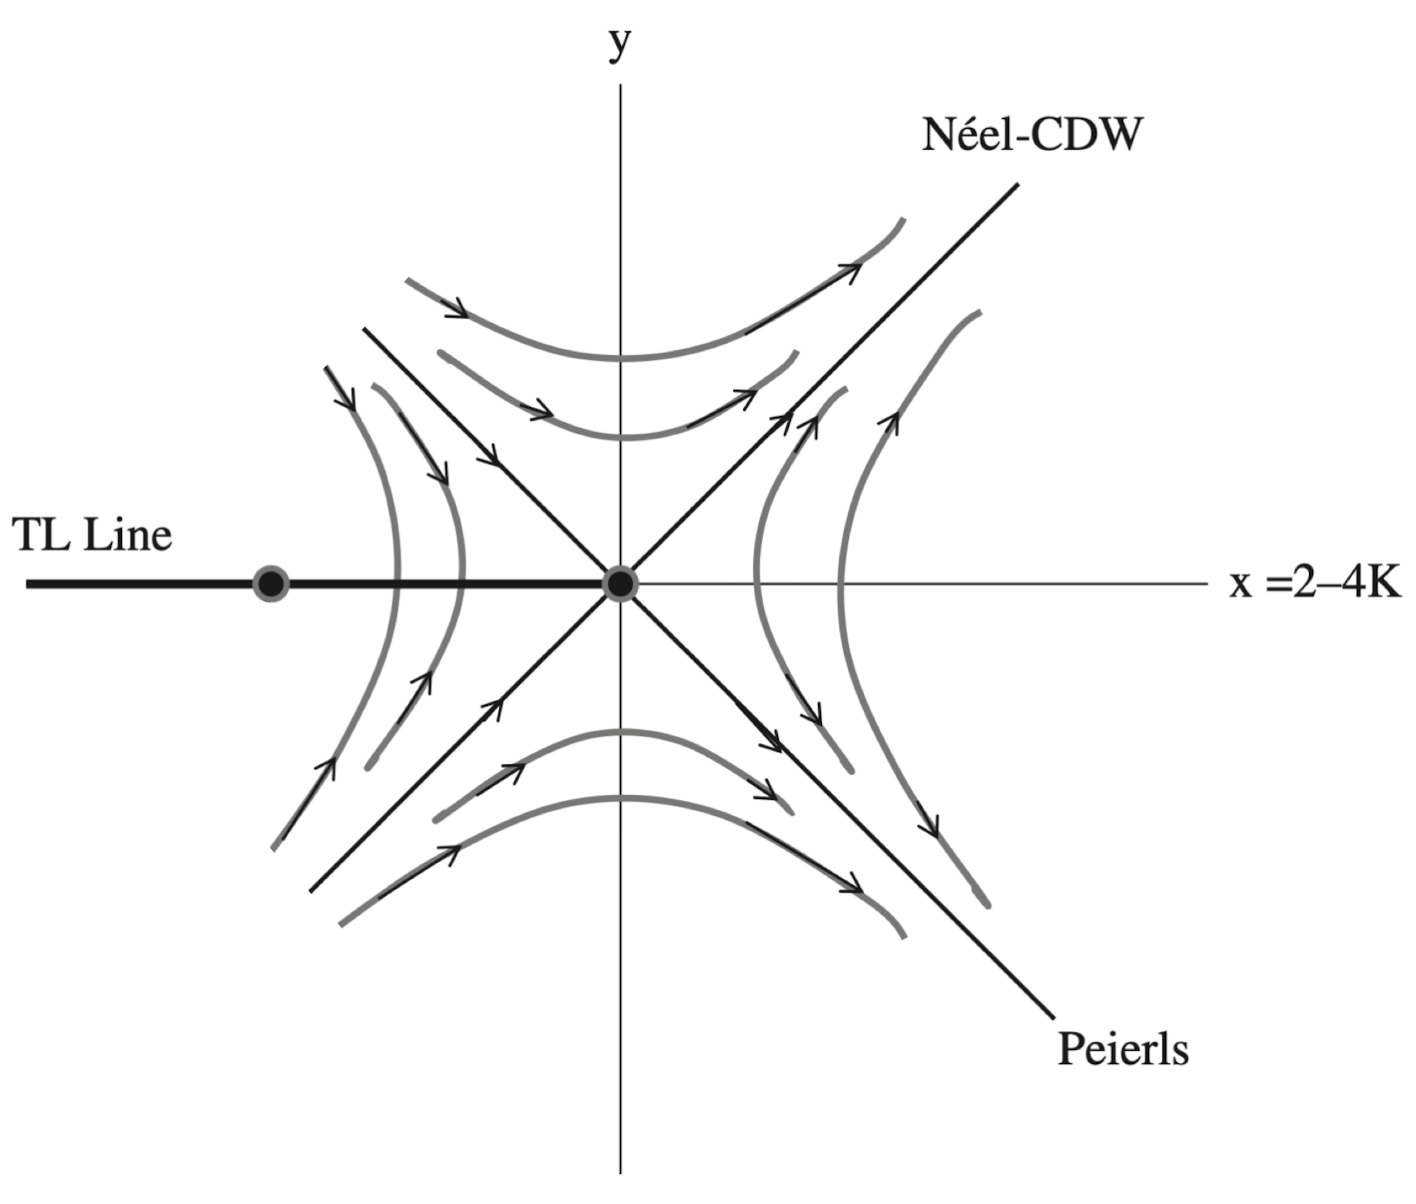
\includegraphics[width=0.5\linewidth]{pics/LL-RG-flow}
	\caption{KT RG-flow.}
	\label{fig:FL-RG-flow}
\end{figure}

We see that there are three regimes of the RG flow: in the weak interacting regime, the field theory flows to the Tomonaga-Luttinger (TL) line; for strong interaction, depending on the sign of $y$, the systems develop two charge-density-wave (CDW) order, namely the Neel-CDW and Peierls-CDW.


\subsection{Phase Diagram}

\subsubsection{Tomonaga-Luttinger Liquid}
When $K<\frac{1}{2}$, the interacting cosine term become irrelevant.
In this case, the system is in a liquid state, called the \textit{Tomonaga-Luttinger liquid}.
The system on the TL line is described by the non-interacting Hamiltonian:
\begin{equation}
	H = \int \frac{dx}{K} \frac{1}{2}\left[K \Pi^2 + \frac{1}{K}(\partial_x\phi)^2 \right],
\end{equation}
As discussed, we can define a new set of variables to map the Hamiltonian to that of the original bosonic model:
\begin{equation}
\begin{aligned}
	\phi' &= \frac{\phi'_-+\phi'_+}{\sqrt 2} = \frac{\phi}{\sqrt{K}} = \frac{\phi_-+\phi_+}{\sqrt{2K}} \\
	\theta' &= \frac{\phi'_--\phi'_+}{\sqrt 2} = \sqrt{K} \theta = \sqrt{\frac{K}{2}}(\phi_--\phi_+).
\end{aligned}
\end{equation}
The fermion mode is
\begin{equation}
\begin{aligned}
	\psi_{\pm}(x) &= \frac{1}{\sqrt{2\pi a}} \exp\left[-i\sqrt{2\pi} \phi'_{\pm}(x) \right] \\
	&= \frac{1}{\sqrt{2\pi a}} \exp\left\{-i\sqrt{2\pi} \left[K_\pm \phi_+(x)+ K_\mp \phi_-(x) \right]\right\},
\end{aligned}
\end{equation}
where 
\begin{equation}
	K_\pm \equiv \frac{K^{\frac{1}{2}} \pm K^{-\frac{1}{2}}}{2}.
\end{equation}
The Greens function is (assume $\tau>0$):
\begin{equation}
	-G_{\pm}(x,\tau) 
	= \frac{1}{2\pi a} e^{2\pi \langle \phi'_\pm(x,\tau)\phi'_\pm(0) - \phi'_\pm(0)\phi'_\pm(0) \rangle}
\end{equation}
The bosonic correlation is
\begin{equation}
\begin{aligned}
	\langle \phi'_\pm(x,\tau)\phi'_\pm(0) \rangle
	&= K_\pm^2 \langle \phi_+(x,\tau)\phi_+(0)\rangle + K_\mp^2 \langle\phi_-(x,\tau)\phi_-(0)\rangle \\
	&= \frac{K_\pm^2}{2\pi}\ln \frac{L/2\pi}{a-ix+\tau} + \frac{K_\mp^2}{2\pi}\ln \frac{L/2\pi}{a+ix +\tau}
\end{aligned}
\end{equation}
So that
\begin{equation}
\begin{aligned}
	-G_{\pm}(x,\tau) 
	&= \frac{1}{2\pi a} \left[\frac{a}{a + \tau - ix}\right]^{K_\pm^2} \left[\frac{a}{a + \tau + i x}\right]^{K_\mp^2} \\
	&= \frac{1}{2\pi} \frac{1}{a + \tau \mp ix} \left[\frac{a^2}{a^2+x^2+\tau^2}\right]^{K_-^2}
\end{aligned}
\end{equation}
Note that when $K=0$, $K_-=0$, and the theory agrees with the free fermion prediction:
\begin{equation}
	-G(x, 0^+) = \frac{1}{2\pi} \frac{1}{a-ix}
	= \int \frac{dk}{2\pi} e^{ikx-ak} \theta(k)
\end{equation}
However, when $K_- \ne 0$, the additional factor will smear the pole to a brach cut. 
To see this, note that from the dimensional analysis, the Green's function is of anomalous dimension $-K_-^2$.
In the momentum space, this means that the Green's function scales as
\begin{equation}
	G(k,\omega) \sim (k,\omega)^{K_-^2}.
\end{equation}
This implies that the density 
\begin{equation}
	n(k) = n_0 + c k^{K_-^2}.
\end{equation}


\subsubsection{Charge Density Wave Order}
We first consider the case where $y>0$ is sufficiently large. 
Consider
\begin{equation}
	\cos\left[\sqrt{16\pi}\phi(x)\right] = \frac{1}{2} - \sin^2\left[\sqrt{4\pi}\phi(x)\right].
\end{equation}
The energy is minimized if 
\begin{equation}
	\sin\left[\sqrt{4\pi}\phi(x)\right] = \pm 1.
\end{equation}
Note that in our bosonization dictionary,
\begin{equation}
	\psi_{\pm}^\dagger(x)\psi_{\mp}(x) = \frac{1}{2\pi a} e^{\pm i\sqrt{4\pi}\phi(x)},
\end{equation}
so that
\begin{equation}
	\frac{i}{\pi a} \sin\left[\sqrt{4\pi}\phi(x)\right] = \psi_{+}^\dagger(x)\psi_{-}(x)-\psi_{-}^\dagger(x)\psi_{+}(x).
\end{equation}
We know for the Neel-CDW phase, the order parameter is
\begin{equation}
	i\left\langle \psi_{+}^\dagger(x)\psi_{-}(x)-\psi_{-}^\dagger(x)\psi_{+}(x) \right\rangle.
\end{equation}

On the other hand, for $y<0$, consider
\begin{equation}
	\cos\left[\sqrt{16\pi}\phi(x)\right] = -\frac{1}{2} + \cos^2\left[\sqrt{4\pi}\phi(x)\right].
\end{equation}
The energy is minimized if 
\begin{equation}
	\cos\left[\sqrt{4\pi}\phi(x)\right] = \pm 1.
\end{equation}




\subsection{One-dimensional Hubbard Model}
Now we consider the fermion with spin.
The Hubbard model has a non-interacting part,
\begin{equation}
	H_{0}=-\frac{1}{2} \sum_{s, n}\left[\psi_{s}^{\dagger}(n) \psi_{s}(n+1)+\text { h.c. }\right]+\mu \sum_{s, n} \psi_{s}^{\dagger}(n) \psi_{s}(n),
\end{equation}
where $s=\uparrow, \downarrow$ are two possible spin orientations. We do not assume $k_F = \frac{\pi}{2}$ at this point, and use a general chemical potential $\mu$.
Following the usual route, we get two copies of the spinless model:
\begin{equation}
	H_{0}=\sum_{s} \int \frac{d k}{2 \pi} (\mu-\cos k) \psi_{s}^{\dagger}(k) \psi_{s}(k),
\end{equation}
and the continuum version:
\begin{equation}
\begin{aligned}
	H_0 &= v_F \sum_{s} \int d x \left[
		\psi_{s+}^{\dagger}(x)\left(-i \partial_{x}\right) \psi_{s+}(x) +
		\psi_{s-}^{\dagger}(x)\left( i \partial_{x}\right) \psi_{s-}(x)
	\right] \\
	&= \frac{v_F}{2} \sum_s \int d x \left[\Pi_{s}^{2}+\left(\partial_x \phi_{s}\right)^{2}\right].
\end{aligned}
\end{equation}
Let us now turn on the Hubbard interaction,
\begin{equation}
	H_{\mathrm{int}}=U \sum_{n} \psi_{\uparrow}^{\dagger}(n) \psi_{\uparrow}(n) \psi_{\downarrow}^{\dagger}(n) \psi_{\downarrow}(n),
\end{equation}
where $\psi_{\uparrow}, \psi_{\downarrow}$ stand for the original non-relativistic fermion. 
The Hubbard interaction is just the extreme short-range version of the screened Coulomb potential between fermions. 
Due to the Pauli principle, only opposite-spin electrons can occupy the same site.

Let us now express this interaction in terms of the Dirac fields:
\begin{equation}
	\psi_{\uparrow}^{\dagger}  \psi_{\uparrow} \psi_{\downarrow}^{\dagger} \psi_{\downarrow} 
	= \left[\psi_{\uparrow+}^{\dagger} \psi_{\uparrow+}+\psi_{\uparrow-}^{\dagger} \psi_{\uparrow-}+
	\left(\psi_{\uparrow+}^{\dagger} \psi_{\uparrow-} e^{-2 i K_{\mathrm{F}} n}+\text{h.c.}\right)\right] 
	\times(\uparrow \rightarrow \downarrow).
\end{equation}
If we expand out the products and keep only the parts with no rapidly oscillating factors, we will, for generic $k_F$, get the following terms:
\begin{equation}
	H_{\mathrm{int}} = U\left(j_{0 \uparrow} j_{0 \downarrow}\right) + U\sum_n \left(\psi_{\uparrow+}^{\dagger}(n) \psi_{\uparrow-}(n) \psi_{\downarrow-}^{\dagger}(n) \psi_{\downarrow+}(n)+\text{h.c.}\right),
\end{equation}
where
\begin{equation}
	U\left(j_{0 \uparrow} j_{0 \downarrow}\right)
	= \sum_n \left(\psi_{\uparrow+}^{\dagger} \psi_{\uparrow+}+\psi_{\uparrow-}^{\dagger} \psi_{\uparrow-}\right)\left(\psi_{\downarrow+}^{\dagger} \psi_{\downarrow+}+\psi_{\downarrow-}^{\dagger} \psi_{\downarrow-}\right)
\end{equation}
If we now bosonize these terms as per the dictionary, we get, in the continuum,
\begin{equation}
	H_{\mathrm{int}} = U\left[\frac{\partial_x \phi_{\uparrow} \partial_x \phi_{\downarrow}}{\pi}+\frac{1}{2\pi^{2} \alpha^{2}} \cos \sqrt{4 \pi}\left(\phi_{\uparrow}-\phi_{\downarrow}\right)\right]
\end{equation}
We can now separate the theory into two parts by introducing charge and spin fields $\phi_{c}$ and $\phi_{s}$:
\begin{equation}
	\phi_{c/s}=\frac{\phi_{\uparrow} \pm \phi_{\downarrow}}{\sqrt{2}}.
\end{equation}
The parametrization bring the first term in the interaction to a free theory:
\begin{equation}
\begin{aligned}
	\partial_x \phi_{\uparrow} \partial_x \phi_{\downarrow}
	&= \frac{1}{2} \partial_x (\phi_{c}+\phi_s) \partial_x (\phi_c-\phi_s) \\
	&= \frac{1}{2} \left[(\partial_x \phi_c)^2 + (\partial_x \phi_s)^2\right].
\end{aligned}
\end{equation}
The Hamiltonian then become decoupled:
\begin{equation}
	H =H_{c}+H_{s},
\end{equation}
where the charge and spin part of the Hamiltonian are:
\begin{equation}
\begin{aligned}
	H_{c} &=\int \frac{dx}{2 K_c}\left[K_{c} \Pi_{c}^{2}+\frac{1}{K_{c}}\left(\partial \phi_{c}\right)^{2}\right], \\
	H_{s} &=\int \frac{dx}{2 K_s} \left[K_{s} \Pi_{s}^{2}+\frac{1}{K_{s}}\left(\partial \phi_{s}\right)^{2}+\frac{U}{2 \pi^{2} \alpha^{2}} \cos \sqrt{8 \pi} \phi_{s}\right],
\end{aligned}
\end{equation}
where 
\begin{equation}
	K_{c / s} =\frac{1}{\sqrt{1 \pm \frac{U}{\pi}}}.
\end{equation}
The fact that $K_{s} \neq K_{c}$ means that charge and spin move at different velocities. 
This \textit{spin-charge separation} cannot be understood in terms of interacting electrons whose charge and spin would be irrevocably bound. 
This is more evidence of the demise of the quasiparticle, adiabatically connected to the primordial fermion.


\chapter{Topological Field Theory}

\section{Chern-Simons Theory}
Assume the action of the microscopical theory has the form $S[\psi_i]$, where $\{\psi_i\}$ denotes all degrees of microscopical freedom.
If the system has the U(1) symmetry, we can always rewrite the field theory as a gauge theory:
\begin{equation}
	S[\psi_i; A] = S[\psi_i] + \int d^dx\ j^\mu(x) A_\mu(x),
\end{equation}
where the current $j^\mu$ is the Noether current.
The gauge field $A^\mu(x)$ is regarded as the back ground field which has no dynamics.
If we are interested in the low-energy physics, especially for gapped system, the ground state physics, we can formally integrate out other degrees of freedom, the resulting effective theory has only the gauge degree of freedom:
\begin{equation}
	Z_{\mathrm{eff}}[A] = \int D[\psi_i] e^{i S[\psi_i;A]}.
\end{equation}
In this section, we consider the effective gauge field on $(2+1)$-dimensional space-time.
The effective action should also be gauge-invariant.
The allowed terms include
\begin{equation*}
	A \wedge dA,\ dA \wedge dA,\ \text{higher order terms}.
\end{equation*}
From dimensional analysis, the first term is most relevant in the low-energy.
Such effective theory is the \textit{Chern-Simons theory}:
\begin{equation}
	S_{\mathrm{CS}} = \frac{k}{4\pi}\int d^3 x\ \varepsilon_{\mu\nu\rho} A^\mu \partial^\nu A^\rho.
\end{equation}


    
\end{document}
